%% CSoNet 2026 Journal Track submission (Journal of Combinatorial Optimization)
%% Build: pdflatex main && bibtex main && pdflatex main && pdflatex main

\documentclass[pdflatex,sn-mathphys-ay]{sn-jnl}

\usepackage{amsmath,amssymb,amsthm}
\usepackage{booktabs}
\usepackage{graphicx}
\usepackage{algorithm}
\usepackage{algpseudocode}

\theoremstyle{thmstyleone}
\newtheorem{theorem}{Theorem}
\newtheorem{proposition}[theorem]{Proposition}
\newtheorem{corollary}[theorem]{Corollary}
\newtheorem{lemma}[theorem]{Lemma}
\newtheorem{fact}{Fact}
\theoremstyle{thmstyletwo}
\newtheorem{assumption}{Assumption}
\newtheorem{remark}{Remark}
\newtheorem{definition}{Definition}
\theoremstyle{thmstylethree}
\newtheorem{example}{Example}

\raggedbottom

\begin{document}

\title[Minimum Weighted Hazard-Exposure Dispatch]{Minimum Weighted
Hazard-Exposure Dispatch: A Scheduling View with Machine-Checked Proofs
and a Wildfire Case Study}

\author*[1]{\fnm{Quang-Vinh} \sur{Dang}}\email{vinh.dq4@buv.edu.vn}
\author[2]{\fnm{Minh Ngoc} \sur{Dinh}}\email{minh.dinh@maeducation.com}
\author[1]{\fnm{Hoang-Viet} \sur{Vu}}\email{30066555@st.buv.edu.vn}
\author[3]{\fnm{Phuc-Son} \sur{Nguyen}}\email{son.np3393@ueh.edu.vn}

\affil*[1]{\orgname{British University Vietnam}, \orgaddress{\city{Hung
Yen}, \country{Vietnam}}}
\affil[2]{\orgname{Millennia Education}, \orgaddress{\city{Ho Chi Minh
City}, \country{Vietnam}}}
\affil[3]{\orgname{UEH University}, \orgaddress{\city{Ho Chi Minh
City}, \country{Vietnam}}}

\abstract{We study a dispatch-scheduling problem arising when a single
depot must send a vehicle or crew to sites before a spreading hazard
(flood, wildfire, contamination plume) reaches them. Each site has a
round-trip dispatch time, a hazard-arrival deadline and a criticality
weight; the objective is a dispatch order maximizing the total weight of
sites served in time. We call this Minimum Weighted Hazard-Exposure
Dispatch (MWHED) and show it is exactly the classical problem
$1\|\sum w_jU_j$, so most of its theory is inherited: weak
NP-hardness, a Lawler--Moore dynamic program, a value-scaling FPTAS, and
a matroid greedy algorithm for equal dispatch times with any number of
vehicles. We present these in a self-contained form for a transportation
audience and mark precisely what is classical. What the dispatch setting
adds is modest and specific: hardness persists when the hazard-arrival
time is the same at every site (with weights proportional to dispatch
times); the depot round-trip model is a conservative bound on a chained
route; and the FPTAS has a guarantee, best possible for the scheme, that
is sharper than the textbook $1-\epsilon$. Natural heuristics have
unbounded worst-case ratio. The algorithms are checked against exhaustive
search and the theory is machine-checked in Lean~4. A case study of the
2018 Camp Fire, built from hazard-arrival times that NIST documents for
each community, shows in this model that the exact optimum inherits the
assumed response speed: planned at a speed above $68$~km/h it is on time
in only $16\%$ of perturbed scenarios, planned at any lower speed it
retains $99.7\%$ of the optimum.}

\keywords{scheduling under deadlines, computational complexity,
approximation algorithms, matroids, disaster response, formal
verification}

\maketitle

% ══════════════════════════════════════════════════════════════════
\section{Introduction}\label{sec:intro}

A recurring operational problem in infrastructure and emergency-response
networks is deciding, from a single depot, in what order to dispatch a
vehicle or crew to a set of sites that are each racing against a
spreading hazard. A wildfire crew choosing which structures to defend
before the fire front arrives, a utility company dispatching repair
trucks to substations before a cascading outage propagates to them, and
a flood-response team evacuating or servicing neighborhoods before
rising water reaches them all face the same underlying decision: given
a known rate at which a hazard is spreading, and a known cost of
reaching each site from a common depot, in what order should sites be
visited to save as much value as possible before the hazard reaches
each one in turn?

This decision is a scheduling problem, not merely a routing one. Once
every visit is a self-contained round trip from a single depot---the
standard topology for a technician, repair-crew, or single-vehicle
emergency-response dispatch base---the cost of visiting a site does not
depend on which site was visited immediately before it, only on the
cumulative time already spent. The question is then purely one of
\emph{order}: which sites to reach early, which to defer, and which to
concede to the hazard, given that each site $i$ becomes ``exposed''
once the cumulative dispatch time exceeds its known hazard-arrival
deadline $d_i$, at a loss of $w_i$.

The three motivating settings above share a further feature that makes
the \emph{ordering} decision, rather than the underlying routing or
hazard-forecasting problem, the right object of study. In each case,
the hazard's own spread is typically produced by a separate, already
well-developed forecasting step---a wildfire-spread simulator driven by
fuel load, wind, and terrain; a cascading-failure model for a power
network; a hydrological model for a flood plain---so that, by the time
a dispatcher is choosing a visiting order, each site's arrival deadline
$d_i$ is already a given input, not something to be modeled jointly
with the dispatch decision. Similarly, the round-trip dispatch time
$p_i$ is typically fixed by the depot's location and the local road or
access network, and is known before dispatch begins. What remains
undetermined, and squarely a combinatorial decision, is the
\emph{order} in which a single crew or vehicle should visit sites once
$p_i$ and $d_i$ are fixed---exactly the question MWHED isolates. This
separation of concerns (forecast the hazard and fix the travel network
first; optimize the dispatch order second) mirrors how the wildfire
operations-research literature we discuss in Section~\ref{sec:related}
is typically organized, and is what lets us give a precise
complexity and algorithmic picture of the ordering question alone,
rather than a heuristic for the joint problem.

We formalize this as Minimum Weighted Hazard-Exposure Dispatch
(MWHED). It is worth saying at the outset, and Section~\ref{sec:model}
proves it, that MWHED is \emph{exactly} the classical single-machine
problem $1\|\sum w_jU_j$ of maximizing the weighted number of on-time
jobs. Most of its theory is therefore inherited from scheduling theory,
and we do not claim a new algorithmic technique. The paper is a
self-contained and carefully verified treatment of this problem in
transportation vocabulary, with a small number of additions that depend
on the dispatch setting. We separate the two kinds of content.

\emph{Classical results, restated with complete proofs} (marked
``classical'' in Table~\ref{tab:summary}):
\begin{enumerate}
\item MWHED is weakly NP-hard, by a direct reduction from
\textsc{Partition} that uses only the equal-deadline case, which is the
0/1 knapsack problem (Theorem~\ref{thm:hardness}); the hardness of job
sequencing with penalties is already in \citet{karp1972}.
\item An exact pseudo-polynomial dynamic program derived from an
earliest-deadline-first exchange argument (Theorem~\ref{thm:dp}); this is
the Lawler--Moore program \citep{lawlermoore1969}.
\item A value-scaling FPTAS (Theorem~\ref{thm:fptas}); approximation
schemes for this problem are classical \citep{sahni1976,gensl1981}.
\item A matroid greedy algorithm for equal dispatch times and any number
of vehicles, identical or with different dispatch times
(Theorem~\ref{thm:equalp}). This is the scheduling of unit-time jobs on
identical or uniform machines, for which $O(n\log n)$ algorithms are
known \citep{lawler1976,dessouky1990}; we include a self-contained proof.
\item A classification of the restrictions in which some of the dispatch
times, weights and deadlines are constant
(Theorem~\ref{thm:classification}); it is an elementary corollary of
items~1 and~4 and of Moore's algorithm.
\end{enumerate}
\emph{What the dispatch setting adds.} These additions are modest, and
we state them as such:
\begin{enumerate}
\setcounter{enumi}{5}
\item \emph{A refined FPTAS analysis.} The textbook guarantee
$1-\epsilon$ is not attained: the scheme of Theorem~\ref{thm:fptas}
guarantees $\rho_{n,\epsilon}>1/(1+\epsilon)$, and this constant is
best possible for the scheme as stated, without the optional completion
step (Proposition~\ref{prop:tight}); rescaling $\epsilon$ recovers the
classical bound, so the gain is a constant, not an order.
\item \emph{The two readings of a deadline.} Under the arrival reading
(the crew must arrive before the hazard does), MWHED stays weakly
NP-hard even when the hazard-arrival time is the same at every site and
weights are proportional to dispatch times
(Proposition~\ref{prop:consth}; to our knowledge not stated before); and the depot round-trip model is a
conservative bound on a route that chains the sites
(Proposition~\ref{prop:spoke}), which says when the round-trip premise is
appropriate and when it is not (when travel times form a metric).
\item \emph{Worst-case examples.} Dispatching in deadline order, with or
without skipping, and a weighted greedy repair all have unbounded
worst-case ratio (Propositions~\ref{prop:naive} and~\ref{prop:repair});
the examples are elementary, and on random instances the greedy repair is
within $1\%$ of the optimum on average.
\item \emph{Verification.} Every algorithm is checked against exhaustive
search (Section~\ref{sec:verify}), and the statements and proofs of the
lemmas, theorems and propositions above, except complexity-class and
running-time claims, are machine-checked in Lean~4 (see the Data
Availability statement for the precise scope; the algorithms'
implementations are checked by testing, not by Lean).
\item \emph{A case study on documented data.} A Camp Fire instance built
from the hazard-arrival times that NIST documents for each community,
compared with a chained-route model, with a sensitivity analysis and a
sample-average plan (Section~\ref{sec:campfire}).
\end{enumerate}
To keep the argument concrete, Sections~\ref{sec:model}
and~\ref{sec:theory} carry a single four-site running example through the
results, worked out by hand alongside each proof.

The remainder of this paper is organized as follows.
Section~\ref{sec:related} positions MWHED against the scheduling,
deadline-routing and disaster-response literatures and states precisely
what is classical. Section~\ref{sec:model} defines MWHED and
establishes the earliest-deadline-first lemma every later result
depends on. Section~\ref{sec:theory} proves the results above.
Section~\ref{sec:experiments} reports the numerical study and the case
study. Section~\ref{sec:discussion} discusses extensions (several
vehicles, a moving depot, and uncertain parameters) and precisely what
each breaks in our analysis, and Section~\ref{sec:conclusion}
concludes. Two appendices give an exhaustive hand-verification of the
running example and a spelled-out derivation of the FPTAS bound.

% ══════════════════════════════════════════════════════════════════
\section{Related work}\label{sec:related}

\textbf{Scheduling with deadlines.} MWHED, once its transportation
framing is stripped away, is the classical single-machine problem of
maximizing the weighted number of on-time jobs, equivalently minimizing
the weighted number of late jobs, $1\|\sum w_jU_j$ in the standard
three-field notation (job $j$ has processing time $p_j$, due date $d_j$
and weight $w_j$; $U_j=1$ if it is late). It is also a single-machine
scheduling-with-rejection (order acceptance) problem \citep{shabtay2013}.
\citet{moore1968} gives an $O(n\log n)$ algorithm for the
\emph{unweighted} case: process jobs in earliest-due-date order, and
whenever the running schedule becomes infeasible, permanently discard the
scheduled job with the largest processing time (the Moore--Hodgson
algorithm). \citet{lawler1976} notes that the rule extends to oppositely
ordered (agreeable) processing times and weights,
$p_i<p_j\Rightarrow w_i\ge w_j$, a class that contains both the
equal-weight and the equal-processing-time cases. For the general
weighted case, \citet{lawlermoore1969} give a dynamic program over jobs
in due-date order and total processing time that runs in $O(nP)$ time,
$P=\sum_jp_j$; this is our Theorem~\ref{thm:dp}. The problem is weakly
NP-hard: job sequencing with deadlines and penalties is among Karp's
original problems \citep{karp1972}, and an instance with a common due
date is a 0/1 knapsack instance \citep{gareyjohnson1979}; complexity
surveys include \citet{lenstra1977}. Approximation schemes are classical
too: \citet{sahni1976} gives rounding-based approximation algorithms for
single-processor job sequencing with deadlines, which is the same
problem, and \citet{gensl1981} give a faster scheme; both build on the
knapsack schemes of \citet{ibarrakim1975}, \citet{lawler1979} and
\citet{kellerer1999,kellerer2004}.

Hence our Theorems~\ref{thm:hardness} and~\ref{thm:dp}, and the scheme of
Theorem~\ref{thm:fptas}, are re-derivations in our notation, not new
techniques. The same is true of
Theorem~\ref{thm:equalp}: for equal processing times (unit jobs) the
weighted number of late jobs is polynomial on one machine, on identical
machines and on uniform machines, with $O(n\log n)$ algorithms due to
\citet{lawler1976} and \citet{dessouky1990}; see the surveys
\citet{baptiste2004} and \citet{kravchenkowerner2011}, and
\citet{bruckerkravchenko2006} for equal-processing-time jobs and the
weighted number of late jobs. With release dates the single-machine
problem with equal processing times is still polynomial
\citep{baptiste1999}, whereas the \emph{unweighted} problem on $m$
identical machines with equal processing times and release dates is
NP-hard and $W[2]$-hard parameterized by $m$ \citep{heegermolter2025}. The
classification of Theorem~\ref{thm:classification} is an elementary
corollary of these facts, and the more natural tractable boundary in the
literature is Lawler's agreeable-weights case rather than constancy.

This classical problem remains an active research topic.
\citet{hejl2022} give a refined pseudo-polynomial dynamic program for the
practically important ``strongly correlated'' regime (where processing
times and weights are close in value), and \citet{hermelin2024} improve
the Lawler--Moore-style program's running time via
$(\max,+)$-convolution techniques, an algorithmic refinement orthogonal
to Theorem~\ref{thm:dp} and compatible with it. For the special case
$w_j=p_j$, which is the case our hardness reduction uses (minimizing the
total processing time of late jobs), there is a fine-grained line of work
with near-linear pseudo-polynomial algorithms
\citep{bringmann2022,klein2023,fischer2025theoretics}.
\citet{heegerhermelin2024} prove that $1\|\sum w_jU_j$ is $W[1]$-hard
parameterized by the number of distinct processing times and also by the
number of distinct weights; so, unless $\mathrm{FPT}=W[1]$, there is no
$f(k)\cdot\mathrm{poly}(n)$ algorithm in the number $k$ of distinct
dispatch times (or criticality levels), and a small number of distinct
values does not make the problem easy in the fixed-parameter sense. We
make no claim about two or more distinct values beyond this; the case
$k=1$ is the tractable case of Theorem~\ref{thm:equalp} (or
Moore--Hodgson, for equal weights). On the heuristic side,
\citet{antonov2026} give a data-driven (machine-learning-guided) heuristic
for the same objective, a more sophisticated relative of the weighted
greedy-repair heuristic we use as an empirical baseline in
Section~\ref{sec:experiments}.

\textbf{Real-time systems.} Earliest-deadline-first ordering is also
central to real-time scheduling \citep{liulayland1973}, where the question
is whether \emph{every} task meets its deadline; MWHED presupposes that
some sites will be lost, which is the optimization question behind
Theorem~\ref{thm:hardness}.

\textbf{Approximation.} The 0/1 knapsack problem admits a fully
polynomial-time approximation scheme via scaling and rounding of item
values, due to \citet{ibarrakim1975}, with later improvements
\citep{lawler1979,kellerer1999,kellerer2004,jin2019,chen2025fptas}; the
same technique applies to job sequencing with deadlines
\citep{sahni1976,gensl1981}, and Theorem~\ref{thm:fptas} is this
construction written for MWHED. The one point at which the presentation
differs from knapsack is that there is no single shared capacity (each
site has its own deadline), so the value-indexed table must test
feasibility against each site's $d_i$; this is easy in deadline order
(Lemma~\ref{lem:g}). A general framework for when a dynamic program
yields an FPTAS is due to \citet{woeginger2000}. Our contribution here is
only the sharper analysis of Theorem~\ref{thm:fptas}, with the exactly
tight constant of Proposition~\ref{prop:tight}. For several vehicles
with a common deadline MWHED contains the multiple knapsack problem,
which has a PTAS \citep{chekuri2005}; whether the value-scaling scheme
extends to a fixed number of vehicles is open here.

\textbf{Matroids and greedy algorithms.} The equal-processing-time case
of Theorem~\ref{thm:equalp} is an instance of the classical problem of
scheduling unit-time jobs with deadlines to maximize total profit, whose
feasible job sets form a (transversal) matroid on which the greedy
algorithm is optimal \citep{edmonds1971}; we follow the treatment in
\citet{kortevygen2018}. This matroid structure is exactly what breaks
once dispatch costs become heterogeneous, which is why
Theorem~\ref{thm:equalp}'s greedy algorithm has no counterpart for
general MWHED. Concretely, in the equal-deadline restriction (which
Theorem~\ref{thm:hardness} identifies with 0/1 knapsack of capacity
$D$), take three sites with dispatch times $2,1,5$ and a common
deadline $D=5$: $\{3\}$ (the size-$5$ site alone) is feasible and
already uses the entire capacity, while $\{1,2\}$ (total size $3$) is
also feasible; but neither remaining site can be added to $\{3\}$ ($5+2$
and $5+1$ both exceed $D=5$), so a feasible set of size $1$ fails to
extend toward a feasible set of size $2$ by any element of the latter,
which is precisely the matroid exchange property failing. This is why a
single large, low-value commitment can block a strictly better pair of
smaller commitments, and is the structural reason
Theorem~\ref{thm:hardness}'s hardness survives even though the matroid
case (Theorem~\ref{thm:equalp}) is easy.

\textbf{Deadline routing.} MWHED sits at the ``no-routing'' end of the
family of selective routing problems with deadlines: orienteering with
time windows \citep{vansteenwegen2011}, the deadline-TSP and its
approximation algorithms \citep{tsitsiklis1992,bansal2004}, and the
traveling salesman problem with profits \citep{feillet2005}. In those
problems the travel time between consecutive sites depends on the
sequence; in MWHED every visit is a round trip from the depot, so the
occupancy of a site is order-independent and the problem is a scheduling
problem with exact algorithms and guarantees. The price is a modelling
premise, which Proposition~\ref{prop:spoke} shows to be conservative when
travel times form a metric: a route that chains the sites can only protect
more.

\textbf{Dispatch under a spreading hazard.} Wildfire suppression is the
application area where the ``race a spreading hazard'' structure has been
studied most directly in the operations research literature, and it
illustrates the point at which our abstraction departs from that
literature's usual level of detail. \citet{rachaniotis2006} schedule a
single fire-fighting resource over several fires using the concept of
deteriorating jobs, the model closest in spirit to ours.
\citet{harris2023} model fire spread via a minimum-travel-time
principle---the fire's arrival time at any point is governed by the
fastest path a flame front can take through spatially varying
fuel and terrain, akin to a shortest-path computation over a
continuous landscape---and decompose the resulting joint
suppression-and-routing decision via logic-based Benders decomposition,
trading exact fire-spread geometry against tractable large-scale
optimization. \citet{avci2024} extend this style of problem to multiple
heterogeneous resource types (e.g., ground crews and aircraft with
different suppression capabilities and travel speeds).
\citet{alvelos2025} go further, jointly optimizing dispatching, the
positioning of resources in anticipation of the fire's advance, and
their routing, in a single integrated model. More recently,
\citet{granda2025} give a mathematical programming formulation for
wildfire suppression resource allocation, and, closest in spirit to our
own complexity results, \citet{delazeri2026} prove NP-completeness for a
landscape-graph model of wildfire suppression resource allocation,
alongside a competitive mixed-integer program and a physics-grounded
(Rothermel fire-spread model) instance generator, an independent hardness
result in essentially our application domain though for a differently
structured (graph-based, simultaneous multi-resource) model. Two recent
systematic reviews position the broader literature: \citet{tezcan2025}
survey optimization approaches to forest-fire suppression, and
\citet{rostamian2026} review 177 papers on wildfire management
optimization under uncertainty and complexity. Across all of these, the
fire's own spatial spread is modeled in detail and coupled tightly to the
routing and positioning decisions; MWHED instead abstracts the hazard's
spread into a per-site deadline, a reduction that is natural once a
simulator has produced arrival-time estimates for each site. The
abstraction is not innocent when the dispatch itself changes the hazard
(as suppression does); the cited joint models exist because of that
coupling, and MWHED applies when the deadlines can be taken as given.

\textbf{Positioning.} MWHED inherits its complexity classification and
its algorithms from scheduling theory
(\citealp{moore1968,lawlermoore1969,lawler1976,dessouky1990,karp1972,sahni1976,gensl1981,hejl2022,hermelin2024,heegerhermelin2024}),
its approximation toolkit from knapsack approximation
(\citealp{ibarrakim1975,lawler1979,kellerer1999,jin2019,chen2025fptas}),
and its motivation from disaster-response operations research
(\citealp{rachaniotis2006,harris2023,avci2024,alvelos2025,granda2025,delazeri2026,tezcan2025,rostamian2026}).
Its theoretical results are, with the exceptions listed in the
introduction, classical ones restated in transportation language;
Table~\ref{tab:summary} in Section~\ref{sec:theory} marks which, and the
paper's claim to value rests on the careful, machine-checked treatment, the
sharper FPTAS analysis, the analysis of the two deadline readings and of
the round-trip premise, and the case study on documented data.

% ══════════════════════════════════════════════════════════════════
\section{Model}\label{sec:model}

\begin{definition}[Minimum Weighted Hazard-Exposure Dispatch]\label{def:mwhed}
An instance of MWHED consists of $n$ sites $1,\dots,n$ and a depot. Each
site $i$ has a round-trip dispatch time $p_i \in \mathbb Z_{>0}$ (the
time to travel from the depot to site $i$ and back, or more generally
the time the depot's single vehicle or crew is occupied while serving
site $i$), a hazard-arrival deadline $d_i \in \mathbb Z_{>0}$ (the known
time at which a spreading hazard reaches site $i$), and a criticality
weight $w_i \in \mathbb Z_{>0}$. A \emph{dispatch order} is a
permutation $\sigma$ of $\{1,\dots,n\}$; the \emph{completion time} of
site $\sigma(k)$ is $C_{\sigma(k)}(\sigma) := \sum_{j=1}^k
p_{\sigma(j)}$, and site $i$ is \emph{on time} under $\sigma$ if $C_i(\sigma)
\le d_i$, otherwise \emph{exposed}. The objective is to choose $\sigma$
maximizing the total on-time weight
\begin{equation}\label{eq:objective}
W(\sigma) := \sum_{i=1}^n w_i \cdot \mathbb 1\bigl[C_i(\sigma) \le
d_i\bigr].
\end{equation}
\end{definition}

Table~\ref{tab:notation} collects the notation introduced in this
definition and used throughout the rest of the paper, for reference.

\begin{table}[h]
\caption{Notation used throughout the paper.}\label{tab:notation}
\begin{tabular}{@{}ll@{}}
\toprule
Symbol & Meaning \\
\midrule
$n$ & number of sites \\
$p_i$ & round-trip dispatch time for site $i$ \\
$d_i$ & hazard-arrival deadline for site $i$ \\
$w_i$ & criticality weight for site $i$ \\
$\sigma$ & a dispatch order (permutation of sites) \\
$C_i(\sigma)$ & completion time of site $i$ under order $\sigma$ \\
$W(\sigma)$ & total on-time weight of order $\sigma$, Eq.~\eqref{eq:objective} \\
$W^\ast$ & the optimal (maximum) value of $W(\sigma)$ \\
$S$ & a subset of sites dispatched on time \\
$P$ & $\sum_{i=1}^n p_i$, the total dispatch time (Theorem~\ref{thm:dp}) \\
$f(i,t)$ & exact DP table: max weight using sites $1..i$, time exactly $t$ \\
$\epsilon$ & FPTAS accuracy parameter, $\epsilon\in(0,1)$ (Theorem~\ref{thm:fptas}) \\
$K$ & FPTAS weight-scaling factor \\
$w_i'$ & scaled weight, $\lfloor w_i/K\rfloor$ \\
$g(i,v)$ & FPTAS's value-indexed dual DP table \\
$D_i$ & latest feasible slot index, equal-size case, $\min\{n,C(d_i)\}$ (Theorem~\ref{thm:equalp}) \\
$m$ & number of vehicles (MWHED-$m$, Section~\ref{sec:equalp}) \\
$\rho_{n,\epsilon}$ & FPTAS guarantee constant (Theorem~\ref{thm:fptas}) \\
\bottomrule
\end{tabular}
\end{table}

Because every visit returns to the depot before the next dispatch
begins, $p_i$ does not depend on which site precedes or follows site
$i$ in the order, the defining structural feature that distinguishes
MWHED from a routing problem and places it in the scheduling family.
This is a modelling premise, not a fact about networks. It is natural for
a hub-and-spoke network and for crews that must return to the depot
(to re-supply, to hand over, or to be debriefed), and, as
Proposition~\ref{prop:spoke} below shows, it is \emph{conservative}
otherwise: a crew that may travel directly between sites can only protect
more.
Minimizing total \emph{exposure cost} $\sum_i w_i(1 - \mathbb
1[C_i(\sigma)\le d_i])$ is equivalent to maximizing $W(\sigma)$, since
$\sum_i w_i$ is a constant of the instance; we work with the
maximization form throughout.

\begin{assumption}[Individually feasible sites]\label{as:feasible}
Every site satisfies $p_i \le d_i$.
\end{assumption}

This is without loss of generality: a site with $p_i > d_i$ cannot be
on time under any dispatch order, even served first, so it can be
deleted from the instance in a preprocessing pass without changing the
optimal value achievable on the remaining sites. One immediate
consequence we use later: the single highest-weight site, dispatched
alone, is itself a feasible subset, so $W^\ast \ge w_{\max} := \max_i
w_i$.

\begin{remark}[Return and arrival readings of the deadline]\label{rem:reading}
Definition~\ref{def:mwhed} counts a site as on time when the vehicle's
\emph{completion} of the whole $p_i$-long occupancy---the round trip,
including the return---happens by $d_i$ (the \emph{return reading}).
When what matters is that the vehicle \emph{arrive} at the site before
the hazard does, only the outbound part $a_i\le p_i$ of the occupancy
must fit: site $i$ is protected iff $C_i-p_i+a_i\le d_i^{\mathrm{haz}}$,
where $d_i^{\mathrm{haz}}$ is the hazard-arrival time. This is the same
test with deadline $d_i:=d_i^{\mathrm{haz}}+(p_i-a_i)$, which for a
symmetric trip is $d_i^{\mathrm{haz}}+p_i/2$. Hence the \emph{arrival
reading} is an instance of Definition~\ref{def:mwhed} with shifted
deadlines, and every \emph{algorithmic} result below applies to it
unchanged; only the input $d_i$ differs. What changes is the meaning of
homogeneity: a constant deadline $d_i$ now corresponds to a hazard-arrival
time $d_i^{\mathrm{haz}}=d_i-p_i/2$ that varies with the dispatch time, so
Theorem~\ref{thm:classification} does not by itself say anything about a
constant hazard-arrival time; Proposition~\ref{prop:consth} proves that
hardness survives that restriction. The two readings can give different answers on the
same data, so a practitioner must state which one the hazard-arrival
times refer to; Section~\ref{sec:campfire} uses the arrival reading.
\end{remark}

\begin{proposition}[The depot round-trip model is conservative]\label{prop:spoke}
Let the depot $0$ and the sites lie in a metric space with symmetric
distance $\delta$, let the crew travel at speed $s$, and put
$a_i:=\delta(0,i)/s$ and $p_i:=2a_i$. Under the arrival reading, site $i$
is protected iff the crew arrives at $i$ by its hazard-arrival time
$h_i$. Fix an order $(i_1,\dots,i_k)$. In the depot round-trip model the
crew arrives at $i_j$ at time $A_j:=\sum_{l<j}p_{i_l}+a_{i_j}$; if it
travels directly from each site to the next it arrives at time
$B_j\le A_j$. Hence every site that the round-trip model protects with an
order is also protected by the chained route with the same order, and the
optimal protected weight of the chained-route problem is at least the
optimum $W^\ast$ of the MWHED instance with $d_i=h_i+p_i/2$.
\end{proposition}

\begin{proof}
$B_j=a_{i_1}+\sum_{l=1}^{j-1}\delta(i_l,i_{l+1})/s$, and
$\delta(i_l,i_{l+1})\le\delta(i_l,0)+\delta(0,i_{l+1})$ by the triangle
inequality, so
$B_j\le a_{i_1}+\sum_{l=1}^{j-1}(a_{i_l}+a_{i_{l+1}})
=2\sum_{l<j}a_{i_l}+a_{i_j}=A_j$.
\end{proof}

The inequality is an equality when the sites lie on different branches of
a star network centred at the depot, and can be strict by a wide margin
when sites are clustered, as in the case study of
Section~\ref{sec:campfire}. The proposition says that, when travel times form a metric (in particular
when the direct roads between sites are open), a depot-spoke optimum is a
\emph{lower bound} on what a crew can protect, which is the safe direction
for planning, and it says when the round-trip premise is
costly: when the sites are close to each other relative to their distance
from the depot.

The following lemma is the structural fact both the dynamic program of
Section~\ref{sec:theory} and the tractability results depend on. It is
the transportation-scheduling analogue of the classical fact that
earliest-due-date order minimizes maximum lateness on a single machine.

\begin{lemma}[Earliest-deadline-first feasibility]\label{lem:edd}
Fix a subset $S \subseteq \{1,\dots,n\}$. There exists a dispatch order
under which every site in $S$ is on time if and only if, when the sites
of $S$ are dispatched first (before any site outside $S$) in order of
non-decreasing deadline $d_i$ (ties broken arbitrarily), every site in $S$
is on time.
\end{lemma}

\begin{proof}
Sufficiency is immediate: the stated order is one such dispatch order.
Conversely, let $S$ be on time under some order $\sigma$ and let $\tau$
be any order that serves the sites of $S$ first, by non-decreasing
deadline. Fix $i\in S$ and let $J$ be the set of sites of $S$ that $\tau$
serves up to and including $i$; then $d_j\le d_i$ for all $j\in J$, and
the completion time of $i$ under $\tau$ is $C_i(\tau)=\sum_{j\in J}p_j$.
Under $\sigma$ the vehicle serves all of $J$ before the last of them,
say $j^\ast$, completes, so $C_{j^\ast}(\sigma)\ge\sum_{j\in J}p_j$.
Hence
\[
C_i(\tau)\ \le\ C_{j^\ast}(\sigma)\ \le\ d_{j^\ast}\ \le\ d_i,
\]
because $\sigma$ is on time for $S$ and $j^\ast\in J$. So $i$ is on time
under $\tau$; as $i$ was arbitrary, the claim follows.
\end{proof}

Lemma~\ref{lem:edd} lets us restrict attention, without loss of
generality, to dispatch orders that serve some subset $S$ first, in
increasing-deadline order, followed by the remaining (necessarily
exposed) sites in any order; the optimization problem becomes that of
choosing $S$ to maximize $\sum_{i\in S} w_i$ subject to the feasibility
condition of Lemma~\ref{lem:edd}.

\begin{example}[A running illustration]\label{ex:running}
Throughout this section we illustrate each result on a single small
instance: four sites with round-trip dispatch times $p=(2,3,1,4)$,
hazard deadlines $d=(4,6,2,9)$, and criticality weights $w=(5,8,3,10)$,
all satisfying Assumption~\ref{as:feasible}. Sorting by increasing
deadline gives the order $3,1,2,4$ (deadlines $2,4,6,9$);
Lemma~\ref{lem:edd} says we may restrict to dispatch orders that serve
some subset $S$ first, in exactly this relative order.

Dispatching every site in this order---the naive policy of simply
visiting sites earliest-deadline-first, with no further
optimization---gives completion times $1,3,6,10$ for sites $3,1,2,4$
respectively; the first three are on time, but site $4$, with deadline
$9$, arrives at cumulative time $10$ and is exposed, losing its full
weight $w_4=10$. This naive order captures only $w_3+w_1+w_2 =
3+5+8=16$ of the total weight $26$.

The optimal choice of $S$ is instead $\{1,2,4\}$, excluding site $3$:
dispatched in deadline order $1,2,4$, completion times are $2,5,9$,
each on time, for a total on-time weight of $W^\ast = 5+8+10=23$---
strictly better than the naive $16$, by deliberately sacrificing site
$3$ (deadline $2$, weight only $3$) to make room for the far more
valuable site $4$. No dispatch order can do better, as
Example~\ref{ex:dp}'s dynamic program table confirms exhaustively. This
gap between naive earliest-deadline dispatch and the true optimum is
what Section~\ref{sec:experiments} measures on random instances.
\end{example}

\begin{figure}[h]
\centering
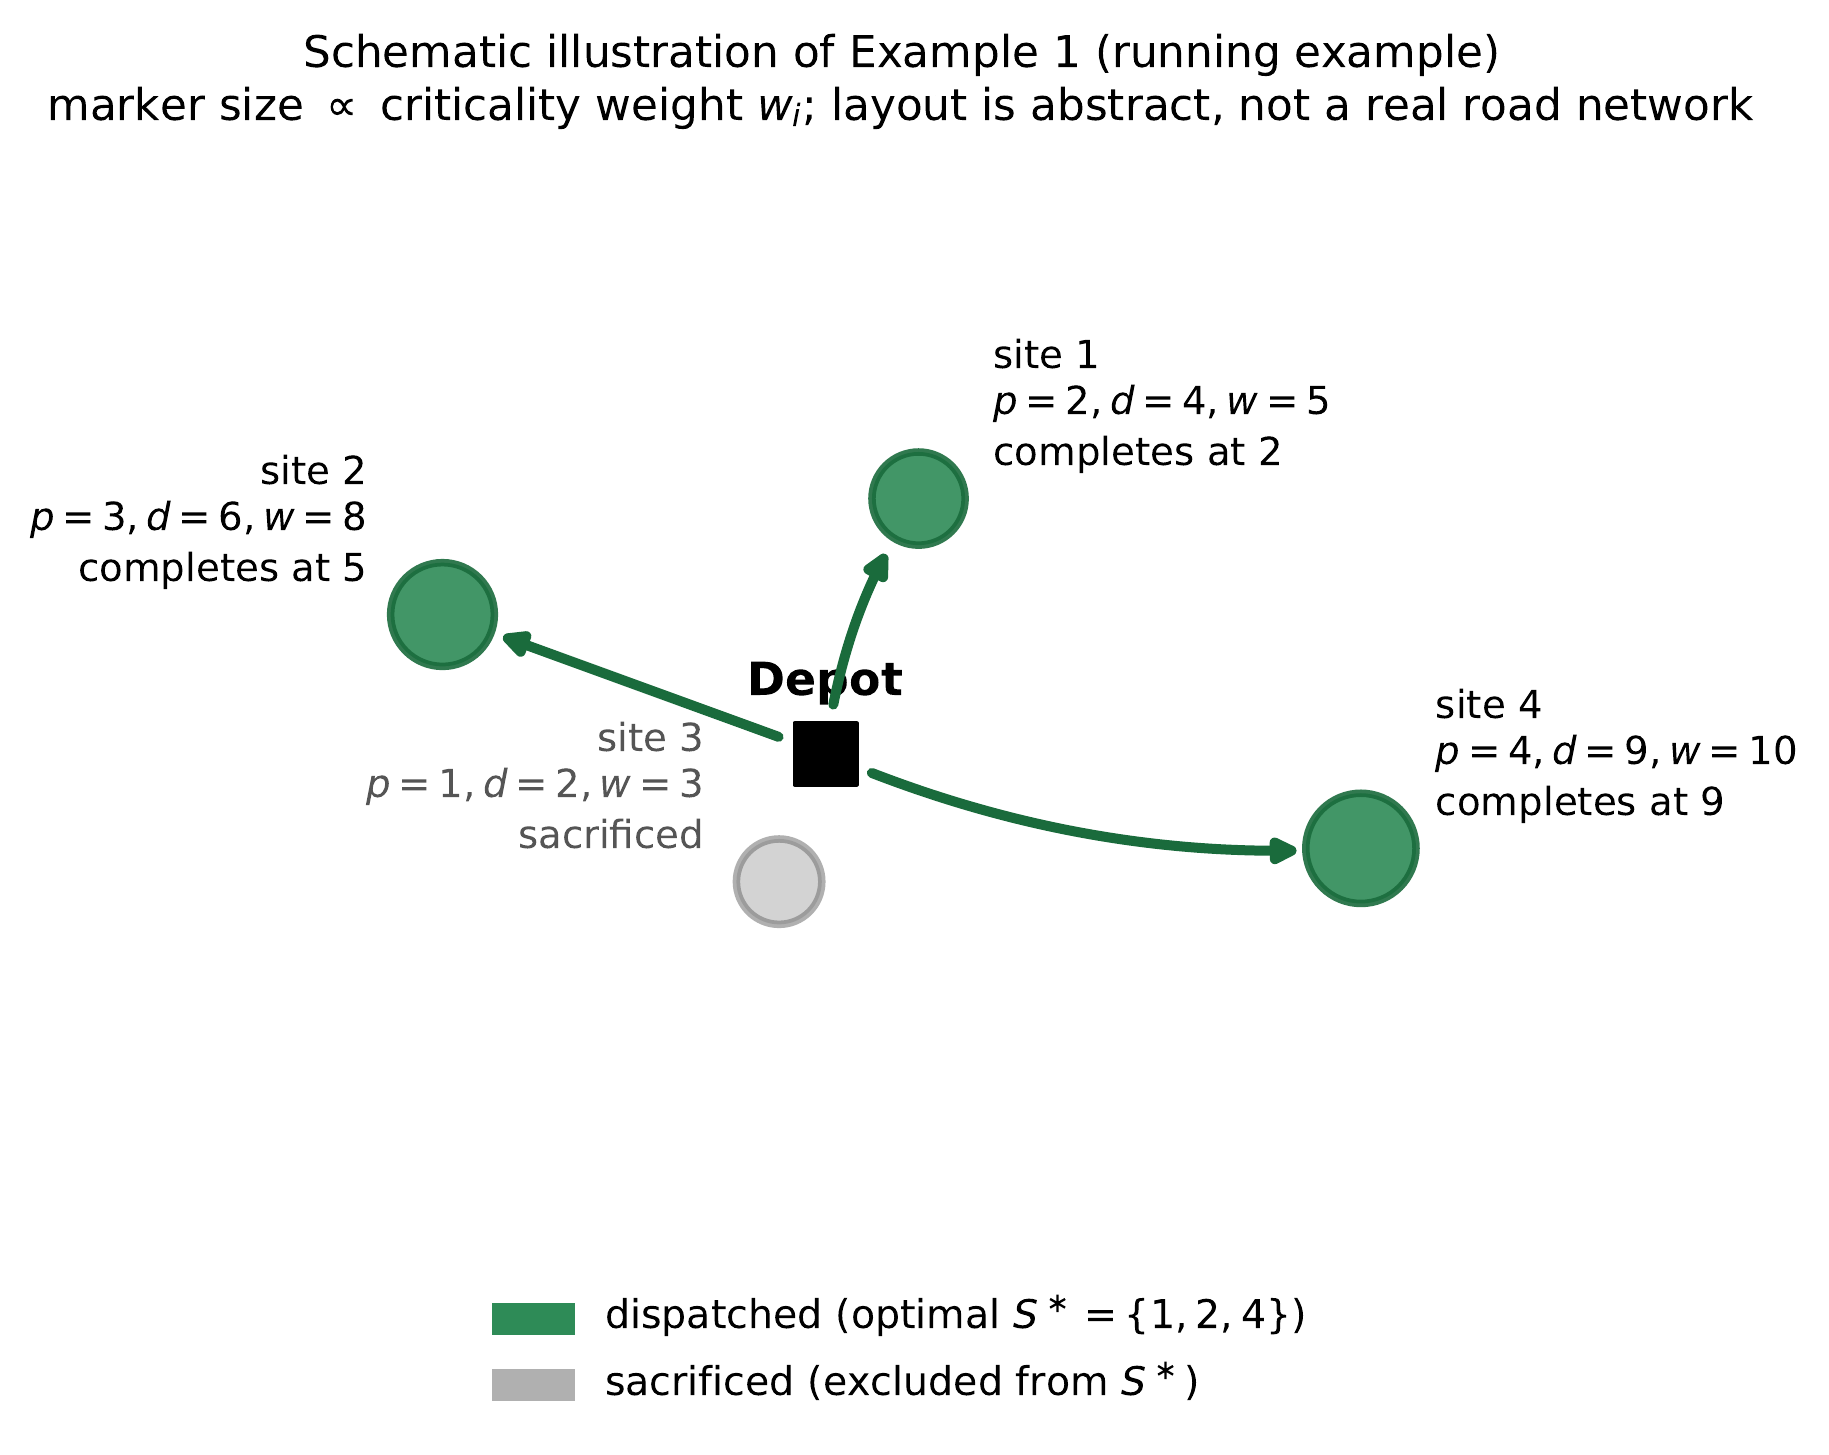
\includegraphics[width=0.75\textwidth]{running_example_schematic.png}
\caption{A schematic illustration of Example~\ref{ex:running}. Site
positions are laid out at a radius proportional to each site's
round-trip dispatch time $p_i$, purely for visual spacing---this is an
abstract schematic of the instance, not a real road network or a
geographic map (MWHED's theory is instance-agnostic and this paper
uses no real-world coordinate data). Marker size is proportional to
criticality weight $w_i$; green markers and arrows show the optimal
dispatch $S^\ast=\{1,2,4\}$ and each site's completion time; the gray
marker is site $3$, sacrificed to make room for the higher-value site
$4$.}\label{fig:running-example}
\end{figure}

% ══════════════════════════════════════════════════════════════════
\section{Complexity and algorithms}\label{sec:theory}

Table~\ref{tab:summary} previews the results of this section and marks
which are classical (stated here in transportation language, with
complete proofs) and which are additions of this paper.

\begin{table}[h]
\caption{Summary of this section's results. $n$ is the number of
sites, $P=\sum_i p_i$, and $\epsilon\in(0,1)$ is the FPTAS's accuracy
parameter.}\label{tab:summary}
\small
\begin{tabular}{@{}p{2.4cm}p{2.5cm}p{1.6cm}p{1.5cm}p{1.75cm}@{}}
\toprule
Setting & Status & Result & Runtime & Origin \\
\midrule
General & weakly NP-hard & Thm.~\ref{thm:hardness} & --- & classical \\
General & solved exactly & Thm.~\ref{thm:dp} & $O(nP)$ & Lawler--Moore \\
General & $\rho_{n,\epsilon}$-approx., $\rho_{n,\epsilon}>\frac1{1+\epsilon}$ & Thm.~\ref{thm:fptas} & $O(n^3/\epsilon)$ & classical scheme, sharper analysis \\
Equal deadlines & weakly NP-hard ($=$ knapsack) & Thm.~\ref{thm:hardness} & --- & classical \\
Equal weights & solved exactly & Thm.~\ref{thm:classification}(a) & $O(n\log n)$ & Moore \\
Equal-size sites, any number of vehicles (identical or not) & solved exactly & Thm.~\ref{thm:equalp} & $O(m+n\log n)$ & classical (Lawler; Dessouky et al.) \\
Which of $p,w,d$ are constant & polynomial iff $p$ or $w$ constant (if P$\ne$NP) & Thm.~\ref{thm:classification} & --- & elementary corollary \\
Constant hazard-arrival time (arrival reading) & weakly NP-hard & Prop.~\ref{prop:consth} & --- & new (elementary) \\
Round-trip vs.\ chained route & round trip is conservative & Prop.~\ref{prop:spoke} & --- & new (elementary) \\
Naive EDD, EDD with skipping & unbounded ratio & Prop.~\ref{prop:naive} & $O(n\log n)$ & illustrative \\
Weighted greedy repair & unbounded ratio & Prop.~\ref{prop:repair} & --- & illustrative \\
FPTAS guarantee & best possible (without completion step) & Prop.~\ref{prop:tight} & --- & new \\
\bottomrule
\end{tabular}
\end{table}

\subsection{Hardness}

We first isolate the one fact about completion times on which the
hardness argument rests. Recall that, by the defining property of MWHED,
the occupancy $p_i$ of the vehicle at site $i$ does not depend on which
site was served before it.

\begin{fact}[Feasibility under a common deadline]\label{lem:common}
Suppose $d_i=D$ for every site, and let $S\subseteq\{1,\dots,n\}$. There
is a dispatch order under which every site of $S$ is on time if and only
if $\sum_{i\in S}p_i\le D$.
\end{fact}

\begin{proof}
By Lemma~\ref{lem:edd} we may serve the sites of $S$ first, in any order
(all deadlines are equal, so the earliest-deadline-first order is
arbitrary among them). The vehicle is never idle and the occupancies
are fixed numbers, so the $k$-th site served completes at the partial
sum of the first $k$ occupancies, and the \emph{last} site of $S$
completes at the sum $T(S):=\sum_{i\in S}p_i$ of \emph{all} of their
occupancies, whatever the order. This is the only additivity used: it is
a statement about the completion time of the last site, not about every
site's completion time being additive.

($\Rightarrow$) If every site of $S$ is on time, then in particular the
last one is, so $T(S)\le D$. ($\Leftarrow$) If $T(S)\le D$, then every
site of $S$ completes at a partial sum of positive numbers adding up to
$T(S)$, hence at some time $\le T(S)\le D$, so every site is on time.
\end{proof}

\begin{theorem}[NP-hardness of MWHED]\label{thm:hardness}
MWHED is NP-hard. This holds even when every site shares a common
hazard deadline, $d_i=D$ for all $i$, and even when $w_i=p_i$ for all
$i$. Precisely, the decision problem ``is $W^\ast\ge k$?'' is
NP-complete.
\end{theorem}

\begin{proof}
Membership in NP is clear: a dispatch order is a certificate and
$W(\sigma)$ is computed in $O(n)$ time. For hardness we reduce from
\textsc{Partition} \citep{gareyjohnson1979}: given positive integers
$a_1,\dots,a_n$ with $A:=\sum_ia_i$, decide whether some
$S\subseteq\{1,\dots,n\}$ has $\sum_{i\in S}a_i=A/2$. If $A$ is odd, or if
some $a_i>A/2$ (then every subset containing $i$ sums to more than $A/2$
and every other subset to less than $A/2$), the answer is no and we output
the fixed one-site instance $p=d=w=1$ with threshold $k=2$, whose optimum
is $1<2$. So assume that $A$ is even and $a_i\le A/2$ for all $i$, and
build the MWHED instance with
\[
p_i=w_i=a_i,\qquad d_i=D:=A/2\qquad (i=1,\dots,n),
\]
which satisfies Assumption~\ref{as:feasible} and is built in polynomial
time. By Fact~\ref{lem:common} a set $S$ can be served entirely on
time iff $\sum_{i\in S}a_i\le A/2$, and then its on-time weight is
$\sum_{i\in S}w_i=\sum_{i\in S}a_i$. Since only the sites of a feasible
set can be on time, $W^\ast=\max\{\sum_{i\in S}a_i:\ \sum_{i\in S}a_i\le
A/2\}\le A/2$, with equality if and only if some subset sums to exactly
$A/2$. Thus $W^\ast\ge k:=A/2$ holds iff the \textsc{Partition} instance is
a yes-instance.
\end{proof}

\begin{remark}[The hard instances are networks]\label{rem:network}
The instances of Theorem~\ref{thm:hardness} arise on a tiny network with a
common hazard time. Take a depot $D$, a hazard origin $H$ and sites
$s_1,\dots,s_n$, with edges $D\!-\!s_i$ of length $a_i$ and $H\!-\!s_i$ of
length $A$, a crew and a hazard that both move at unit speed, and the
return reading. As $a_i\le A/2<A$, the shortest $D$--$s_i$ path is the
direct edge (any other path costs at least $A$), so $p_i=2a_i$, and the
hazard reaches every site at time $A$, so $d_i=A$ for all $i$. With
$w_i=a_i$ this is the instance of Theorem~\ref{thm:hardness} with all
lengths doubled. So MWHED is NP-hard on the network $K_{2,n}$ with a
hazard front that reaches all sites simultaneously; hardness does not
come from an intricate road network.
\end{remark}

With general weights the common-deadline restriction is exactly the 0/1
knapsack problem with sizes $p_i$, values $w_i$ and capacity $D$, by
Fact~\ref{lem:common}; this is why the equal-deadline case is the
natural source of hardness, and why the dynamic program of the next
subsection (which is pseudo-polynomial) shows that the hardness is only
\emph{weak}. The reduction deliberately uses the simplest possible
structure: it isolates heterogeneous dispatch costs weighed against
heterogeneous criticality under a shared time budget as the source of
difficulty, and Theorem~\ref{thm:classification} shows that this is the
only one.

\begin{example}[The running example under a common deadline]\label{ex:knapsack}
Suppose the four sites of Example~\ref{ex:running} were instead all
assigned the same hazard deadline $D=6$ (same dispatch times and
weights). By Fact~\ref{lem:common} this is exactly a $0/1$ knapsack
instance with capacity $6$, item sizes $p=(2,3,1,4)$, and item values
$w=(5,8,3,10)$. Checking every subset whose total dispatch time is at
most $6$, the best is $\{1,2,3\}$, costing $2+3+1=6$ and worth
$5+8+3=16$; keeping the single most valuable site instead does worse
within the same budget---$\{1,4\}$ costs $6$ but is worth only $15$, and
$\{3,4\}$ costs $5$ but is worth only $13$. Which sites to sacrifice to
make room, by weight against size, cannot be read off from either
quantity alone; this trade-off is exactly the source of MWHED's
hardness.
\end{example}

Theorem~\ref{thm:hardness} uses a common \emph{deadline}. Under the
arrival reading of Remark~\ref{rem:reading} the natural homogeneous case
is instead a common \emph{hazard-arrival time}, a hazard that reaches all
sites at once, and there the deadlines $d_i=H+p_i/2$ are not constant.
Hardness survives this restriction too.

\begin{proposition}[Constant hazard-arrival time under the arrival reading]\label{prop:consth}
Let $H$ be an integer and consider the instances with $d_i=H+p_i/2$ for
all $i$ (the arrival reading with the same hazard-arrival time $H$ at
every site), $p_i$ even integers and $w_i=p_i/2$. MWHED restricted to
these instances is weakly NP-hard.
\end{proposition}

\begin{proof}
\emph{Feasibility test.} Let $S\neq\emptyset$ and serve it by
non-decreasing $p$, equivalently non-decreasing $d$
(Lemma~\ref{lem:edd}). The $k$-th site $i_k$ completes at
$\sum_{j\le k}p_{i_j}$, so it is on time iff
$\mu_k:=\sum_{j<k}p_{i_j}+p_{i_k}/2\le H$, the midpoint of its occupancy.
Since $\mu_{k+1}-\mu_k=(p_{i_k}+p_{i_{k+1}})/2>0$, only the last site
matters, and
\begin{equation}\label{eq:mid}
S\text{ is feasible}\iff \sum_{i\in S}p_i-\tfrac12\max_{i\in S}p_i\le H .
\end{equation}
\emph{Reduction.} Given a \textsc{Partition} instance $a_1,\dots,a_n$ with
$A=\sum_ia_i$ (if $A$ is odd output a fixed no-instance), build
\begin{gather*}
p_0=2A+2,\quad w_0=A+1;\qquad p_i=2a_i,\quad w_i=a_i\ (i=1,\dots,n);\\
H=2A+1,\quad d_i=H+p_i/2 .
\end{gather*}
All $p_i$ are even, $w_i=p_i/2$ for \emph{all} $i\ge0$, and $p_i\le d_i$.
We claim that $W^\ast\ge 3A/2+1$ iff the \textsc{Partition} instance is a
yes-instance. ($\Leftarrow$) If $\sum_{i\in I}a_i=A/2$, take
$S=\{0\}\cup I$. Site $0$ has the largest $p$ (as $2a_i\le 2A<2A+2$), so by
\eqref{eq:mid} $S$ is feasible iff $(2A+2)+A-(A+1)\le 2A+1$, which holds
with equality, and $w(S)=A+1+A/2$. ($\Rightarrow$) Let $S$ be feasible with
$w(S)\ge 3A/2+1$. If $0\notin S$ then $w(S)\le\sum_{i\ge1}a_i=A<3A/2+1$,
so $0\in S$ and site $0$ has the largest $p$. By \eqref{eq:mid},
$\sum_{i\in S\setminus\{0\}}2a_i+(2A+2)-(A+1)\le 2A+1$, i.e.\
$\sum_{i\in S\setminus 0}a_i\le A/2$, while
$w(S)=A+1+\sum_{i\in S\setminus0}a_i\ge 3A/2+1$ forces
$\sum_{i\in S\setminus0}a_i\ge A/2$. Hence equality holds and the
$a_i$ with $i\in S\setminus\{0\}$ form a partition. The construction is
polynomial, and the problem is only weakly hard by Theorem~\ref{thm:dp}.
\end{proof}

Constant dispatch times (Theorem~\ref{thm:equalp}) and constant weights
(Moore's algorithm, valid for arbitrary deadlines, hence for
$d_i=H+p_i/2$) give polynomial algorithms, so
Proposition~\ref{prop:consth} cannot be strengthened to those
restrictions; it shows that, under either reading, a constant
hazard-arrival time \emph{alone} never helps.

\subsection{An exact pseudo-polynomial algorithm}

\begin{theorem}[Exact dynamic program]\label{thm:dp}
MWHED can be solved exactly in $O(n \cdot P)$ time and space, where
$P := \sum_{i=1}^n p_i$.
\end{theorem}

\begin{proof}
Relabel sites so that $d_1 \le d_2 \le \dots \le d_n$ (Lemma~\ref{lem:edd}
justifies working in this order). Define, for $i = 0,\dots,n$ and $t =
0,\dots,P$,
\[
f(i,t) := \text{the maximum value of } \sum_{j \in S} w_j \text{ over }
S \subseteq \{1,\dots,i\} \text{ with } \sum_{j\in S} p_j = t \text{ and
$S$ feasible.}
\]
(feasible meaning: dispatching $S$ in increasing-deadline order, every
member is on time). Set $f(0,0) = 0$ and $f(0,t) = -\infty$ for $t > 0$.
For $i \ge 1$,
\begin{equation}\label{eq:dp}
f(i,t)=\begin{cases}
\max\{\,f(i-1,t),\ f(i-1,t-p_i)+w_i\,\} & \text{if } p_i\le t\le d_i,\\[2pt]
f(i-1,t) & \text{otherwise,}
\end{cases}
\end{equation}
with the convention $-\infty+w_i=-\infty$.

We verify \eqref{eq:dp} by induction on $i$. The first term corresponds
to excluding site $i$ from $S$. For the second term, suppose $S'
\subseteq \{1,\dots,i-1\}$ achieves $f(i-1, t-p_i)$ and is feasible;
appending site $i$ after all of $S'$ (site $i$ has the largest deadline
among $\{1,\dots,i\}$, so this is consistent with deadline
order) does not change the completion time of any member of $S'$, so
$S'$'s feasibility is preserved, and site $i$'s own completion time is
exactly $t = (t - p_i) + p_i$, on time precisely when $t \le d_i$.
Conversely, any feasible $S \subseteq \{1,\dots,i\}$ with $i \in S$ and
total time $t$ restricts, by the same argument, to a feasible $S
\setminus \{i\} \subseteq \{1,\dots,i-1\}$ with total time $t - p_i$
achieving at least $f(i,t) - w_i$ at index $i-1$; hence $f(i-1,t-p_i)
\ge f(i,t) - w_i$, giving the reverse inequality and confirming
\eqref{eq:dp} computes exactly $f(i,t)$.

The optimal value is $\max_{t=0}^{P} f(n,t)$, and the achieving subset
is recovered by standard DP backtracking. The table has $O(n\cdot P)$
entries, each computed in $O(1)$ time from~\eqref{eq:dp}, giving
$O(nP)$ total time and space.
\end{proof}

Theorem~\ref{thm:dp} is pseudo-polynomial, not polynomial: $P$ can be
exponential in the input's bit length. This is consistent with
Theorem~\ref{thm:hardness}, whose hard instances need large numbers
(the problem is only weakly NP-hard).

\begin{remark}[Relation to Lawler--Moore]\label{rem:lawlermoore}
This is the Lawler--Moore dynamic program \citep{lawlermoore1969} for
$1\|\sum w_jU_j$: jobs in due-date order, state equal to the total
processing time of the jobs accepted so far, and the single test
$t\le d_i$ for an accepted job. We do not claim it as new. What the
proof above adds is a self-contained derivation from the
earliest-deadline-first lemma in the notation of the dispatch problem.
Refinements of the $O(nP)$ bound exist (see
Section~\ref{sec:related}); they apply verbatim to MWHED.
\end{remark}

\begin{example}[The dynamic program on the running instance]\label{ex:dp}
Table~\ref{tab:dpwalkthrough} traces $f(i,t)$ for
Example~\ref{ex:running}, relabeled in increasing-deadline order
$3,1,2,4$ so that index $i=1$ is site $3$, $i=2$ is site $1$, $i=3$ is
site $2$, and $i=4$ is site $4$, matching the order Lemma~\ref{lem:edd}
fixes. Reading the last row, the largest finite entry is $f(4,9)=23$;
backtracking \eqref{eq:dp} from this cell recovers exactly $S^\ast =
\{1,2,4\}$ in the original site labels, matching
Example~\ref{ex:running}. A dash marks $-\infty$: either the time $t$ cannot be reached by any
feasible subset of the first $i$ sites (for instance $f(1,2)$: site $3$
alone costs $1$), or including site $i$ at that column would violate its
own deadline $t\le d_i$ (for instance $f(4,10)$, since $d_4=9$); in the
latter case the recursion can only carry the previous row's value
forward.
\end{example}

\begin{table}[h]
\caption{The dynamic program's table $f(i,t)$ for
Example~\ref{ex:running} ($i=1$: site 3, $p=1,d=2,w=3$; $i=2$: site 1,
$p=2,d=4,w=5$; $i=3$: site 2, $p=3,d=6,w=8$; $i=4$: site 4, $p=4,d=9,
w=10$). A dash marks $-\infty$ (infeasible or unreachable at that
cell).}\label{tab:dpwalkthrough}
\begin{tabular}{@{}lccccccccccc@{}}
\toprule
$t$ & 0 & 1 & 2 & 3 & 4 & 5 & 6 & 7 & 8 & 9 & 10\\
\midrule
$f(0,t)$ & 0 & -- & -- & -- & -- & -- & -- & -- & -- & -- & --\\
$f(1,t)$ & 0 & 3 & -- & -- & -- & -- & -- & -- & -- & -- & --\\
$f(2,t)$ & 0 & 3 & 5 & 8 & -- & -- & -- & -- & -- & -- & --\\
$f(3,t)$ & 0 & 3 & 5 & 8 & 11 & 13 & 16 & -- & -- & -- & --\\
$f(4,t)$ & 0 & 3 & 5 & 8 & 11 & 13 & 16 & 18 & 21 & \textbf{23} & --\\
\bottomrule
\end{tabular}
\end{table}

Algorithm~\ref{alg:exact} states Theorem~\ref{thm:dp}'s construction
explicitly, including the backtracking step used to recover an
achieving subset $S^\ast$, not merely its value.

\begin{algorithm}
\caption{Exact dynamic program for MWHED (Theorem~\ref{thm:dp})}\label{alg:exact}
\begin{algorithmic}[1]
\Require sites with dispatch times $p_i$, deadlines $d_i$, weights $w_i$
\Ensure optimal on-time weight $W^\ast$ and an achieving subset $S^\ast$
\State delete every site with $p_i > d_i$ (Assumption~\ref{as:feasible}); relabel the rest so $d_1 \le \dots \le d_n$ (Lemma~\ref{lem:edd})
\State $P \gets \sum_{i=1}^n p_i$
\State $f[0][0] \gets 0$; \ $f[0][t] \gets -\infty$ for $t=1,\dots,P$
\For{$i = 1,\dots,n$}
  \For{$t = 0,\dots,P$}
    \State $f[i][t] \gets f[i-1][t]$ \Comment{exclude site $i$}
    \If{$t \ge p_i$ \textbf{and} $t \le d_i$ \textbf{and} $f[i-1][t-p_i] > -\infty$}
      \If{$f[i-1][t-p_i] + w_i > f[i][t]$}
        \State $f[i][t] \gets f[i-1][t-p_i] + w_i$
        \State $\mathit{choice}[i][t] \gets \textsc{true}$ \Comment{site $i$ included to reach this value}
      \EndIf
    \EndIf
  \EndFor
\EndFor
\State $t^\ast \gets \arg\max_{t \in \{0,\dots,P\}} f[n][t]$; \ $W^\ast \gets f[n][t^\ast]$
\State $S^\ast \gets \emptyset$; \ $t \gets t^\ast$
\For{$i = n,\dots,1$} \Comment{backtrack}
  \If{$\mathit{choice}[i][t]$}
    \State $S^\ast \gets S^\ast \cup \{i\}$; \ $t \gets t - p_i$
  \EndIf
\EndFor
\State \Return $W^\ast$, $S^\ast$
\end{algorithmic}
\end{algorithm}

\subsection{A fully polynomial-time approximation scheme}

The scheme runs the value-indexed dual of the dynamic program of
Theorem~\ref{thm:dp}: instead of the maximum value for each total time,
it tracks the minimum total time for each (scaled) value. The next lemma
states the recursion precisely; its dominance step is the one non-routine
point.

\begin{lemma}[Value-indexed table]\label{lem:g}
Relabel the sites so that $d_1\le\dots\le d_n$, let $w_i'\in\mathbb Z_{\ge0}$,
and for $0\le i\le n$ and $v\ge0$ let $\mathcal F_i(v)$ be the family of
feasible $S\subseteq\{1,\dots,i\}$ with $\sum_{j\in S}w_j'=v$ and
$g(i,v):=\min\{\sum_{j\in S}p_j:S\in\mathcal F_i(v)\}$
($\min\emptyset=+\infty$). Then $g(0,0)=0$, $g(0,v)=+\infty$ for $v>0$, and
for $i\ge1$
\begin{equation}\label{eq:g}
g(i,v)=\begin{cases}
\min\{\,g(i-1,v),\ g(i-1,v-w_i')+p_i\,\} & \text{if } v\ge w_i' \text{ and } g(i-1,v-w_i')+p_i\le d_i,\\[2pt]
g(i-1,v) & \text{otherwise.}
\end{cases}
\end{equation}
\end{lemma}

\begin{proof}
The sets of $\mathcal F_i(v)$ that do not contain $i$ are exactly
$\mathcal F_{i-1}(v)$. Let $S=S'\cup\{i\}$ with $i\notin S'$. Serving $S$
in non-decreasing deadline order puts $i$ last, so by
Lemma~\ref{lem:edd} $S$ is feasible iff $S'$ is feasible and
$p(S')+p_i\le d_i$, where $p(S')=\sum_{j\in S'}p_j$. Thus the sets of
$\mathcal F_i(v)$ that contain $i$ are exactly $S'\cup\{i\}$ with
$S'\in\mathcal F_{i-1}(v-w_i')$ and $p(S')\le d_i-p_i$. The admissibility
condition is an upper bound on $p(S')$ and the objective $p(S')+p_i$ is
increasing in $p(S')$ (\emph{dominance}): if some admissible $S'$ exists
then a minimizer of $p$ over $\mathcal F_{i-1}(v-w_i')$ is admissible and
optimal, and if that minimizer is not admissible no $S'$ is. Hence the
minimum over sets containing $i$ is $g(i-1,v-w_i')+p_i$ if this is finite
and at most $d_i$ (and $v\ge w_i'$), and $+\infty$ otherwise. Taking the
minimum with the sets that avoid $i$ gives \eqref{eq:g}. If $w_i'=0$ the
first line returns $g(i-1,v)$, so zero-scaled sites are never selected.
\end{proof}

\begin{theorem}[FPTAS]\label{thm:fptas}
Let $\epsilon\in(0,1)$, $w_{\max}=\max_iw_i$, $K=\max\{1,\epsilon
w_{\max}/n\}$, $w_i'=\lfloor w_i/K\rfloor$, and let $\hat S$ be a feasible
set maximizing $\sum_{i\in\hat S}w_i'$ (Algorithm~\ref{alg:fptas} returns
one). It runs in $O(n^3/\epsilon)$ time, and
\begin{enumerate}
\item[(a)] if $\epsilon w_{\max}\le n$ (so $K=1$), $W(\hat S)=W^\ast$;
\item[(b)] if $\epsilon w_{\max}>n$ and $n\ge2$, put $y=n/\epsilon$,
$N=\lfloor y\rfloor$ and $\varphi=y-N$. Then
\begin{gather*}
W(\hat S)\ \ge\ \rho_{n,\epsilon}\,W^\ast,\qquad
\rho_{n,\epsilon}:=\Bigl(1+\max\Bigl\{\tfrac{n-1}{y},\ \tfrac{n-2+\varphi}{N}\Bigr\}\Bigr)^{-1},\\
\rho_{n,\epsilon}\ \ge\ \frac{N}{N+n-1}\ >\ \frac1{1+\epsilon}\ >\ 1-\epsilon .
\end{gather*}
\end{enumerate}
In particular $W(\hat S)>(1-\epsilon)W^\ast$, the classical guarantee,
and $W(\hat S)>W^\ast/(1+\epsilon)$; the constant $\rho_{n,\epsilon}$
cannot be improved (Proposition~\ref{prop:tight}). For $n=1$ the optimum
is trivial.
\end{theorem}

\begin{proof}
\emph{Running time.} In both cases $w_i'\le w_{\max}/K\le n/\epsilon$, so
$V=\sum_iw_i'\le n^2/\epsilon$ and the table has $O(n\cdot V)=O(n^3/\epsilon)$
cells, each filled in $O(1)$ by Lemma~\ref{lem:g}.

\emph{Case (a).} Then $w_i'=w_i$, so $\hat S$ maximizes $W$ over feasible
sets, i.e.\ $W(\hat S)=W^\ast$.

\emph{Case (b).} Now $K=\epsilon w_{\max}/n>1$ exactly, so $w_{\max}=Ky$.
Let $r_i:=w_i-Kw_i'\in[0,K)$ and let $h$ be a site with $w_h=w_{\max}$;
then $w_h'=N\ge1$ and $r_h=K\varphi$. Put $x=W(\hat S)$ and
$\hat v=\sum_{i\in\hat S}w_i'$, let $S^\ast$ be an optimal set,
$A=S^\ast\setminus\hat S$ and $B=\hat S\setminus S^\ast$. Three facts:
\begin{enumerate}
\item[(F1)] $x\ge K\hat v$, since $w_i\ge Kw_i'$.
\item[(F2)] $\hat v\ge w_h'=N$, since $\{h\}$ is feasible
(Assumption~\ref{as:feasible}) and $\hat S$ maximizes the scaled value; in
particular $\hat S\ne\emptyset$.
\item[(F3)] $W^\ast-x\le\sum_{i\in A}r_i$. Indeed $\hat S$ maximizes the
scaled value, so $\sum_Bw_i'\ge\sum_Aw_i'$ after cancelling
$S^\ast\cap\hat S$, and $W^\ast-x=\sum_Aw_i-\sum_Bw_i\le\sum_Aw_i-K\sum_Bw_i'
\le\sum_A(w_i-Kw_i')$.
\end{enumerate}
Since $A\cap\hat S=\emptyset$ and $\hat S\ne\emptyset$, $|A|\le n-1$. Write
$R:=\sum_Ar_i$; if $A=\emptyset$ then $W^\ast\le x$ and there is nothing
to prove, so let $A\ne\emptyset$.
\begin{itemize}
\item \emph{$h\in\hat S$.} Then $x\ge w_h=Ky$ and $R<K|A|\le K(n-1)$, so
$W^\ast/x<1+(n-1)/y$.
\item \emph{$h\in A$.} Then $R=r_h+\sum_{A\setminus h}r_i\le K(\varphi+n-2)$ and,
by (F1)--(F2), $x\ge KN$, so $W^\ast/x\le1+(n-2+\varphi)/N$.
\item \emph{$h\notin A\cup\hat S$.} Then $A,\hat S\subseteq\{1,\dots,n\}
\setminus\{h\}$ are disjoint with $\hat S\ne\emptyset$, so $|A|\le n-2$,
$R<K(n-2)$, $x\ge KN$, and $W^\ast/x<1+(n-2)/N$, which is dominated by
the previous case.
\end{itemize}
This proves $W(\hat S)\ge\rho_{n,\epsilon}W^\ast$. Since $\varphi<1$ we have
$\rho_{n,\epsilon}\ge N/(N+n-1)$, and $N>y-1=n/\epsilon-1\ge(n-1)/\epsilon$
(as $1/\epsilon>1$), i.e.\ $(n-1)/N<\epsilon$, so $N/(N+n-1)>1/(1+\epsilon)
>1-\epsilon$. (The classical bound also follows directly from (F3):
$W^\ast-x\le R<Kn=\epsilon w_{\max}\le\epsilon W^\ast$, using
$w_{\max}\le W^\ast$; Appendix~\ref{app:fptas-detail} spells this
derivation out.)
\end{proof}

\begin{example}[The FPTAS on the running instance]\label{ex:fptas}
Apply Theorem~\ref{thm:fptas} to Example~\ref{ex:running} with a
deliberately loose $\epsilon = 0.5$. The scaling factor is $K =
\max(1,\, 0.5 \cdot 10/4) = 1.25$, and the scaled weights are $w' =
(\lfloor 5/1.25\rfloor, \lfloor 8/1.25\rfloor, \lfloor 3/1.25\rfloor,
\lfloor 10/1.25\rfloor) = (4,6,2,8)$. Re-running the dynamic program on
these scaled weights (tracking minimum dispatch time per scaled value,
as in the proof) again selects $S=\{1,2,4\}$, recovering the true
optimum $W^\ast=23$ exactly---comfortably inside the guaranteed bound
$(1-\epsilon)W^\ast = 11.5$. Here the
scaling is active ($K>1$) yet harmless; Section~\ref{sec:scaling} shows
that this is typical of random instances, while
Proposition~\ref{prop:tight} gives instances on which the guarantee of
Theorem~\ref{thm:fptas} is nearly attained.
\end{example}

Algorithm~\ref{alg:fptas} states the FPTAS's value-indexed construction
explicitly. It has exactly the same shape as Algorithm~\ref{alg:exact},
with the roles of the time axis and the (scaled) value axis exchanged,
which is why its table size no longer depends on $P$.

\begin{algorithm}
\caption{FPTAS for MWHED (Theorem~\ref{thm:fptas})}\label{alg:fptas}
\begin{algorithmic}[1]
\Require sites with dispatch times $p_i$, deadlines $d_i$, weights $w_i$, accuracy $\epsilon\in(0,1)$
\Ensure a dispatch order with on-time weight $\ge \rho_{n,\epsilon}W^\ast>(1-\epsilon)W^\ast$
\State delete every site with $p_i > d_i$; relabel so $d_1\le\dots\le d_n$
\State $w_{\max} \gets \max_i w_i$; \ $K \gets \max(1,\, \epsilon\, w_{\max}/n)$
\State $w_i' \gets \lfloor w_i/K \rfloor$ for $i=1,\dots,n$; \ $V \gets \sum_{i=1}^n w_i'$
\State $g[0][0] \gets 0$; \ $g[0][v] \gets +\infty$ for $v=1,\dots,V$
\For{$i = 1,\dots,n$}
  \For{$v = 0,\dots,V$}
    \State $g[i][v] \gets g[i-1][v]$ \Comment{exclude site $i$}
    \If{$v \ge w_i'$ \textbf{and} $g[i-1][v-w_i'] < +\infty$ \textbf{and} $g[i-1][v-w_i'] + p_i \le d_i$}
      \If{$g[i-1][v-w_i'] + p_i < g[i][v]$}
        \State $g[i][v] \gets g[i-1][v-w_i'] + p_i$
        \State $\mathit{choice}[i][v] \gets \textsc{true}$
      \EndIf
    \EndIf
  \EndFor
\EndFor
\State $v^\ast \gets \max\{v : g[n][v] < +\infty\}$
\State $\hat S \gets \emptyset$; \ $v \gets v^\ast$
\For{$i = n,\dots,1$} \Comment{backtrack, as in Algorithm~\ref{alg:exact}}
  \If{$\mathit{choice}[i][v]$}
    \State $\hat S \gets \hat S \cup \{i\}$; \ $v \gets v - w_i'$
  \EndIf
\EndFor
\State \Return $\hat S$, dispatched in increasing-deadline order
\end{algorithmic}
\end{algorithm}

\begin{remark}[Zero-scaled sites and an optional completion step]\label{rem:completion}
When $K>1$ a site with $w_i<K$ has scaled weight $w_i'=0$ and, because
Algorithm~\ref{alg:fptas} minimizes dispatch time for each scaled value,
such a site is never selected. The bound of Theorem~\ref{thm:fptas}
accounts for the weight so lost (at most $K$ per site), and
Proposition~\ref{prop:tight} shows the loss can approach the fraction
$1-1/(1+\epsilon)$ of the optimum. A natural post-processing step, which cannot decrease the
returned weight and so preserves Theorem~\ref{thm:fptas}, is to
re-insert rejected sites in decreasing order of weight while the set
stays feasible (checkable in $O(n)$ by Lemma~\ref{lem:edd}); we use it
as the ``completed'' variant in Section~\ref{sec:scaling}.
\end{remark}

\subsection{A second tractable special case: equal-size sites}\label{sec:equalp}

Theorem~\ref{thm:hardness} shows that heterogeneous dispatch costs,
weighed against heterogeneous criticality under a shared deadline,
already suffice for hardness. The next result shows that the reverse
axis---heterogeneous deadlines under a shared dispatch cost---does not.
We state it for $m\ge1$ vehicles that need not be identical. In
\emph{MWHED-$m$} each of $m$ vehicles, all starting at the depot at time
$0$, serves a sequence of round trips; each site is served by at most one
vehicle; vehicle $v$ is occupied for $p_v>0$ at every site it serves
(different $p_v$ model vehicles of different speeds over the same
distance); and a site is on time if its completion time on its vehicle is
at most $d_i$. Identical vehicles are the case $p_v=p$, and MWHED with
equal dispatch times is the case $m=1$. As the introduction and
Section~\ref{sec:related} note, this is the scheduling of unit-time jobs
on identical or uniform machines; we include a self-contained proof.

For readers who do not work with matroids we recall the notions used.
A \emph{matroid} on a finite ground set $E$ is a family $\mathcal I$ of
\emph{independent} subsets of $E$ with (i) $\emptyset\in\mathcal I$;
(ii) if $B\in\mathcal I$ and $A\subseteq B$ then $A\in\mathcal I$; and
(iii) the \emph{augmentation property}: if $A,B\in\mathcal I$ and
$|A|<|B|$, then $A\cup\{x\}\in\mathcal I$ for some $x\in B\setminus A$.
The \emph{greedy algorithm} considers the elements of $E$ in order of
non-increasing weight and keeps an element if the set kept so far plus
that element is still independent. The \emph{transversal matroid} of a
bipartite graph has as independent sets the subsets of one side that can
be matched into the other side; it is used here with sites on one side
and (vehicle, position) \emph{slots} on the other. We prove the matroid
property we need directly rather than cite it. A \emph{union--find}
(disjoint-set) structure maintains a partition of $\{0,1,\dots,n\}$ under
\textsc{find}, which returns the representative of a block, and
\textsc{union}, which merges two blocks. With union by size (or rank) and
path compression, a sequence of $n$ operations costs $O(n\,\alpha(n))$
time \citep{kortevygen2018}, where $\alpha$ is the inverse Ackermann
function, which grows more slowly than any iterated logarithm; path
compression alone, with arbitrary linking, only gives $O(\log n)$
amortized time per operation, and for this interval structure linear time
is possible on a RAM \citep{gabow1985}.

\begin{theorem}[Equal-size sites are tractable for any number of vehicles]\label{thm:equalp}
Vehicle $v\in\{1,\dots,m\}$ needs time $p_v>0$ for every site, so that
the $j$-th site served by $v$ completes at time $jp_v$; site $i$ has
deadline $d_i$ and weight $w_i>0$ and is on time iff it completes by
$d_i$. Put $C(t):=\sum_{v=1}^m\lfloor t/p_v\rfloor$, the number of pairs
$(v,j)$ with $j\ge1$ and $jp_v\le t$. Then
\begin{enumerate}
\item[(a)] a set $S$ can be served entirely on time iff
$|\{i\in S:d_i\le t\}|\le C(t)$ for every $t\ge0$;
\item[(b)] the feasible sets are the independent sets of a matroid;
\item[(c)] the greedy algorithm (non-increasing weight; keep a site iff
the kept set stays feasible) is optimal, and it can be implemented, with
an explicit schedule, in $O(m+n\log n)$ time.
\end{enumerate}
For identical vehicles, $p_v\equiv p$, we have $C(t)=m\lfloor t/p\rfloor$
and the running time is $O(n\log n)$ for every $m$ (and $m\le n$ may be
assumed).
\end{theorem}

\begin{proof}
\emph{Step 1: slots, no gaps.} Call $(v,j)$, $j\ge1$, a \emph{slot} with
time $\tau(v,j):=jp_v$. We claim that $S$ is feasible iff there is an
injective map $\pi$ from $S$ to slots with $\tau(\pi(i))\le d_i$ for all
$i\in S$. Given a schedule, let $\pi(i)$ be the slot site $i$ occupies.
Conversely, given $\pi$, serve on each vehicle its sites in increasing
order of the position of $\pi(i)$, now at positions $1,2,\dots$: the
$r$-th site served by $v$ has position $r$ at most that of its slot, so it
completes no later than $\tau(\pi(i))\le d_i$.

\emph{Step 2: the counting criterion (a).} ($\Rightarrow$) The sites of
$S$ with $d_i\le t$ need distinct slots of time at most $t$, and there
are $C(t)$ such slots. ($\Leftarrow$) List all slots by non-decreasing
time, $\sigma_1,\sigma_2,\dots$ (ties arbitrary), and let $s_1,\dots,s_k$
be the sites of $S$ by non-decreasing deadline. The sites $s_1,\dots,s_r$
all have deadline at most $d_{s_r}$, so $r\le C(d_{s_r})$: at least $r$
slots have time at most $d_{s_r}$, whence $\tau(\sigma_r)\le d_{s_r}$. The
map $s_r\mapsto\sigma_r$ satisfies Step~1. Since $k\le n$ it uses only
$\sigma_1,\dots,\sigma_n$: \emph{only the $n$ earliest slots matter}.

\emph{Step 3: matroid (b).} Properties (i) and (ii) are clear from (a).
Let $A,B$ be feasible with $|A|<|B|$, write $N_X(t):=|\{i\in X:d_i\le t\}|$
and let $0=\tau_0<\tau_1<\dots<\tau_q$ be $0$ and the distinct deadlines
of $A\cup B$. Let $a$ be the largest index with $N_B(\tau_a)\le
N_A(\tau_a)$; since $N_B(\tau_q)=|B|>|A|=N_A(\tau_q)$ we have $a<q$ and
$N_B(\tau_j)\ge N_A(\tau_j)+1$ for all $j>a$. Subtracting
$N_B(\tau_a)\le N_A(\tau_a)$ from the case $j=a+1$ shows that $B$ has more
sites with deadline exactly $\tau_{a+1}$ than $A$ does, so some
$x\in B\setminus A$ has $d_x=\tau_{a+1}$. Adding $x$ to $A$ leaves $N(t)$
unchanged for $t<\tau_{a+1}$ and raises it by one for $t\ge\tau_{a+1}$,
where $N_A(t)+1\le N_B(t)\le C(t)$ because $B$ is feasible. By (a),
$A\cup\{x\}$ is feasible.

\emph{Step 4: greedy is optimal.} Let $G=\{g_1,\dots,g_r\}$ be the set the
greedy algorithm returns (weights $w_{g_1}\ge\dots\ge w_{g_r}$, ties
broken by index), and let $O=\{o_1,\dots,o_s\}$ be any feasible set with
$w_{o_1}\ge\dots\ge w_{o_s}$. $G$ is maximal feasible, so augmentation
gives $s\le r$. We claim $w_{g_k}\ge w_{o_k}$ for all $k\le s$, which
proves $w(G)\ge w(O)$. Suppose $w_{g_k}<w_{o_k}$ for some $k$. Apply
augmentation to $A=\{g_1,\dots,g_{k-1}\}$ and $B=\{o_1,\dots,o_k\}$: some
$o_j\in B\setminus A$ makes $A\cup\{o_j\}$ feasible, and
$w_{o_j}\ge w_{o_k}>w_{g_k}$. The greedy algorithm examined $o_j$ before
$g_k$, when its kept set was a subset of $A$; by property (ii) that set
plus $o_j$ was feasible, so greedy kept $o_j$, i.e.\ $o_j\in G$ and, being
examined before $g_k$, $o_j\in A$---a contradiction.

\emph{Step 5: implementation (c).} (i) Only the $\min\{m,n\}$ fastest
vehicles can contribute to $\sigma_1,\dots,\sigma_n$ (a vehicle appears
only if its first slot does); select them in $O(m)$ time by linear-time selection. (ii) Generate
$\sigma_1,\dots,\sigma_n$ with a heap holding the next slot time $jp_v$
of each vehicle, recording $(v,j)$ for every popped slot:
$O(n\log\min\{m,n\})$. (iii) For each site let $D_i:=|\{k\le n:\tau(\sigma_k)\le d_i\}|
=\min\{n,C(d_i)\}$, by binary search in $O(\log n)$; a site with $D_i=0$ is
discarded. Site $i$ can use exactly the slots $\sigma_1,\dots,\sigma_{D_i}$,
so by Steps~1--2 a set is feasible iff its sites can be given distinct
indices $k_i\le D_i$, i.e.\ iff it is feasible for unit-time jobs with
deadlines $D_i$ on one machine. (iv) Sort the sites by decreasing weight
and run Algorithm~\ref{alg:matroid}: maintain a union--find structure over
$\{0,\dots,n\}$ in which $\textsc{find}(q)$ is the largest free position
$\le q$ (or $0$ if none); to process site $i$ let $q:=\textsc{find}(D_i)$;
if $q\ge1$ keep $i$, assign it the slot $\sigma_q$ and merge $q$ into
$q-1$, otherwise discard $i$. To keep the $O(n\,\alpha(n))$ bound we link
by size and store at each tree root $r$ a \emph{label} $\ell(r)$, the
smallest position of its block, so that $\textsc{find}(q)$ returns
$\ell(\mathrm{root}(q))$. The rule keeps $i$ exactly when the kept set plus
$i$ is feasible. If $q\ge1$ the construction exhibits a feasible
assignment. If $q=0$, let $q^\ast$ be the largest $q\ge D_i$ such that
positions $1,\dots,q$ are all taken. Every kept site occupying a position
$\le q^\ast$ has $D\le q^\ast$: a kept site with $D>q^\ast$ would have
been given the latest free position $\le D$, and position $q^\ast+1$ was
free then (it is free now; if $q^\ast=n$ no kept site has $D>q^\ast$
since $D_i\le n$), so it would sit above $q^\ast$. Hence the kept set has
$q^\ast$ sites with $D\le q^\ast$ and, as $D_i\le q^\ast$, adding $i$
violates the criterion of Step~2. (v) Serve on each vehicle its assigned
sites in increasing slot position (Step~1). The cost is $O(m)$ for (i),
$O(n\log n)$ for (ii)--(iv) including the sort, and $O(n\alpha(n))$ for
the union--find operations: $O(m+n\log n)$ in total. (The $O(n\log n)$
bound also holds with path compression alone.) For identical vehicles the
slots are $\sigma_k=(k\bmod m,\lceil k/m\rceil)$, no heap is needed, and
the total is $O(n\log n)$.
\end{proof}

\begin{remark}
The proof uses only that $C$ is a non-decreasing integer-valued function
and that the slots can be listed in order of time; vehicles that become
available at times $a_v$ (slot times $a_v+jp_v$) are covered as well. Site
release dates are \emph{not} covered (Section~\ref{sec:disc-multi}), and
sites of unequal sizes are NP-hard already for $m=1$
(Theorem~\ref{thm:hardness}).
\end{remark}

\begin{example}[The matroid greedy on an equal-cost instance]\label{ex:matroid}
Consider four sites all at the same round-trip distance from the depot,
so that $p=2$ for identical vehicles, with deadlines $d=(3,3,5,9)$ and
weights $w=(9,4,7,6)$. With one vehicle ($m=1$) the earliest slots have
times $2,4,6,8$, so the latest feasible position of each site is $D=(1,1,2,4)$.
Sorted by decreasing weight, the greedy order is site $1$ ($w=9$), site
$3$ ($w=7$), site $4$ ($w=6$), site $2$ ($w=4$). Site $1$ takes position
$1$; site $3$ takes position $2$; site $4$ takes position $4$; site $2$
needs a position $\le 1$, but position $1$ is taken, so it is left
unassigned. The greedy solution dispatches sites $1,3,4$ for a total
weight of $9+7+6=22$; exhaustive search over all $16$ subsets confirms
that $22$ is optimal. With two identical vehicles ($m=2$) the earliest
slots have times $2,2,4,4$ and $D=(2,2,4,4)$: site $1$ takes position $2$,
site $3$ position $4$, site $4$ position $3$ and site $2$ position $1$, so
all four sites are served, for $26$ (vehicle~A serves sites $2$ and $4$,
completing at $2$ and $4$; vehicle~B serves sites $1$ and $3$, completing
at $2$ and $4$).
\end{example}

\begin{algorithm}
\caption{Matroid greedy for equal-size MWHED-$m$ (Theorem~\ref{thm:equalp})}\label{alg:matroid}
\begin{algorithmic}[1]
\Require sites with deadlines $d_i$ and weights $w_i$; vehicle dispatch times $p_1,\dots,p_m$ (all equal for identical vehicles)
\Ensure an optimal on-time subset $S^\ast$ and an explicit schedule
\State generate the $n$ earliest slots $\sigma_1,\dots,\sigma_n$, with times $\tau_1\le\dots\le\tau_n$, using a heap over the vehicles' next slot times
\State $D_i\gets|\{k:\tau_k\le d_i\}|$ (binary search); discard sites with $D_i=0$
\State $\textsc{find}$ over $\{0,\dots,n\}$: every $q$ its own block; \ $S^\ast\gets\emptyset$
\For{each site $i$ in order of non-increasing $w_i$}
  \State $q \gets \textsc{find}(D_i)$ \Comment{largest free position $\le D_i$, or $0$}
  \If{$q\ge1$}
    \State $S^\ast\gets S^\ast\cup\{i\}$; \ assign $i$ to slot $\sigma_q$; \ \textsc{union}$(q,q-1)$ \Comment{$q$ is now represented by $q-1$}
  \EndIf
\EndFor
\State \Return $S^\ast$, each vehicle serving its assigned sites in order of slot time
\end{algorithmic}
\end{algorithm}

\begin{remark}\label{rem:hardness-boundary}
Theorems~\ref{thm:hardness} and~\ref{thm:equalp} show that neither
heterogeneous dispatch cost nor heterogeneous deadlines alone is
responsible for MWHED's hardness; Theorem~\ref{thm:classification}
below makes this exact. A dispatch network in which every site is
equally far from the depot---a plausible approximation for, e.g., a
ring of substations around a central facility, or short-radius urban
service territories---remains exactly solvable regardless of how
heterogeneous the sites' hazard deadlines or criticalities are, and
regardless of the number of vehicles, identical or not.
\end{remark}

\subsection{The cost of not reconsidering}

Theorems~\ref{thm:dp} and~\ref{thm:fptas} give planners exact and
near-exact tools, but a planner might instead fall back on a simple
rule. The simplest is to dispatch sites in increasing-deadline order and
simply accept whichever happen to still be on time, never skipping a
site to make room for a later, more valuable one (\emph{naive EDD}; a
site that is already late still consumes its dispatch time). A slightly
smarter rule skips a site that would arrive late (\emph{EDD with
skipping}). Neither has any guarantee.

\begin{proposition}[Deadline-order dispatch has unbounded worst-case ratio]\label{prop:naive}
For every $r \in (0,1)$ there is an MWHED instance, satisfying
Assumption~\ref{as:feasible}, on which both naive EDD and EDD with
skipping obtain on-time weight strictly less than $r \cdot W^\ast$.
\end{proposition}

\begin{proof}
Fix $r \in (0,1)$ and choose an integer $W > 1/r$. Consider the
two-site instance with $p = (1, 2)$, $d = (1, 2)$, $w = (1, W)$; both
sites satisfy Assumption~\ref{as:feasible} ($p_i = d_i$). Since
$d_1 < d_2$, both rules dispatch site $1$ first, completing at time
$1 \le d_1$ (on time, weight $1$). Site $2$ would then complete at time
$1+2=3 > d_2=2$: naive EDD serves it anyway and it is exposed, and EDD
with skipping discards it; either way the total is $1$. Dispatching site
$2$ alone completes it at time $2 \le d_2$, for weight $W$; since $W>1$
this is optimal, so $W^\ast = W$. The ratio is $1/W < r$.
\end{proof}

The loss comes from never giving up an early, low-value commitment for a
later, high-value one; skipping doomed sites removes only the waste of
serving a site that is already late. It is natural to ask whether a
local repair rule avoids the problem. The weighted generalization of
Moore--Hodgson's rule used as a heuristic in
Section~\ref{sec:experiments}---process sites in deadline order and,
whenever the running schedule becomes infeasible, discard the scheduled
site of smallest weight-to-time ratio---does very well on random
instances, but it too has no guarantee.

\begin{algorithm}
\caption{Weighted greedy repair (heuristic; no guarantee)}\label{alg:repair}
\begin{algorithmic}[1]
\Require sites with $d_1\le\dots\le d_n$ (after deleting sites with $p_i>d_i$), dispatch times $p_i$, weights $w_i$
\Ensure a feasible on-time subset $\mathit{kept}$ (not necessarily optimal)
\State $\mathit{kept} \gets \emptyset$; \ $\mathit{total} \gets 0$
\For{$i = 1,\dots,n$}
  \State $\mathit{kept} \gets \mathit{kept} \cup \{i\}$; \ $\mathit{total} \gets \mathit{total} + p_i$
  \While{$\mathit{total} > d_i$ \textbf{and} $\mathit{kept} \ne \emptyset$}
    \State $j \gets \arg\min_{j' \in \mathit{kept}} w_{j'}/p_{j'}$ \Comment{smallest weight-to-time ratio}
    \State $\mathit{kept} \gets \mathit{kept} \setminus \{j\}$; \ $\mathit{total} \gets \mathit{total} - p_j$
  \EndWhile
\EndFor
\State \Return $\mathit{kept}$, dispatched in increasing-deadline order
\end{algorithmic}
\end{algorithm}

Its output is always feasible, by the same inductive argument as for the
unweighted algorithm: removing a site can only shorten the completion
time of every site that remains.

\begin{proposition}[Weighted greedy repair has unbounded worst-case ratio]\label{prop:repair}
For every integer $k\ge2$ the two-site instance $p=(1,k)$, $d=(1,k)$,
$w=(2,2k-1)$ satisfies Assumption~\ref{as:feasible} and the weighted
greedy repair of Algorithm~\ref{alg:repair} returns on-time weight $2$,
while $W^\ast=2k-1$; the ratio $2/(2k-1)\to0$.
\end{proposition}

\begin{proof}
The algorithm keeps site $1$ (total $1\le d_1$). On adding site $2$ the
total becomes $1+k>d_2=k$, so it discards the kept site of smallest
ratio $w_j/p_j$: site $1$ has ratio $2$ and site $2$ has ratio
$(2k-1)/k<2$, so site $2$ is discarded and the result is $\{1\}$ with
weight $2$. Site $2$ alone completes at $k\le d_2$, so $W^\ast\ge2k-1$,
and the two sites cannot both be on time, so $W^\ast=2k-1$ for $k\ge2$.
\end{proof}

These two propositions are elementary two-site examples and we offer
them as illustrations, not as deep results; on random instances the
greedy repair is far better than its worst case
(Section~\ref{sec:acc}). They do say that some form of reconsideration
governed by the weights \emph{and} the dispatch times is needed for any
worst-case guarantee. They do not say that the dynamic program or the
FPTAS is the only way to obtain one: other polynomial algorithms with
guarantees may exist, and we do not claim otherwise.

\subsection{Further structural results}\label{sec:structure}

\paragraph{Tightness of the FPTAS guarantee.} Theorem~\ref{thm:fptas}
guarantees the constant $\rho_{n,\epsilon}$, which exceeds both the
classical $1-\epsilon$ and $1/(1+\epsilon)$. The next result shows that
it cannot be improved for Algorithm~\ref{alg:fptas} as stated.

\begin{proposition}[The refined guarantee is asymptotically tight]\label{prop:tight}
Let $\epsilon\in(0,1)$, $n\ge2$, and $y=n/\epsilon$, $N=\lfloor y\rfloor$,
$\varphi=y-N$. For every $\eta>0$ there is an instance with $n$ sites satisfying
Assumption~\ref{as:feasible} on which Algorithm~\ref{alg:fptas} returns a
set of weight at most $(\rho_{n,\epsilon}+\eta)W^\ast$. Hence the constant
$\rho_{n,\epsilon}$ of Theorem~\ref{thm:fptas} is best possible, and it
tends to $1/(1+\epsilon)$ as $n\to\infty$; the classical guarantee
$1-\epsilon$ is not attained (it is loose by the factor
$1/(1-\epsilon^2)$ in the limit).
\end{proposition}

\begin{proof}
Let $M$ be a large integer and $K=\epsilon M/n$ (so $K\to\infty$ with
$M$). \emph{Family~1} (the term $\tfrac{n-1}{y}$): $p_i=1$, $d_i=n$ for
all $i$, $w_1=M$ and $w_i=\lceil K\rceil-1$ for $i\ge2$. All sites fit, so
$W^\ast=M+(n-1)(\lceil K\rceil-1)$; site $1$ has scaled weight $N$ and all
the others scaled weight $0$, so the algorithm returns $\{1\}$ (zero-scaled
sites are never selected) and the ratio
$M/W^\ast\to(1+(n-1)\epsilon/n)^{-1}=(1+(n-1)/y)^{-1}$.
\emph{Family~2} (the term $\tfrac{n-2+\varphi}{N}$): a site $b$ with
$(p,d,w)=(1,1,\lceil KN\rceil)$, a site $h$ with $(2,2,M)$, and $n-2$
sites $z_j$ with $(1,n,\lceil K\rceil-1)$. Then $w_{\max}=M=Ky$, so
$w_b'=w_h'=N$ and $w_{z}'=0$; $b$ and $h$ are incompatible ($1+2>2$), so
the maximal scaled value is $N$ and the minimal time $1$ is attained only
by $\{b\}$: the algorithm returns $\{b\}$, of weight $\lceil KN\rceil$,
whereas $\{h\}\cup\{z_j\}$ is feasible ($h$ completes at $2$, the $z_j$ at
$3,\dots,n$), so $W^\ast\ge M+(n-2)(\lceil K\rceil-1)$. The ratio is at
most $\lceil KN\rceil/(M+(n-2)(\lceil K\rceil-1))\to
N/(y+n-2)=(1+(n-2+\varphi)/N)^{-1}$. The smaller of the two limits is
$\rho_{n,\epsilon}$.
\end{proof}

The constant concerns Algorithm~\ref{alg:fptas} \emph{without} the
completion step; with the step the guarantee can only improve, and we do
not determine its exact value. Rescaling is also available: running the
scheme with $\epsilon'=\delta/(1-\delta)$ guarantees $1-\delta$ for
$\delta<\tfrac12$, so the refinement changes constants, not the
dependence on $1/\epsilon$.

Family~1 is the extremal one whenever $N(1-\varphi)\ge\varphi(n-2+\varphi)$, in particular
when $\epsilon$ divides $n$; Family~2 is needed otherwise (for $n=3$,
$\epsilon=10/13$ the two limits are $0.661$ and $0.612$). The optional
completion step of Remark~\ref{rem:completion} repairs Family~1
completely, which is why we report both variants in
Section~\ref{sec:scaling}.

\paragraph{Which heterogeneity causes hardness?} Theorems~\ref{thm:hardness}
and~\ref{thm:equalp} and Moore's algorithm together settle the
complexity of every restriction obtained by making some of the three
data vectors constant. For $T\subseteq\{p,w,d\}$ let $\mathcal C_T$ be
the class of MWHED instances in which each vector named in $T$ is
constant ($p_i=p$, $w_i=w$, $d_i=D$ for all $i$).

\begin{theorem}[Classification by homogeneity]\label{thm:classification}
Let $T\subseteq\{p,w,d\}$.
\begin{enumerate}
\item[(a)] If $p\in T$ or $w\in T$, MWHED restricted to $\mathcal C_T$
is solvable in $O(n\log n)$ time.
\item[(b)] If $T\subseteq\{d\}$, MWHED restricted to $\mathcal C_T$ is
weakly NP-hard; in particular it is NP-hard for $T=\{d\}$.
\end{enumerate}
Thus, assuming $\mathrm P\ne\mathrm{NP}$, an MWHED restriction is
polynomial exactly when the dispatch times or the weights are constant,
and constancy of the deadlines never helps.
\end{theorem}

\begin{proof}
(a) If $p\in T$, apply Theorem~\ref{thm:equalp} with $m=1$. If $w\in T$,
all sites have the same weight $w$, so maximizing on-time weight means
maximizing the \emph{number} of on-time sites, which is the problem
$1\|\sum U_j$ solved in $O(n\log n)$ time by Moore's algorithm
\citep{moore1968}. (b) $\mathcal C_{\{d\}}\supseteq$ the instances of
Theorem~\ref{thm:hardness}, so it is NP-hard, and it is \emph{weakly}
NP-hard in the usual sense (NP-hard, yet solvable in pseudo-polynomial
time by Theorem~\ref{thm:dp}); $\mathcal C_\emptyset$ contains
$\mathcal C_{\{d\}}$.
\end{proof}

The classification is an elementary corollary of
Theorems~\ref{thm:hardness} and~\ref{thm:equalp} and of Moore's
algorithm; its value is interpretive. It is also not the natural
tractability boundary in the scheduling literature, where
Moore--Hodgson's rule is known to extend to agreeable (oppositely
ordered) weights and dispatch times \citep{lawler1976}, a class
containing both constant $p$ and constant $w$. Hardness
needs \emph{two independent} sources of heterogeneity, in the dispatch
time \emph{and} in the criticality, which compete for the shared time
budget; heterogeneity in the hazard deadlines, the part of the instance
produced by the hazard model, plays no role. In network terms: if every
site is equally far from the depot, or every site is equally critical,
the dispatch problem is easy however the hazard spreads. Under the
arrival reading the same holds with ``constant hazard-arrival time'' in
place of ``constant deadline'' (Proposition~\ref{prop:consth}).

% ══════════════════════════════════════════════════════════════════
\section{Numerical study}\label{sec:experiments}

The study has four purposes: to check every algorithm against an
independent exhaustive search (Section~\ref{sec:verify}); to compare the
algorithms and the heuristics of Section~\ref{sec:theory} across
instance sizes and generators, and to show, in a regime where the
FPTAS's rounding is genuinely active, how its accuracy and cost behave
as $\epsilon$ shrinks (Sections~\ref{sec:acc}--\ref{sec:robust}); and
to illustrate the model on a real wildfire, with a sensitivity analysis
over its uncertain inputs (Section~\ref{sec:campfire}). All code is
self-contained and deterministic given its seeds (see the Data
Availability statement); every table below is regenerated by
\texttt{python3 experiment.py} (about a minute) and
\texttt{python3 case\_study\_campfire.py} (about twenty seconds); timings
depend on the machine, and all other entries do not.

\subsection{Verification against exhaustive search}\label{sec:verify}

Before any performance claim we verify the implementations
(\texttt{verify\_small.py}). (i) On $400$ random instances with $n\le7$
the dynamic program's optimum equals the optimum over \emph{all} $n!$
dispatch orders, which checks Lemma~\ref{lem:edd} and
Theorem~\ref{thm:dp} from the definition. (ii) On $1{,}500$ random
instances with $n\le14$ (a third of them with weights up to $10^6$ and
all with individually infeasible sites left in) the dynamic program
equals the best feasible subset found by enumeration, and the FPTAS
returns a feasible set of weight at least $(1-\epsilon)W^\ast$ for
$\epsilon\in\{0.5,0.2,0.05\}$, with and without the completion step, with
no violation in $4{,}500$ runs ($2{,}923$ of which had active scaling).
(iii) The equal-cost greedy of Algorithm~\ref{alg:matroid} equals the
dynamic program on $300$ instances for $m=1$, and equals exhaustive
search over all assignments to $m=2,3$ vehicles on the instances with
$n\le7$. (iv) Proposition~\ref{prop:repair}'s ratio $2/(2k-1)$ is
reproduced for $k=3,10,100$. (v) The results added in the revision are checked by
\texttt{verify\_extensions.py}: the slot algorithm of
Theorem~\ref{thm:equalp} for vehicles with different dispatch times agrees
with the counting criterion and with exhaustive search over all
assignments and orders on $1{,}600$ instances ($n\le8$, $m\le3$), with the
matroid axioms on all pairs of feasible sets (on the $1{,}199$ instances with $n\le6$), and with a naive greedy on
$400$ larger instances; the reduction of
Proposition~\ref{prop:consth} agrees with a Partition oracle on $600$
instances ($344$ yes, $256$ no); the bound $\rho_{n,\epsilon}$ of
Theorem~\ref{thm:fptas} holds on $4{,}400$ random instances, on a
local-search adversary ($9{,}000$ evaluations) and on both families of
Proposition~\ref{prop:tight}, with no violation; and the recursions of
Lemma~\ref{lem:g} and~\eqref{eq:dp}, the tie handling of
Lemma~\ref{lem:edd} and the Partition preprocessing of
Theorem~\ref{thm:hardness} agree with brute force cell by cell
($800$, $800$, $600$ and $700$ instances); the network realisation of
Remark~\ref{rem:network} is checked with shortest paths on $117$ Partition
instances. The statements of Sections~\ref{sec:model} and~\ref{sec:theory}
are in addition machine-checked in Lean~4 (Data Availability).

\subsection{Accuracy across instance sizes}\label{sec:acc}

For $n \in \{10,15,20,25,30,50,75,100,200,400\}$ we generate $50$
random instances each ($p_i$ uniform on $\{1,\dots,20\}$, $w_i$ uniform
on $\{1,\dots,100\}$, $d_i$ uniform on $\{1,\dots,\sum_i p_i\}$,
individually infeasible sites deleted as in
Assumption~\ref{as:feasible}) and compare: the true optimum
(Theorem~\ref{thm:dp}); the FPTAS at $\epsilon\in\{0.1,0.2\}$,
implemented as in the proof; the weighted greedy repair
(Algorithm~\ref{alg:repair}); and two deadline-order baselines, naive
EDD and EDD with skipping (Proposition~\ref{prop:naive}). Naive EDD
keeps dispatching to sites that are already late, so it is a weak
anchor; EDD with skipping is the fairer simple baseline.
Table~\ref{tab:illustration} reports mean ratios to the optimum, and
Figure~\ref{fig:accuracy} plots them.

\begin{table}[h]
\caption{Mean ratio to the true optimum, by instance size $n$, over $50$
random instances per column (weights $\le100$). The last three rows give
the worst ratio over the $50$ instances for greedy repair and for naive
EDD, and the share of instances on which the FPTAS's scaling factor was
$K=1$ (no rounding at all), for $\epsilon=0.2$ and $\epsilon=0.1$; here
$n$ is the number of sites that remain after individually infeasible ones
are deleted, so the nominal size of the instance is slightly larger.}\label{tab:illustration}
\small
\begin{tabular}{@{}lcccccc@{}}
\toprule
$n$ & 10 & 20 & 50 & 100 & 200 & 400 \\
\midrule
FPTAS ($\epsilon=0.2$) & 1.000 & 1.000 & 1.000 & 1.000 & 1.000 & 1.000 \\
FPTAS ($\epsilon=0.1$) & 1.000 & 1.000 & 1.000 & 1.000 & 1.000 & 1.000 \\
Greedy repair & 0.993 & 0.996 & 0.999 & 0.999 & 0.999 & 1.000 \\
EDD with skipping & 0.933 & 0.941 & 0.954 & 0.972 & 0.981 & 0.983 \\
Naive EDD & 0.714 & 0.653 & 0.595 & 0.573 & 0.669 & 0.583 \\
\midrule
worst ratio, greedy repair & 0.929 & 0.963 & 0.976 & 0.992 & 0.995 & 0.999 \\
worst ratio, naive EDD & 0.065 & 0.132 & 0.032 & 0.110 & 0.027 & 0.034 \\
share with $K=1$, $\epsilon=0.2$ / $0.1$ & 0/.54 & .60/1 & 1/1 & 1/1 & 1/1 & 1/1 \\
\bottomrule
\end{tabular}
\end{table}

\begin{figure}[h]
\centering
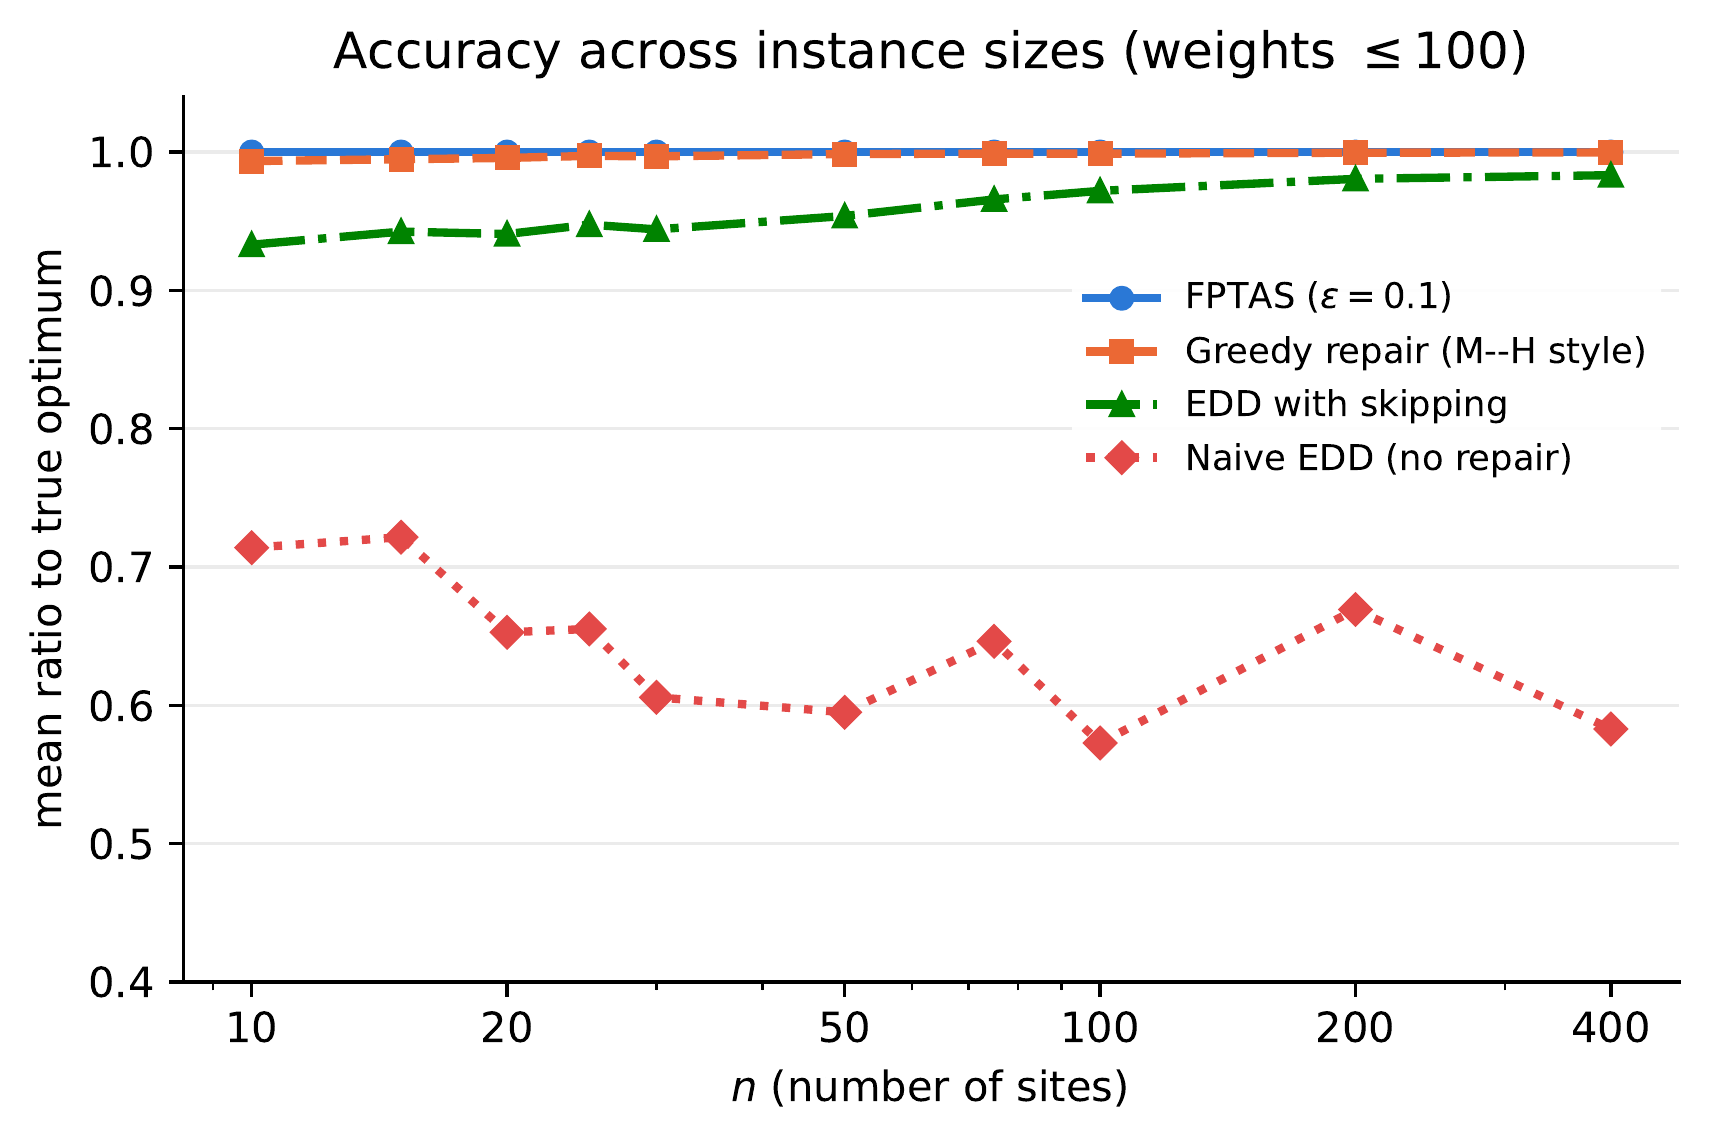
\includegraphics[width=0.72\textwidth]{accuracy_vs_n.png}
\caption{Table~\ref{tab:illustration} plotted. The FPTAS and greedy
repair sit at $1.0$; EDD with skipping improves slowly with $n$; naive
EDD fluctuates around $0.6$ with no trend and, on individual instances,
captures only a few percent of the optimum.}\label{fig:accuracy}
\end{figure}

The FPTAS recovers the optimum on every instance, but this is
\emph{not} evidence about the approximation scheme. With weights at most
$100$ the scaling factor $K=\max(1,\epsilon w_{\max}/n)$ equals $1$ for
$\epsilon=0.1$ at every $n\ge15$ and for $\epsilon=0.2$ at every
$n\ge25$ (last row of Table~\ref{tab:illustration}), so no rounding
takes place and the FPTAS coincides with the exact value-indexed
dynamic program; a ratio of $1.000$ is then guaranteed, not
informative. The next subsection therefore uses weights large enough
that the rounding is active. Among the heuristics, the greedy repair
captures $99.3$--$100\%$ of the optimum on average but has a worst
ratio of $0.93$ at $n=10$, consistent with its having no guarantee
(Proposition~\ref{prop:repair}); naive EDD shows no trend with $n$, as
a rule that never reconsiders would not, though a worst-case result such
as Proposition~\ref{prop:naive} does not by itself predict average
behavior on random instances.

\subsection{The FPTAS with active scaling}\label{sec:scaling}

We now take weights up to $10^6$ with $p_i\le20$, so that the
time-indexed exact dynamic program stays cheap (its table depends on
$P$, not on the weights) and serves as the reference, while the
FPTAS's scale factor $K$ is in the hundreds to thousands. Three
families are used, with $n=100$ and $30$ instances per $\epsilon$ for
the first two. \emph{Random:} weights uniform on $\{1,\dots,10^6\}$.
\emph{Strongly correlated:} a common deadline and $w_i=1000p_i+500$ with
$p_i$ up to $1000$, the hard family for knapsack-type schemes
(\citealp{hejl2022} study this regime for exact algorithms).
\emph{Adversarial:} the first family of Proposition~\ref{prop:tight}, with
one dominant site and $n-1$ sites just below the scaling granule. This
column is a single deterministic instance, not an empirical worst case: its
entries equal the closed form $n/(n+(n-1)\epsilon)$ of the proposition for
$n=100$ and large $M$. For each, Table~\ref{tab:scaling} reports the worst ratio over the instances
for Algorithm~\ref{alg:fptas} as stated and, for the adversarial family,
with the completion step of Remark~\ref{rem:completion}.

\begin{table}[h]
\caption{FPTAS accuracy with active scaling ($n=100$, $p_i\le20$ or as
stated). Entries are the \emph{worst} ratio to the optimum over the
instances of each family ($30$ per $\epsilon$ for the first two). ``Share $<1$''
is the fraction of random instances on which the FPTAS was not exactly
optimal. Every entry respects the guarantee $1-\epsilon$.}\label{tab:scaling}
\small
\begin{tabular}{@{}lcccccc@{}}
\toprule
$\epsilon$ & $1-\epsilon$ & Random & Share $<1$ & Str.\ corr. & Adv.\ (analytic) & Adv.\ + completion \\
\midrule
0.50 & 0.50 & 0.9998 & 0.30 & 0.9993 & 0.669 & 1.000 \\
0.30 & 0.70 & 0.99996 & 0.10 & 0.9994 & 0.771 & 1.000 \\
0.20 & 0.80 & 0.99996 & 0.10 & 0.9994 & 0.835 & 1.000 \\
0.10 & 0.90 & 0.99999 & 0.03 & 0.9996 & 0.910 & 1.000 \\
0.05 & 0.95 & 1.00000 & 0.00 & 0.9996 & 0.953 & 1.000 \\
\bottomrule
\end{tabular}
\end{table}

\begin{table}[h]
\caption{Cost of the FPTAS as $\epsilon$ shrinks (random weights up to
$10^6$, $n=100$): mean scaling factor $K$, mean number of dynamic-program
cells, and mean wall-clock time. A value-indexed exact table would need
about $5\times10^{7}$ columns per row at these weights, against the
$10^{4}$--$10^{5}$ used here.}\label{tab:epscost}
\small
\begin{tabular}{@{}lccccc@{}}
\toprule
$\epsilon$ & 0.50 & 0.30 & 0.20 & 0.10 & 0.05 \\
\midrule
mean $K$ & 4{,}996 & 2{,}997 & 1{,}998 & 999 & 500 \\
cells ($\times10^6$) & 0.99 & 1.65 & 2.47 & 4.95 & 9.90 \\
time (ms) & 3.8 & 5.9 & 8.1 & 18.3 & 47.8 \\
\bottomrule
\end{tabular}
\end{table}

\begin{figure}[h]
\centering
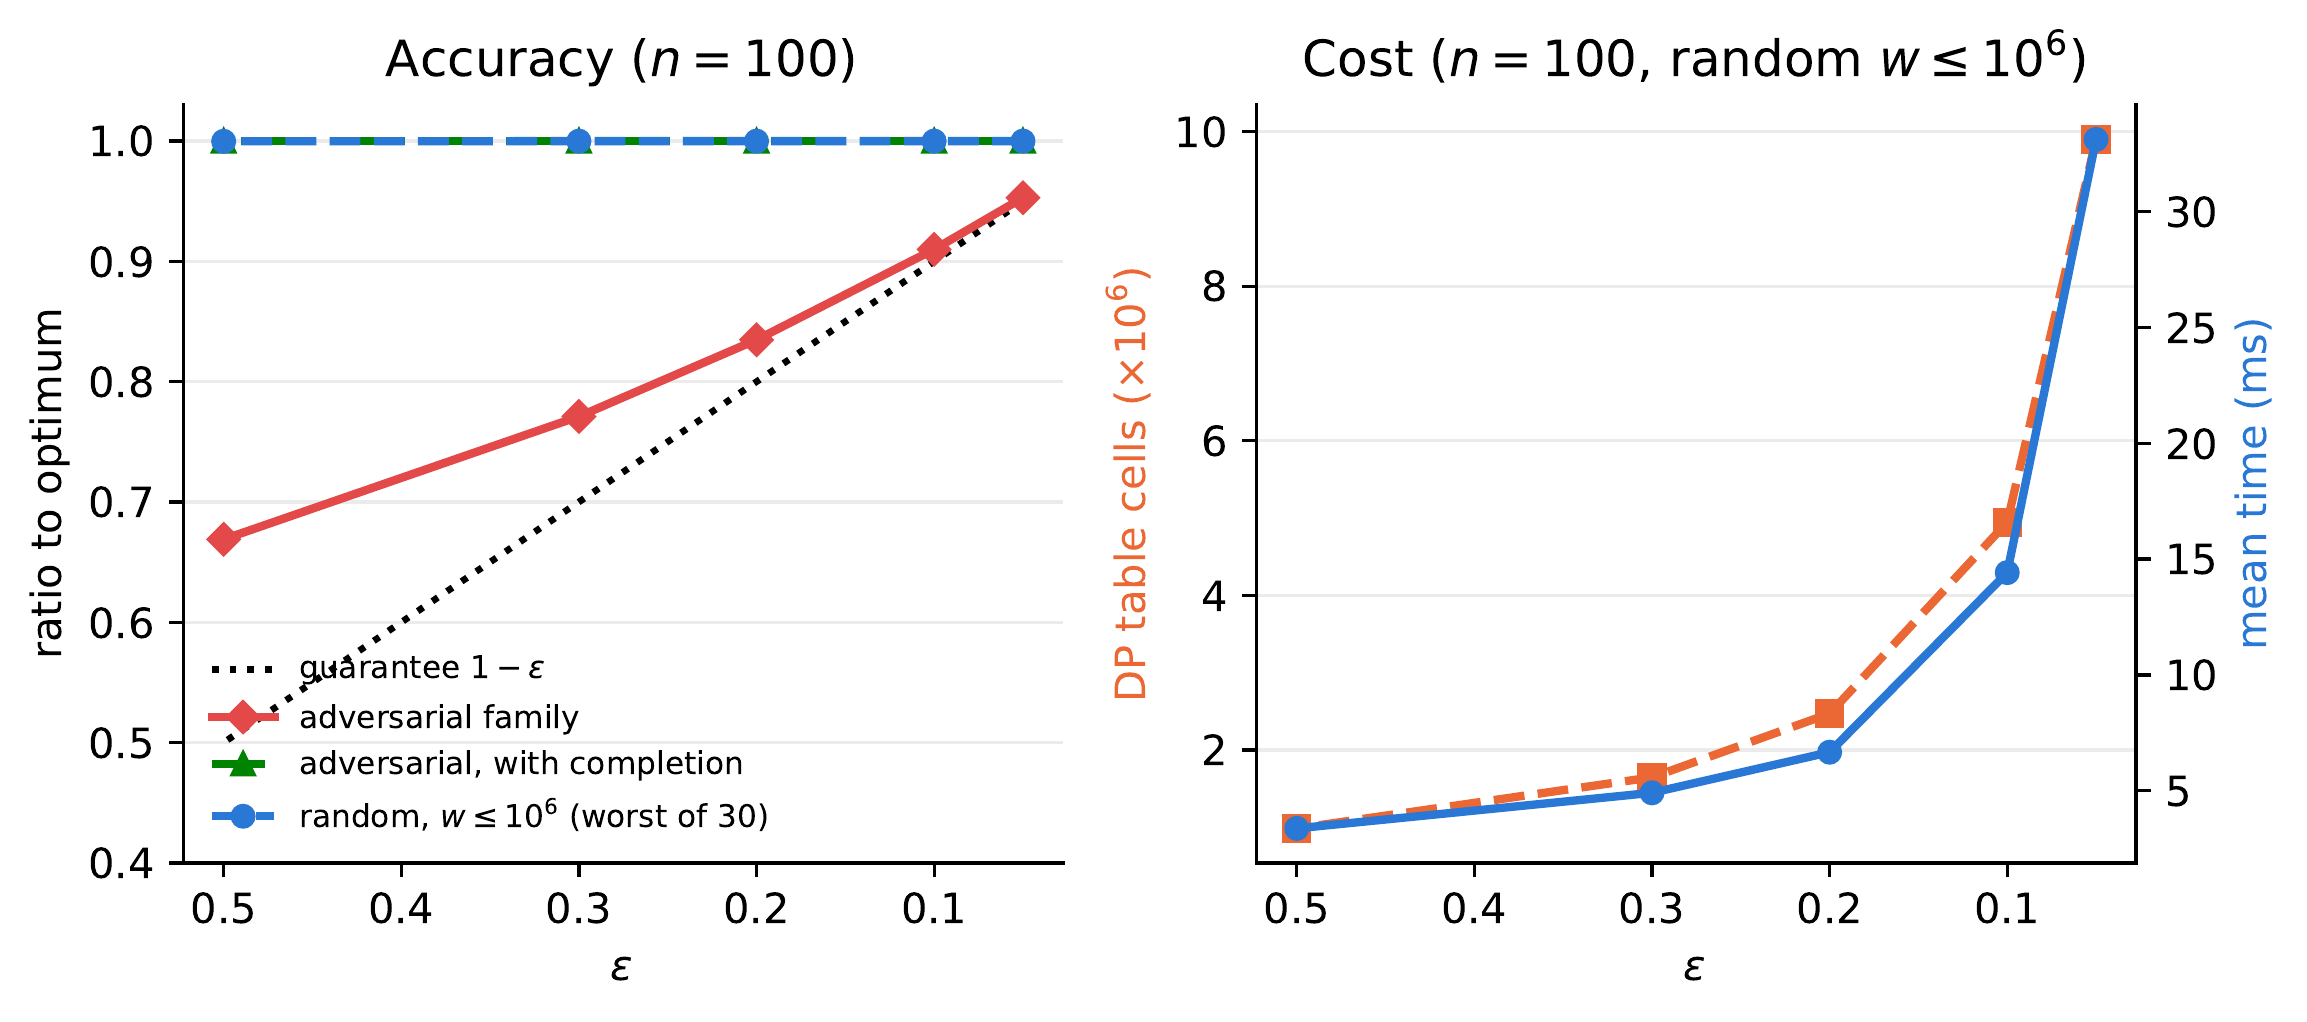
\includegraphics[width=0.95\textwidth]{epsilon_sensitivity.png}
\caption{Tables~\ref{tab:scaling} and~\ref{tab:epscost} plotted. Left:
the worst ratio on the adversarial family tracks the guarantee
$1-\epsilon$ (it stays above it and, as Proposition~\ref{prop:tight}
shows, approaches $1/(1+\epsilon)$); on random instances the FPTAS is
essentially exact, and the completion step makes the adversarial
family exact. Right: cost grows in proportion to $1/\epsilon$, as the
$O(n^3/\epsilon)$ bound says.}\label{fig:epsilon}
\end{figure}

Two things are visible. First, on random and on strongly correlated
instances the FPTAS is nearly exact even at $\epsilon=0.5$ (worst ratio
$0.9993$), far above its guarantee: the bound $\epsilon w_{\max}$
charges every selected site a full rounding error $K$ and compares the
total to $w_{\max}$, whereas on these instances the optimum contains
many sites and $W^\ast\gg w_{\max}$. This is why the ratio is close to
$1$, and it is the answer to the question of why accuracy is near $1$ in
all earlier tables. Second, the guarantee is \emph{not} vacuous: on the
adversarial family, which Proposition~\ref{prop:tight} shows is the
worst case, the ratio falls to $0.669$ at $\epsilon=0.5$ and follows
the guarantee as $\epsilon$ shrinks, so a planner who needs a worst-case
bound cannot do better than an $\epsilon$-dependent cost. The inexpensive
completion step removes this failure on the family. Cost grows in
proportion to $1/\epsilon$ (Table~\ref{tab:epscost}), as predicted, and
is independent of $P$ (next subsection).

\subsection{Runtime: time-indexed versus value-indexed}\label{sec:runtime}

Theorem~\ref{thm:dp}'s dynamic program runs in $O(nP)$ time, with
$P=\sum_ip_i$ exponential in the input's bit length; the FPTAS's table
does not depend on $P$. To see this, fix $n=40$, $\epsilon=0.1$, draw
weights up to $10^6$ (so the scaling is active at every setting), vary
the range $p_{\max}$ from which dispatch times are drawn, and time both
algorithms on $5$ random instances per setting.

\begin{table}[h]
\caption{Mean wall-clock time (milliseconds), $n=40$, $\epsilon=0.1$,
weights up to $10^6$, over 5 random instances per row, as $p_{\max}$
grows (so $P$ grows roughly proportionally).}\label{tab:runtime}
\begin{tabular}{@{}lccccc@{}}
\toprule
$p_{\max}$ & 50 & 200 & 800 & 3{,}200 & 12{,}800 \\
\midrule
Exact DP (Theorem~\ref{thm:dp}) & 0.54 & 1.26 & 3.57 & 14.1 & 82.8 \\
FPTAS (Theorem~\ref{thm:fptas}) & 1.39 & 1.64 & 1.86 & 1.88 & 1.88 \\
\bottomrule
\end{tabular}
\end{table}

\begin{figure}[h]
\centering
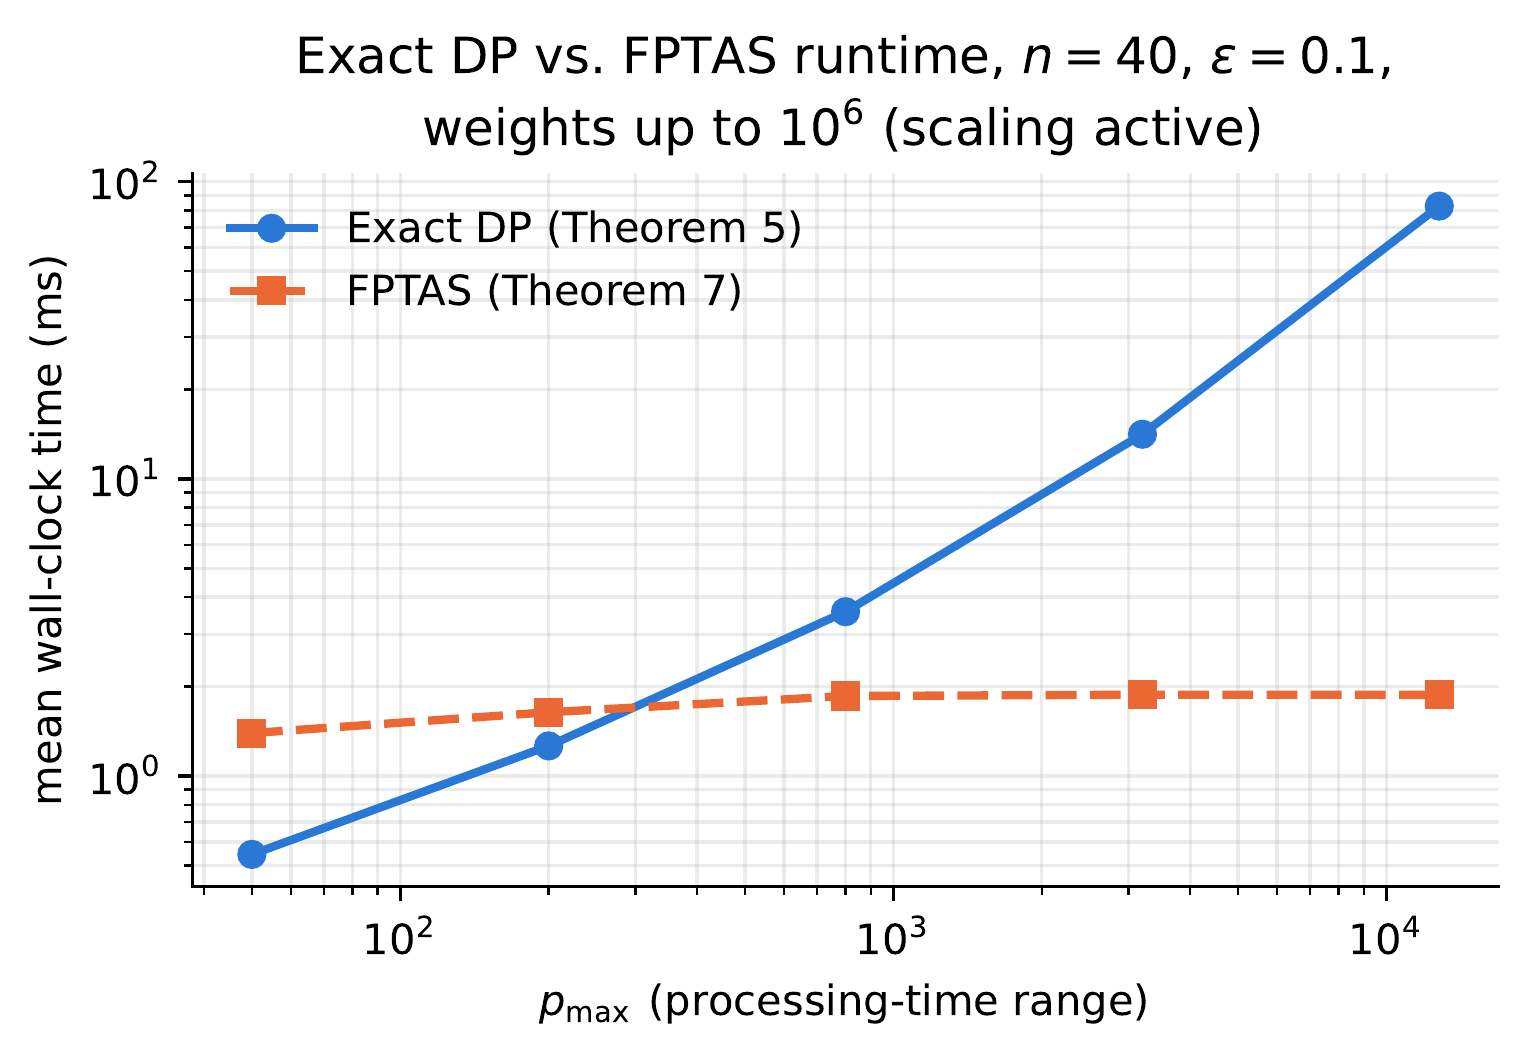
\includegraphics[width=0.68\textwidth]{runtime_scaling.png}
\caption{Table~\ref{tab:runtime} on log-log axes: the exact DP's time
grows with $p_{\max}$ (roughly linearly or slightly faster once the
fixed overhead is exceeded), while the FPTAS's stays flat.}\label{fig:runtime}
\end{figure}

The exact dynamic program grows about $150$-fold as $p_{\max}$ grows
$256$-fold (the smallest settings are dominated by fixed overhead),
whereas the FPTAS is flat up to noise.
At the smallest $p_{\max}$ the exact program is faster in absolute
terms, a reminder that an approximation scheme pays off only when the
numerical magnitude is large. We stress that this comparison is between
a time-indexed and a value-indexed table, and that the dependence on the
weights has simply moved: a value-indexed \emph{exact} program would
depend on $\sum_iw_i$ in the same way.

\subsection{Comparison with a general-purpose solver}\label{sec:mip}

As an independent baseline we solve the same instances with a
general-purpose mixed-integer solver (HiGHS, through
\texttt{scipy.optimize.milp}) on the subset formulation: binary $x_i$,
sites in deadline order, and for every $i$ the constraint
$\sum_{j\le i}p_jx_j+(P-d_i)x_i\le P$, which by Lemma~\ref{lem:edd}
expresses feasibility, maximizing $\sum_iw_ix_i$. On $10$ random
instances per size ($p_i\le20$, $w_i\le100$) both methods return the same
optimum on every instance, and the dynamic program is much cheaper:
Table~\ref{tab:mip}. The comparison is not meant to dismiss MIP
technology; it shows that for this structure the dynamic program of
Theorem~\ref{thm:dp} is the right tool when dispatch times are small
integers, and it provides an independent check of the optima.

\begin{table}[h]
\caption{Mean wall-clock time (milliseconds) of the exact dynamic program
and of HiGHS on the subset MIP, $10$ random instances per size; the last
row gives the slowest MIP solve. Optima agree on all $40$
instances.}\label{tab:mip}
\begin{tabular}{@{}lcccc@{}}
\toprule
$n$ & 20 & 50 & 100 & 200 \\
\midrule
Exact DP & 0.29 & 0.78 & 1.47 & 3.49 \\
HiGHS (MIP) & 55.3 & 13.8 & 22.7 & 146.1 \\
slowest MIP solve & 514 & 49 & 48 & 434 \\
\bottomrule
\end{tabular}
\end{table}

\subsection{Robustness to the instance-generation regime}\label{sec:robust}

To check that the pattern of Table~\ref{tab:illustration} is not an
artifact of the generator we repeat the comparison at $n=30$ ($20$
instances each) under heavy-tailed weights (exponential, mean $20$) and
tight deadlines (the horizon narrowed to $0.5\sum_ip_i$).

\begin{table}[h]
\caption{Mean ratio to the true optimum under two alternative
instance-generation regimes, $n=30$, 20 random instances per row.
``Repair'' is the greedy repair of Algorithm~\ref{alg:repair}; ``Skip'' is
EDD with skipping; the FPTAS uses $\epsilon=0.1$.}\label{tab:robustness}
\begin{tabular}{@{}lcccc@{}}
\toprule
Regime & FPTAS & Repair & Skip & Naive EDD \\
\midrule
Heavy-tailed weights & 1.000 & 0.999 & 0.944 & 0.537 \\
Tight deadlines ($0.5\times$ horizon) & 1.000 & 0.988 & 0.799 & 0.125 \\
\bottomrule
\end{tabular}
\end{table}

The greedy repair is essentially unaffected and EDD with skipping
degrades under tight deadlines, where there is less slack to absorb a
poor early commitment; naive EDD collapses to $12.5\%$ of the optimum,
largely because it also wastes time on sites that are already late.
(As in Section~\ref{sec:acc}, the FPTAS entries are $1.000$ partly
because the scaling is vacuous at weights $\le100$.)

\subsection{A real-world illustration: the 2018 Camp Fire}\label{sec:campfire}

The instances above are synthetic by design: MWHED has no benchmark set,
and the experiments need controllable distributions. To ground the model's
scale in a real event we build one small instance from public records of
the 2018 Camp Fire (Butte County, California), the deadliest wildfire in
California history (85 civilian fatalities and 18{,}804 structures
destroyed, according to the NIST reconstruction cited below). We separate
real, documented inputs from disclosed modelling assumptions, and we
present the case as an \emph{illustration of the model and of its
sensitivity}, not as an operational recommendation or a reconstruction of
what any crew could have done.

\textbf{Documented inputs.} Every hazard-arrival time is a clock time
documented in the National Institute of Standards and Technology (NIST)
reconstruction of the fire's progression \citep{nist2021campfire}; none is
extrapolated. For each of four real communities in the fire's path we use
the earliest documented event of the kind NIST reports for it: the first
structures burning and spot fires igniting in \emph{Concow} (07:25 on
8~November), the first spot fires arriving in \emph{Paradise} (07:44; the
detailed sections of the report put the first 911 call about a Paradise
spot fire at 07:49, which lies inside the sensitivity range below), spot
fires in Old Magalia, the earliest-affected part of \emph{Magalia}
(08:40; most of Magalia burned much later), and the fire running through
\emph{Yankee Hill}, documented as ``well established'' at 08:40 on
9~November, about a day after ignition and therefore an almost
unconstraining deadline. The events are therefore not identical across
communities, which is a limitation of the data, not of the model; the
documentation is also uneven across communities, and Yankee Hill's event
is an upper bound on the fire's arrival there (the instance is in effect
a three-site one, as Yankee Hill's deadline never binds).
The weights are the 2010 U.S.\ Census populations (the last count before
the fire; later counts reflect the aftermath, and the NIST report quotes
different, survey-based figures): Paradise $26{,}218$, Magalia
$11{,}310$, Concow $710$, Yankee Hill $333$. Community coordinates are
their published centroids, and the depot (Oroville, CA) is a modelling
choice.

\textbf{Disclosed modelling assumptions.} (i) $p_i$ is twice the
great-circle distance between the depot and site $i$ (a lower bound on
road distance), divided by an assumed average response speed; we report
$50$~km/h (conservative, winding mountain roads) and $80$~km/h
(optimistic), and Table~\ref{tab:campfire-route} varies the road factor.
(ii) Time zero is the initial dispatch time in NIST's dispatch log,
06:31 on 8~November (NIST's own estimate of ignition is about 06:20, and
the first 911 call is at 06:25); the crew leaves at time zero (the dispatch to the fire's origin, not a
decision to defend these communities, so this is optimistic), and the
sensitivity analysis adds a departure delay, which only postpones it. (iii) The \emph{arrival
reading} of Remark~\ref{rem:reading} is used: a site is
\emph{protected} if the crew \emph{arrives} before the documented event,
so the MWHED deadline is $d_i=d_i^{\mathrm{haz}}+p_i/2$. ``Protected''
means arrival only: the model has no on-site service time (which would
simply add to $p_i$) and no notion of what protection achieves.
Table~\ref{tab:campfire} gives the instance.

\begin{table}[h]
\caption{The Camp Fire instance. $d^{\mathrm{haz}}$ is the documented
event time in minutes after time zero (06:31); $p_i$ is the round-trip
occupancy from the Oroville depot at the two response speeds; the MWHED
deadline under the arrival reading is $d_i=d^{\mathrm{haz}}+p_i/2$
(rounded, halves to the nearest even integer); $w_i$ is the 2010 census
population.}\label{tab:campfire}
\small
\begin{tabular}{@{}lcccccc@{}}
\toprule
Site & $d^{\mathrm{haz}}$ & $p_i$ (50) & $p_i$ (80) & $d_i$ (50) & $d_i$ (80) & $w_i$ \\
\midrule
Concow & 54 & 63 & 39 & 86 & 74 & 710 \\
Paradise & 73 & 70 & 44 & 108 & 95 & 26{,}218 \\
Magalia & 129 & 89 & 55 & 174 & 156 & 11{,}310 \\
Yankee Hill & 1{,}569 & 54 & 34 & 1{,}596 & 1{,}586 & 333 \\
\bottomrule
\end{tabular}
\end{table}

\begin{figure}[h]
\centering
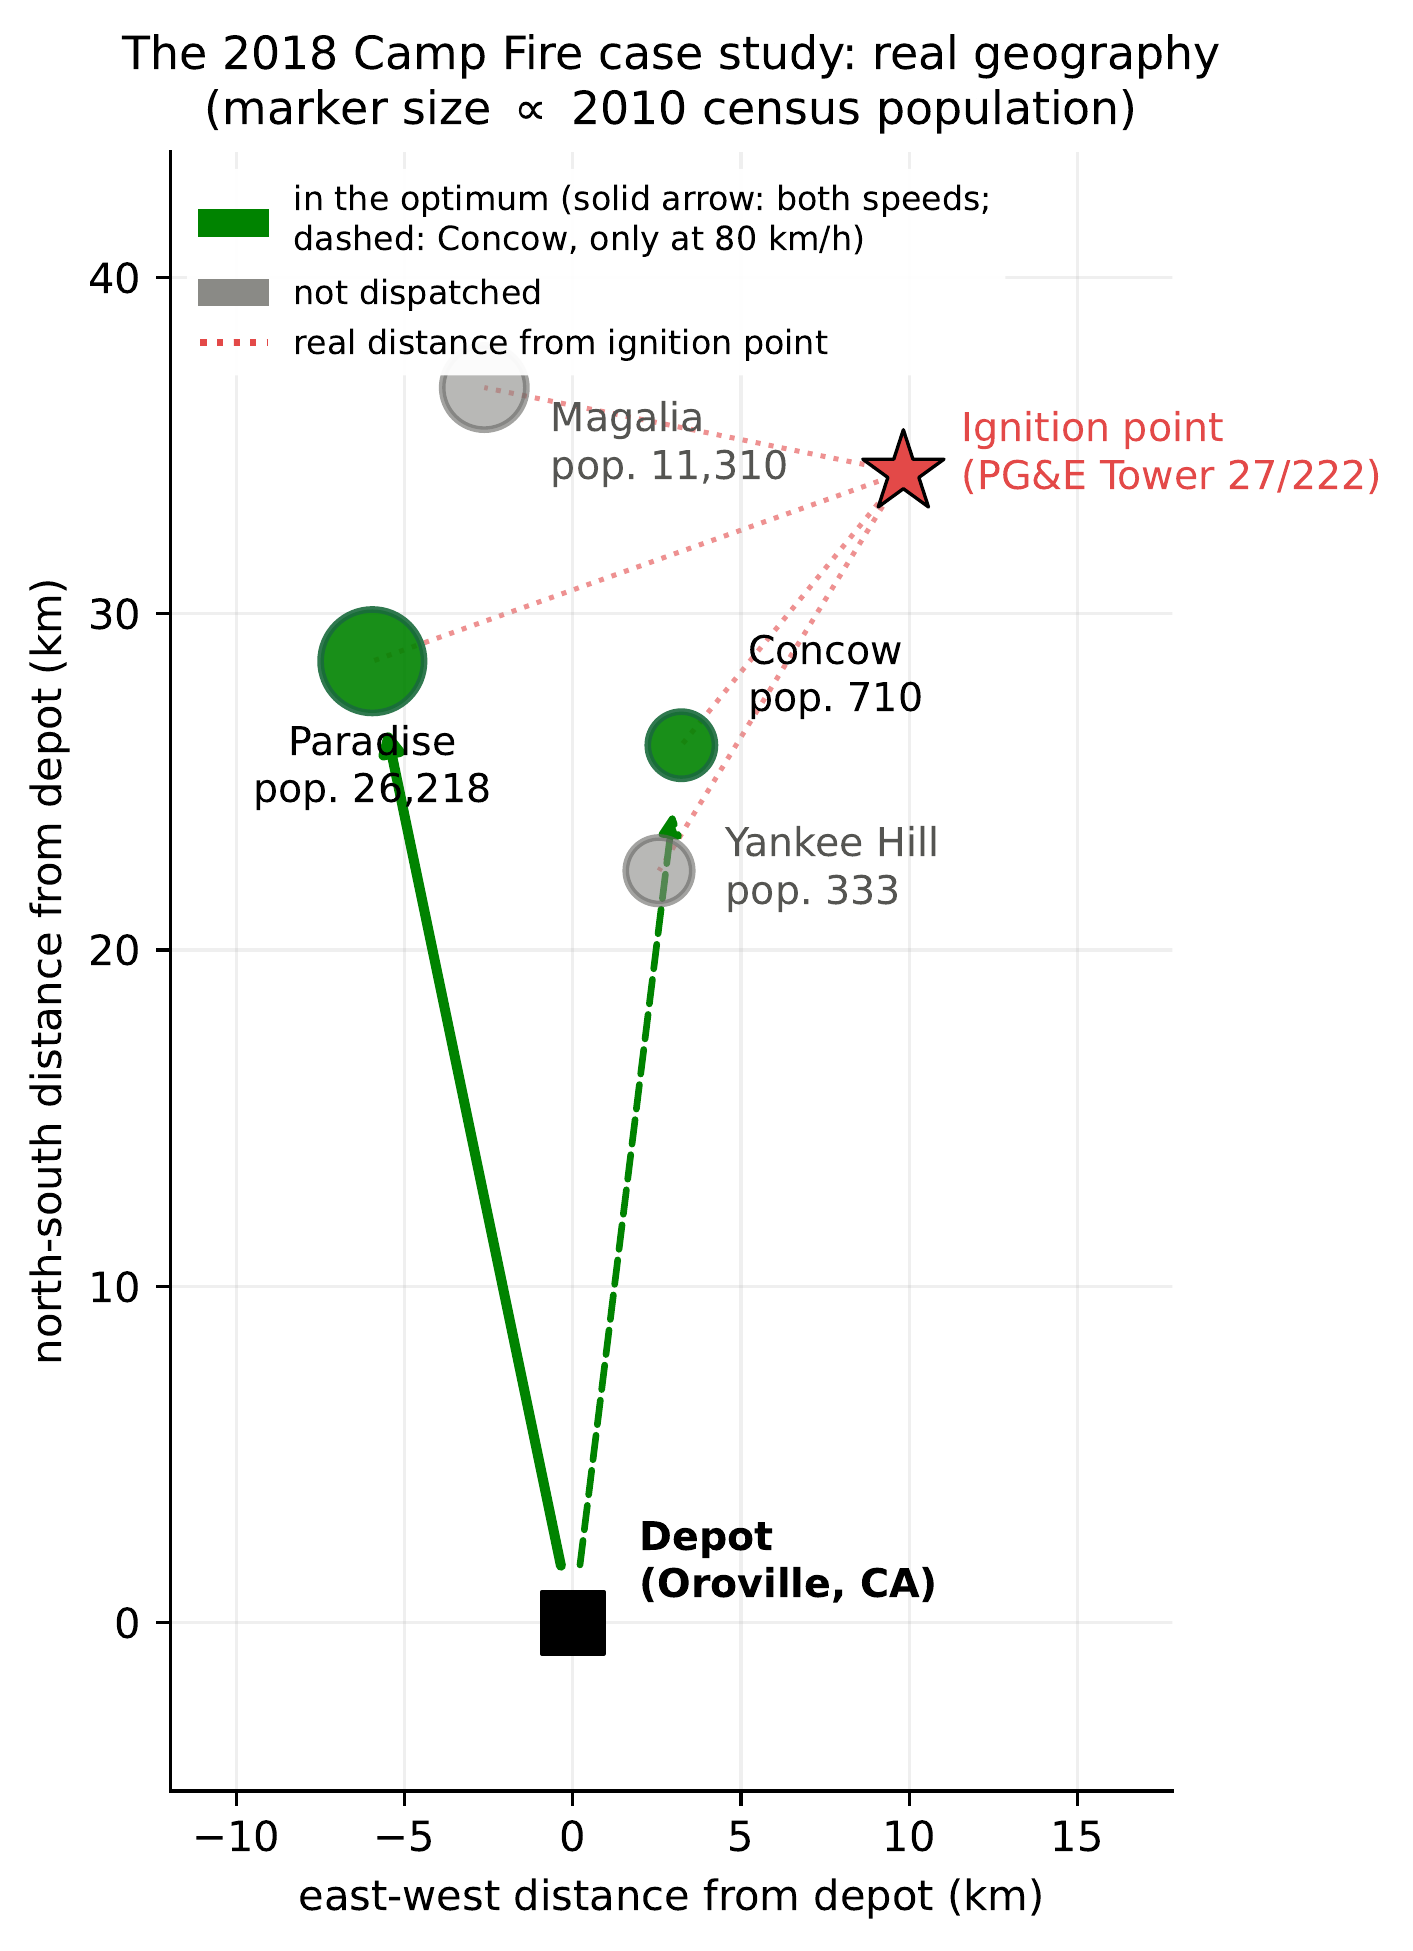
\includegraphics[width=0.75\textwidth]{campfire_map.png}
\caption{The geography behind Table~\ref{tab:campfire}: the depot, the
fire's origin point as given by NIST, and the four communities, plotted
from their published coordinates, with the hazard time of each. Solid
gray lines are the depot round trips of the MWHED model; the dashed
arrows are the chained route of Table~\ref{tab:campfire-route}. Green
markers are the sites of the $50$~km/h depot-spoke optimum of
Table~\ref{tab:campfire-results}.}\label{fig:campfire-map}
\end{figure}

\begin{table}[h]
\caption{On-time weight (population) of each algorithm on the Camp Fire
instance, arrival reading; the sites served are in parentheses. The total
weight is $38{,}571$. C, P, M, Y denote Concow, Paradise, Magalia, Yankee
Hill.}\label{tab:campfire-results}
\small
\begin{tabular}{@{}lcc@{}}
\toprule
 & $50$~km/h & $80$~km/h \\
\midrule
Exact optimum (Thm.~\ref{thm:dp}) & 37{,}861 (P, M, Y) & 38{,}571 (all) \\
FPTAS, $\epsilon=0.1$ (Thm.~\ref{thm:fptas}) & 37{,}528 (P, M) & 38{,}238 (C, P, M) \\
Greedy repair & 37{,}861 & 38{,}571 \\
EDD with skipping & 12{,}353 (C, M, Y) & 38{,}571 \\
Naive EDD & 1{,}043 (C, Y) & 38{,}571 \\
\bottomrule
\end{tabular}
\end{table}

\textbf{Results.} At $80$~km/h the trips are short enough that every
algorithm, even naive deadline order, serves all four communities. At
$50$~km/h the picture changes: Concow's early deadline (86 minutes) and
Paradise's (108) cannot both be met, and the optimum gives up Concow
(weight $710$) to protect Paradise, Magalia and Yankee Hill, for
$37{,}861$ of the $38{,}571$ total. Deadline-order rules go to Concow
first because its deadline is earliest, and they pay for it: naive EDD
reaches an on-time weight of only $1{,}043$, and EDD with skipping $12{,}353$, a third
of the optimum, because serving Concow makes Paradise late. The greedy
repair finds the optimum on both speeds, and the FPTAS with $\epsilon=0.1$
returns $99.1\%$ of the optimum at $50$~km/h: Yankee Hill's weight $333$
is below the scaling granule $K\approx655$ and is dropped, which is
exactly the zero-scaled-site loss of Remark~\ref{rem:completion}
(re-inserting it recovers the optimum). Under the stricter \emph{return
reading} (the crew must be back before the fire arrives) the answer
changes: at $50$~km/h Concow is individually infeasible (round trip of
$63$ minutes against an arrival minute of $54$), the optimum is Paradise
and Yankee Hill ($26{,}551$), and Magalia's $11{,}310$ is lost; this is
why Remark~\ref{rem:reading} asks the user to state the reading.

\textbf{The round-trip premise on this geography.} The four communities
are $4$--$15$~km apart, against depot distances of $22$--$37$~km, so the
depot-spoke model is far from the geometry. By
Proposition~\ref{prop:spoke} it is conservative; Table~\ref{tab:campfire-route}
measures by how much, comparing the spoke optimum with the optimum of a
chained route (direct travel between consecutive sites, great-circle
distance times a road factor $\rho$, exhaustive over all ordered subsets).
With $\rho=1$ the chained route protects all four communities at both
speeds; at $50$~km/h the spoke model loses Concow, weight $710$. With
road factors $1.3$ and $1.6$ the spoke model loses more, because it
charges $\rho$ on every round trip while the hazard times stay fixed
(Paradise remains in the optimum), whereas the chained route still
protects all four. For this event the depot-spoke optimum is therefore a
safe but pessimistic plan, and the structural findings below should be read
as findings about the \emph{model}, to be confirmed on a routing model
before any operational use.

\begin{table}[h]
\caption{Depot-spoke optimum (the MWHED model) versus the optimum of a
chained route, by response speed and road factor $\rho$ (arrival reading,
protected weight out of $38{,}571$).}\label{tab:campfire-route}
\small
\begin{tabular}{@{}lcccc@{}}
\toprule
 & \multicolumn{2}{c}{spoke (MWHED)} & \multicolumn{2}{c}{chained route} \\
road factor $\rho$ & $50$ & $80$ & $50$ & $80$ \\
\midrule
$1.0$ & 37{,}861 & 38{,}571 & 38{,}571 & 38{,}571 \\
$1.3$ & 26{,}551 & 37{,}861 & 38{,}571 & 38{,}571 \\
$1.6$ & 26{,}551 & 37{,}861 & 38{,}571 & 38{,}571 \\
\bottomrule
\end{tabular}
\end{table}

\textbf{Sensitivity to the uncertain inputs.} The inputs are uncertain in
several ways: the response speed, the documented event times (each is an
estimate from observations, and the events differ in kind across
communities), and the dispatch delay. We draw $20{,}000$ scenarios with
the speed uniform on $[40,90]$ km/h, the event times of Concow and
Paradise scaled by independent factors uniform on $[0.85,1.15]$, those of
Magalia and Yankee Hill (whose events are less sharply defined) on
$[0.70,1.30]$, and a departure delay uniform on $[0,20]$ minutes, and
solve each exactly. We also run a \emph{correlated} variant in which one
common factor, uniform on $[0.70,1.30]$, scales all event times (a
systematic bias of the fire reconstruction), with a small independent
factor on $[0.95,1.05]$ per site. Standard errors of the reported shares
are at most $0.4$ percentage points.

\emph{Protocol.} A plan is a fixed visiting sequence in the order Concow,
Paradise, Magalia, Yankee Hill, restricted to its sites; every visit is a
round trip, and a site that Assumption~\ref{as:feasible} deletes in a
draw is skipped (so a hopeless first visit does not consume time). The
\emph{retained share} of a plan in a draw is its protected weight divided
by the optimum of that draw. If instead every site of the plan is visited
even when hopeless, the mean retained share of the nominal plan drops from
$0.319$ to $0.289$; we report the first protocol.

Paradise is in the optimum in all draws of the independent variant and in
$99.2\%$ of the correlated one; at $50$~km/h it leaves the optimum only if
its weight falls below $710$, Concow's. The decision is in effect a single
binary conflict, whether to visit Concow ($710$) before Paradise
($26{,}218$): Yankee Hill's event is a day away and never binds, and
Magalia rarely does. The optimal set is Paradise, Magalia and Yankee Hill
in $63.1\%$ of the independent draws, Paradise with Yankee Hill in
$20.7\%$ and all four communities in $16.2\%$.

The nominal plan depends on the nominal speed. The optimum of the nominal
instance (no delay) includes Concow only from about $68$~km/h upward, since
the round trips to Concow and Paradise must both fit before Paradise's
deadline. The plan that is optimal at $80$~km/h, an optimistic corner of
the speed range, visits Concow first and is fully on time in only
$16.2\%$ of the draws, retaining on average $31.9\%$ of the drawn optimum
(fifth percentile $2.8\%$), because a delay or a slower road lets the
Concow visit make Paradise late; Paradise has only $12$ minutes of slack.
The plans that are optimal at $65$ or $50$~km/h, and the sample-average
plan described next, all drop Concow: Paradise, Magalia and Yankee Hill.
That plan is fully on time in $79.3\%$ of the draws and retains $99.7\%$
of the drawn optimum on average (fifth percentile $98.2\%$); since Concow
carries $1.8\%$ of the total weight, any plan that drops it retains at
least $98.2\%$ of an optimum that includes it. The \emph{sample-average
plan} is the subset (in the same visiting order) with the largest average
protected weight over an independent sample of $2{,}000$ draws; it
coincides with the conservative-speed optimum, so here the scenario
sample confirms what a conservative nominal speed already gives, and its
value would lie in problems where the right nominal is not obvious. Under
correlated errors the figures are $26.0\%$ and $37.2\%$ for the
$80$~km/h plan and $79.1\%$ and $99.5\%$ for the others. Finally, a
chained route with road factor $1.0$ (resp.\ $1.3$) protects all four
communities in $96.1\%$ (resp.\ $79.5\%$) of the independent draws.

\textbf{What the case study does and does not show.} The finding is
conditional and modest: in this model the exact optimum inherits whatever
nominal speed (that is, slack) is assumed. When the assumption is
optimistic, the plan spends Paradise's slack on a small community and
fails under timing errors; planning for a conservative speed removes the
failure at a cost of at most the small community's weight. This is a
property of the depot-spoke model, which Table~\ref{tab:campfire-route}
shows to be a poor fit for this geography, and a scenario formulation
(Section~\ref{sec:disc-stochastic}) is the natural way to make such
choices. The study does not show what a real crew should have done: the
model ignores on-site service, road closures, evacuation (the main
protection in this event) and the fact that the dispatch itself changes
the fire. The objective is also a choice with ethical content. Weighting
by population and conceding the sites with the least weight is
utilitarian; a planner may instead require a minimum protection level for
every community, or weight by vulnerability. A set of sites that must be
protected can be forced into the plan, within the same model, by adding a
constant larger than the total weight to their weights (provided each is
individually feasible); proportional-fairness constraints generally break
the knapsack structure. We therefore treat the numbers above as a worked
illustration of the model and its sensitivity, on a single event with
four sites, and as nothing more.

% ══════════════════════════════════════════════════════════════════
\section{Discussion and extensions}\label{sec:discussion}

Section~\ref{sec:theory} treats the single-depot, single-vehicle,
deterministic-deadline case. Three natural
directions relax one assumption at a time; we discuss, for each, what
carries over from our analysis and what specifically breaks, rather
than simply listing them as unexplored future work.

\subsection{Multiple depots or vehicles}\label{sec:disc-multi}

Suppose $m>1$ vehicles are available, each serving its own sequence of
round trips, as in MWHED-$m$ of Section~\ref{sec:equalp}. Four facts
describe what changes.

\emph{Hardness persists for every fixed $m$.} Take a common-deadline
instance with deadline $D$ and total weight $\Omega=\sum_iw_i$ (the
hard instances of Theorem~\ref{thm:hardness}) and add $m-1$ ``blocker''
sites with $p=d=D$ and weight $\Omega+1$. A blocker occupies a vehicle
for all of $[0,D]$: if anything is served on that vehicle before it, the
blocker is late, and if anything is served after it, that site is late.
So each served blocker uses a vehicle exclusively, dropping a blocker
costs $\Omega+1$ and can free a vehicle worth at most $\Omega$, and an
optimum serves all $m-1$ blockers and solves the original instance on the
one remaining vehicle. Hence MWHED-$m$ is NP-hard for every fixed $m$.
(Simply adding idle vehicles to an instance would not do: extra vehicles
can serve sites, which changes the problem.)

\emph{The exact dynamic program grows with $m$.} Theorem~\ref{thm:dp}'s
recursion extends by tracking a completion time per vehicle. Assign sites
in deadline order (Lemma~\ref{lem:edd}, applied on each vehicle) and let
$f(i,t_1,\dots,t_m)$ be the maximum on-time weight using sites
$1,\dots,i$ when vehicle $k$ has accumulated exactly $t_k$ occupancy;
site $i$ may be appended to any vehicle $k$ with $t_k\le d_i$,
\begin{multline*}
f(i,t_1,\dots,t_m)=\max\Bigl(f(i-1,t_1,\dots,t_m),\\
\max_{k:\,p_i\le t_k\le d_i}
\bigl(f(i-1,t_1,\dots,t_k-p_i,\dots,t_m)+w_i\bigr)\Bigr).
\end{multline*}
The table has $O(nP^m)$ cells, pseudo-polynomial for fixed $m$ but with
an exponent that grows with the number of vehicles. Whether this is
unavoidable is open here; the parallel-machine scheduling literature
treats the problem as considerably less settled than the single-machine
case \citep{lenstra1977}. We conjecture, but have not verified, that
value-scaling extends to an $m$-dimensional state.

\emph{Equal-size sites stay tractable, even for vehicles of different
speeds.} Theorem~\ref{thm:equalp} solves MWHED-$m$ with equal-size sites
in $O(m+n\log n)$ time for every $m$, identical vehicles or vehicles with
different dispatch times $p_v$. This is the multi-vehicle analogue of the
single-vehicle special case, and it holds without release dates.

\emph{Release dates are a different problem.} Theorem~\ref{thm:equalp}
assumes that every vehicle and every site is available from time~$0$.
\citet{heegermolter2025} show that the \emph{unweighted} problem on $m$
identical machines with equal processing times and release dates,
$P|r_j,p_j{=}p|\sum U_j$, is NP-hard and $W[2]$-hard parameterized by the
number of machines. Hence the tractability of
Theorem~\ref{thm:equalp} for an arbitrary number of identical vehicles
does not carry over to release dates (unless $\mathrm P=\mathrm{NP}$). That result does not
concern a single vehicle: for one machine, equal processing times,
weights and release dates are polynomial \citep{baptiste1999}. Release
dates have no counterpart in MWHED as defined here, since every vehicle
is at the depot at time $0$ and every site can be served from the start;
they would arise if sites become reachable, or crews available, only at
given times (for instance, a road cleared by a firebreak), and extending
the model in that direction for several vehicles is a natural open
problem.

\subsection{A relocating depot or growing-radius hazard}\label{sec:disc-relocate}

Definition~\ref{def:mwhed} takes each site's round-trip dispatch time
$p_i$ as a fixed constant, appropriate when the depot is stationary. If
the depot itself can relocate between dispatches---a mobile command
post following a fire line, for instance---$p_i$ becomes a function of
the depot's current position, which in turn depends on the dispatch
order already chosen. Lemma~\ref{lem:edd}'s exchange argument relies
critically on $p_i$ being order-independent (Section~\ref{sec:model}'s
observation that every visit is a self-contained round trip); with a
relocating depot this fails, and the problem acquires genuine routing
structure on top of its scheduling structure. We expect this variant to
be at least as hard as MWHED (it contains MWHED as the special case of
a depot that chooses not to move) and likely strictly harder, since the
order in which sites are visited now affects future dispatch costs, not
just which deadlines are met. Proposition~\ref{prop:spoke} bounds the
effect from one side: with a fixed depot and metric travel times,
allowing the crew to chain sites can only enlarge what it protects (a
hazard that cuts direct roads between sites while the depot spokes stay
open would break this), so the round-trip optimum is a safe
lower bound, and Table~\ref{tab:campfire-route} shows the gap can be large
when sites are clustered. A full routing model (orienteering or
deadline-TSP, Section~\ref{sec:related}) would remove the gap at the price
of losing the exact algorithms and guarantees of this paper.

It is worth being precise about what ``growing-radius hazard'' does
and does not already mean for a \emph{stationary} depot, since the two
relaxations named in this subsection's title are not the same
complication. If the hazard simply expands outward from a fixed origin
at a fixed, known rate, its arrival time at each site is already fully
captured by the deadline $d_i$ in Definition~\ref{def:mwhed}---this is
exactly the reduction described in Section~\ref{sec:intro}, and
requires no extension to our model at all. The genuine second
relaxation, distinct from a relocating depot, arises if the spreading
hazard itself degrades the road or access network the depot's vehicle
uses---for instance, a wildfire making a route impassable once it
crosses that route, or rising floodwater cutting off a bridge---so that
$p_i$ is not merely unknown but a function of \emph{when} site $i$ is
reached, since a later attempt may have to detour around
hazard-affected infrastructure that an earlier attempt would not have.
This again breaks Lemma~\ref{lem:edd}'s order-independence assumption,
but through the road network's degradation rather than the depot's own
movement, and the two effects would compound if both are present
simultaneously.

\subsection{Uncertain parameters}\label{sec:disc-stochastic}

Definition~\ref{def:mwhed} takes the dispatch times $p_i$, the
deadlines $d_i$ and the weights $w_i$ as known exactly. In practice
each is an estimate: arrival times come from a fire-spread, flood or
plume simulator and carry its forecast error; occupancies depend on road
conditions that the hazard itself may degrade; weights are proxies for
population or asset exposure. The optimal solutions and the structural
statements above are conditional on these inputs, and the case study of
Section~\ref{sec:campfire} shows that the nominal optimum can be brittle
under plausible perturbations. We discuss three ways to model the
uncertainty, and which of our results survive each.

\emph{Scenario-based (stochastic) models.} Let uncertain parameters
take values $\xi_s=(p^s,d^s,w^s)$ with probabilities $\pi_s$ for
$s=1,\dots,S$, and let the dispatch order $\sigma$ be chosen before the
scenario is revealed. The natural objective is the expected on-time
weight $\sum_s\pi_s\sum_iw_i^s\,\mathbb 1[C_i^s(\sigma)\le d_i^s]$,
which for $S=1$ is MWHED and is therefore NP-hard. Lemma~\ref{lem:edd}
holds scenario by scenario but not simultaneously: no single order sorts
all scenarios' deadlines, and the exchange argument fails. A small
example shows that sorting by expected deadline can be nearly twice as
bad as the optimum. Two sites with $p=1$: site $A$ with $w_A=1$ and
deadline $2$, and site $B$ with $w_B=10$ and a random deadline equal to
$1$ or $100$ with probability $\tfrac12$ each, so $\mathbb E[d_B]=50.5>
\mathbb E[d_A]=2$. Serving $A$ first (the expected-deadline order) gives
$1+10\cdot\tfrac12=6$; serving $B$ first gives $10+1=11$, because $B$'s
tight realization is avoidable only by acting immediately. This is the
setting of two-stage stochastic programming, in which a first-stage plan
is evaluated against scenario-dependent recourse; evacuation planning
under uncertain demand and network damage
\citep{wang2020evac} and facility location under disruptions
\citep{koca2023} are close relatives in the disaster-response
literature. A sample-average formulation of the expected-weight
objective is a mixed-integer program whose combinatorial core is
MWHED with scenario-dependent deadlines; a Benders-type decomposition by
scenario is natural, and exploiting Lemma~\ref{lem:edd} within a scenario
to generate cuts is, we believe, a promising direction that we have not
pursued.

\emph{Robust feasibility.} Feasibility of a set of sites is monotone in
the parameters: it is preserved when $d_i$ increases or $p_i$
decreases. A set that is on time for \emph{every} realization in a box
$[p_i^-,p_i^+]\times[d_i^-,d_i^+]$ is therefore exactly a feasible set
of the MWHED instance $(p^+,d^-,w)$, and every result above applies to
that worst-case instance. This is cheap but conservative; in the case
study the worst corner of the sampled ranges (slow roads, early arrival,
a $20$-minute delay) makes even Paradise individually infeasible, so
instance-wise robustness would return nothing. Chance-constrained or
scenario-averaged objectives are the useful formulations there.

\emph{Calibration and sensitivity.} Because the inputs are data-driven,
reporting how the optimum moves with them, as in
Section~\ref{sec:campfire}, is part of using the model. The case study
shows a practical pattern that scenario models would formalize: the
exact optimum of the nominal model inherits the assumed slack, so an
optimistic nominal speed can spend the slack of a dominant site on a small
one (retaining $31.9\%$ of the drawn optimum), whereas a conservative
nominal speed or a plan chosen against a sample of perturbed scenarios
retains $99.7\%$ (Section~\ref{sec:campfire}).

% ══════════════════════════════════════════════════════════════════
\section{Conclusion}\label{sec:conclusion}

We have studied Minimum Weighted Hazard-Exposure Dispatch, a scheduling
problem that arises whenever a single depot must choose a dispatch order
against a spreading hazard with site-specific arrival deadlines. The
problem is exactly the classical weighted on-time-jobs problem
$1\|\sum w_jU_j$ in transportation language; consequently its weak
NP-hardness, the pseudo-polynomial dynamic program, the approximation
scheme and the matroid greedy algorithm for equal-size sites (for any
number of vehicles, identical or not) are classical, and we have presented
them with complete, machine-checked proofs rather than as new techniques.
The classification of the homogeneous restrictions is an elementary
corollary, and not the natural tractability boundary of the scheduling
literature, where agreeable weights are the classical polynomial case.

What the dispatch setting adds is modest. Under the arrival reading of
the deadline, hardness persists when the hazard-arrival time is the same
at every site; the depot round-trip model is a conservative bound on a
chained route, which says when its premise is costly (clustered sites);
and the FPTAS has the guarantee
$\rho_{n,\epsilon}>1/(1+\epsilon)$, best possible for the scheme as
stated and sharper than the textbook $1-\epsilon$, which is not attained. Natural heuristics (deadline order
with or without skipping, a weighted greedy repair) have unbounded
worst-case ratio, although the greedy repair is within $1\%$ of the
optimum on random instances; a guarantee requires a rule that reconsiders
earlier commitments in light of both weights and dispatch times, and the
dynamic program and the FPTAS are two such rules, not the only ones.

The numerical study and the case study carry two lessons beyond the
theorems. The reading of the deadline (the crew must arrive before the
hazard, or return before it) changes the answer on the same data and must
be stated. And the optimum of a model with estimated inputs inherits the
assumed slack: on the Camp Fire instance, built from the hazard-arrival
times that NIST documents for each community, an optimistic nominal speed
yields a plan that places a small community ahead of the dominant one with
little slack and is fully on time in only $16\%$ of the perturbed
scenarios, whereas planning for a conservative speed (which a sample of
scenarios also finds) retains almost all of the optimum, in this model. The case
study is a single event with four sites, evaluated in a model that is
conservative about routing (Proposition~\ref{prop:spoke}); it
illustrates the model and does not support operational recommendations.
Section~\ref{sec:discussion} discusses how scenario-based and robust
formulations would capture the brittleness, and which parts of the
analysis survive: Lemma~\ref{lem:edd} holds within a scenario but not
across scenarios, which is what makes the stochastic version a genuinely
different problem. Natural next steps are a stochastic or
chance-constrained MWHED with a decomposition that uses the
earliest-deadline lemma within scenarios, a routing variant that chains
sites with deadline guarantees, release dates for several vehicles, and
approximation schemes for a fixed number of vehicles.

\begin{appendices}

\section{Exhaustive verification of the running example}\label{app:exhaustive}

Examples~\ref{ex:running}--\ref{ex:fptas} rely on
Example~\ref{ex:running}'s instance being small enough to check by
exhaustive search, not only by the dynamic program itself. Since
Lemma~\ref{lem:edd} lets us restrict to dispatching each candidate
subset $S$ in increasing-deadline order, Table~\ref{tab:exhaustive}
lists all $2^4=16$ subsets of Example~\ref{ex:running}'s four sites
($p=(2,3,1,4)$, $d=(4,6,2,9)$, $w=(5,8,3,10)$), each dispatched in that
order, together with its total dispatch time and feasibility. Every
feasible subset's weight is at most $23$, and $\{1,2,4\}$ attains it,
confirming $W^\ast=23$ independently of Algorithm~\ref{alg:exact}.

\begin{table}[h]
\caption{All $16$ subsets of Example~\ref{ex:running}'s running
instance, dispatched in increasing-deadline order. ``Sum $p$'' is the
subset's total dispatch time; a subset is feasible iff every member
completes on time in this order (Lemma~\ref{lem:edd}).}\label{tab:exhaustive}
\small
\begin{tabular}{@{}lccc@{}}
\toprule
Subset $S$ & Order & Sum $p$ & Feasible? \quad $W(S)$ \\
\midrule
$\emptyset$ & --- & 0 & yes \quad 0 \\
$\{1\}$ & 1 & 2 & yes \quad 5 \\
$\{2\}$ & 2 & 3 & yes \quad 8 \\
$\{3\}$ & 3 & 1 & yes \quad 3 \\
$\{4\}$ & 4 & 4 & yes \quad 10 \\
$\{1,2\}$ & 1,2 & 5 & yes \quad 13 \\
$\{1,3\}$ & 3,1 & 3 & yes \quad 8 \\
$\{1,4\}$ & 1,4 & 6 & yes \quad 15 \\
$\{2,3\}$ & 3,2 & 4 & yes \quad 11 \\
$\{2,4\}$ & 2,4 & 7 & yes \quad 18 \\
$\{3,4\}$ & 3,4 & 5 & yes \quad 13 \\
$\{1,2,3\}$ & 3,1,2 & 6 & yes \quad 16 \\
$\{1,2,4\}$ & 1,2,4 & 9 & yes \quad \textbf{23} \\
$\{1,3,4\}$ & 3,1,4 & 7 & yes \quad 18 \\
$\{2,3,4\}$ & 3,2,4 & 8 & yes \quad 21 \\
$\{1,2,3,4\}$ & 3,1,2,4 & 10 & no (site 4 completes at $10>d_4{=}9$) \\
\bottomrule
\end{tabular}
\end{table}

Only the full set $\{1,2,3,4\}$ is infeasible, and it is infeasible for
exactly the reason Example~\ref{ex:running} describes: dispatching all
four sites, even in the best possible (deadline) order, makes site $4$
complete one time unit after its deadline. Every other subset is
feasible, so the optimization reduces to choosing, among the $15$
feasible subsets, the one of largest weight---which Table~\ref{tab:exhaustive}
confirms is $\{1,2,4\}$, at $W=23$, exactly matching
Example~\ref{ex:running}, Example~\ref{ex:dp}'s dynamic-program table,
and Example~\ref{ex:fptas}'s FPTAS instantiation.

\section{Elementary derivation of the classical FPTAS bound}\label{app:fptas-detail}

Theorem~\ref{thm:fptas} states and proves the sharper guarantee
$\rho_{n,\epsilon}$. For a reader who wants only the textbook bound
$W(\hat S)\ge(1-\epsilon)W^\ast$ we spell out its short derivation step by
step. Recall the setup: $w_{\max}=\max_iw_i$,
$K=\max(1,\epsilon w_{\max}/n)$, $w_i'=\lfloor w_i/K\rfloor$, $S^\ast$ is
an optimal subset with $W^\ast=\sum_{i\in S^\ast}w_i$, and $\hat S$ is a
feasible subset of largest scaled value.

\textbf{Vacuous scaling, $\epsilon w_{\max}\le n$.} Then $K=1$, so
$w_i'=w_i$, the value-indexed program is exact, and $W(\hat S)=W^\ast$.

From now on $\epsilon w_{\max}>n$, so that $K=\epsilon w_{\max}/n$
\emph{exactly}; this equality, not an inequality, is what Step~5 uses, and
it is why the case split is necessary and not cosmetic.

\textbf{Step 1: relating $w_i$ and $w_i'$.} By the definition of the
floor function, $w_i'\le w_i/K<w_i'+1$, so
\begin{equation}\label{eq:app-step1}
Kw_i'\ \le\ w_i\ <\ K(w_i'+1).
\end{equation}

\textbf{Step 2: $S^\ast$'s scaled value is close to $W^\ast/K$.} The
right-hand inequality of \eqref{eq:app-step1} gives $w_i'>w_i/K-1$.
Summing over $S^\ast$,
\begin{equation}\label{eq:app-step2}
\sum_{i\in S^\ast}w_i'\ >\ \sum_{i\in S^\ast}\Bigl(\frac{w_i}{K}-1\Bigr)
\ =\ \frac{W^\ast}{K}-|S^\ast|\ \ge\ \frac{W^\ast}{K}-n.
\end{equation}

\textbf{Step 3: $\hat S$ is at least as good as $S^\ast$ in scaled value.}
$S^\ast$ is feasible, so it attains some scaled value $v_0$ with
$g(n,v_0)<\infty$; $\hat S$ has the largest scaled value among feasible
sets, so
\begin{equation}\label{eq:app-step3}
\sum_{i\in\hat S}w_i'\ \ge\ \sum_{i\in S^\ast}w_i'\ >\ \frac{W^\ast}{K}-n.
\end{equation}

\textbf{Step 4: back to true weight.} The left-hand inequality of
\eqref{eq:app-step1}, $w_i\ge Kw_i'$, summed over $\hat S$ and combined
with \eqref{eq:app-step3}, gives
\begin{equation}\label{eq:app-step4}
W(\hat S)\ \ge\ K\sum_{i\in\hat S}w_i'\ >\ K\Bigl(\frac{W^\ast}{K}-n\Bigr)
\ =\ W^\ast-Kn.
\end{equation}

\textbf{Step 5: $Kn=\epsilon w_{\max}$.} In this case
$K=\epsilon w_{\max}/n$ exactly, so $Kn=\epsilon w_{\max}$.

\textbf{Step 6: $w_{\max}\le W^\ast$.} By Assumption~\ref{as:feasible} the
highest-weight site is individually feasible, so serving it alone is a
feasible set of value $w_{\max}$, and $W^\ast$ is at least that.

\textbf{Combining Steps 4--6:}
\[
W(\hat S)\ >\ W^\ast-Kn\ =\ W^\ast-\epsilon w_{\max}\ \ge\ W^\ast-\epsilon W^\ast
\ =\ (1-\epsilon)W^\ast .
\]
The proof of Theorem~\ref{thm:fptas} improves this by observing that
$\hat S$ also has scaled value at least $\lfloor w_{\max}/K\rfloor$, which
bounds $W(\hat S)$ from below by about $w_{\max}-K$ independently of
$W^\ast$.

\end{appendices}

\backmatter

\section*{Statements and Declarations}

\subsection*{Funding}
The authors declare that no funds, grants, or other support were
received during the preparation of this manuscript.

\subsection*{Competing Interests}
The authors have no relevant financial or non-financial interests to
disclose.

\subsection*{Author Contributions}
Q.V.D.\ conceived the problem and developed the theoretical results
(the hardness reductions, the exact dynamic program, the FPTAS and its
analysis, the matroid-greedy special case, and the worst-case examples).
H.V.V.\ implemented the algorithms, ran the numerical experiments and
the real-world case study, and produced the figures. M.N.D.\ conducted
the literature review and helped position the work relative to prior
scheduling and disaster-response research. P.S.N.\ designed the
real-world case study and its practical interpretation. Q.V.D.\ wrote
the first draft of the manuscript, and all authors commented on
previous versions, reviewed, and approved the final manuscript.

The synthetic instances used in Section~\ref{sec:experiments} are
generated by seeded pseudo-random generators described in that section,
and every table and figure is deterministic given those seeds (timings
depend on the machine). The real-world instance of
Section~\ref{sec:campfire} is built from published figures: clock times
from a NIST technical report \citep{nist2021campfire} and 2010 U.S.\
Census populations, both cited in the text, rather than data collected by
the authors. All source code (the algorithms, the generators, the
exhaustive-search verification, the checks of the added results, and the
scripts that regenerate every table and figure, including the Camp Fire
derivation and sensitivity analysis) and the Lean~4 formalisation are
publicly available at \url{https://github.com/vinhqdang/stochastic_vrp}, in
the directory \texttt{papers/csonet2026} (the version corresponding to
this manuscript is the latest one at the time of the revision).
The statements and proofs of Proposition~\ref{prop:spoke},
Lemmas~\ref{lem:edd} and~\ref{lem:g}, Theorems~\ref{thm:hardness}--\ref{thm:equalp},
Propositions~\ref{prop:consth}--\ref{prop:tight}, the arithmetic of the
worked examples, and the hardness part of
Theorem~\ref{thm:classification}, are machine-checked in the Lean~4 proof
assistant with the Mathlib library, with no unproved steps. The
formalisation proves the mathematical content (for instance, that the
reduction preserves yes/no answers, that the dynamic program computes the
optimum, and that the approximation bound holds) and does not cover
complexity-class statements (NP-hardness as a class membership, running
times) the data-structure implementation of the greedy algorithm, the fact that
only the $n$ earliest slots matter, that the dynamic program on the scaled
weights of Example~\ref{ex:fptas} selects the stated set, or the modelling
remarks; the
file \texttt{MwhedProofs/README.md} lists, theorem by theorem, what is and
is not formalised.

\subsection*{Use of Large Language Models}
A generative AI coding assistant was used to assist with
LaTeX formatting, to run the numerical code reported in
Section~\ref{sec:experiments}, to search and check bibliographic records,
and to write the Lean~4 proofs, which the Lean kernel then checks. The
authors reviewed all statements, proofs, code and text, and take
responsibility for them.

%% BioMed_Central_Bib_Style_v1.01

\begin{thebibliography}{49}
% BibTex style file: bmc-mathphys.bst (version 2.1), 2014-07-24
\ifx \bisbn   \undefined \def \bisbn  #1{ISBN #1}\fi
\ifx \binits  \undefined \def \binits#1{#1}\fi
\ifx \bauthor  \undefined \def \bauthor#1{#1}\fi
\ifx \batitle  \undefined \def \batitle#1{#1}\fi
\ifx \bjtitle  \undefined \def \bjtitle#1{#1}\fi
\ifx \bvolume  \undefined \def \bvolume#1{\textbf{#1}}\fi
\ifx \byear  \undefined \def \byear#1{#1}\fi
\ifx \bissue  \undefined \def \bissue#1{#1}\fi
\ifx \bfpage  \undefined \def \bfpage#1{#1}\fi
\ifx \blpage  \undefined \def \blpage #1{#1}\fi
\ifx \burl  \undefined \def \burl#1{\textsf{#1}}\fi
\ifx \doiurl  \undefined \def \doiurl#1{\url{https://doi.org/#1}}\fi
\ifx \betal  \undefined \def \betal{\textit{et al.}}\fi
\ifx \binstitute  \undefined \def \binstitute#1{#1}\fi
\ifx \binstitutionaled  \undefined \def \binstitutionaled#1{#1}\fi
\ifx \bctitle  \undefined \def \bctitle#1{#1}\fi
\ifx \beditor  \undefined \def \beditor#1{#1}\fi
\ifx \bpublisher  \undefined \def \bpublisher#1{#1}\fi
\ifx \bbtitle  \undefined \def \bbtitle#1{#1}\fi
\ifx \bedition  \undefined \def \bedition#1{#1}\fi
\ifx \bseriesno  \undefined \def \bseriesno#1{#1}\fi
\ifx \blocation  \undefined \def \blocation#1{#1}\fi
\ifx \bsertitle  \undefined \def \bsertitle#1{#1}\fi
\ifx \bsnm \undefined \def \bsnm#1{#1}\fi
\ifx \bsuffix \undefined \def \bsuffix#1{#1}\fi
\ifx \bparticle \undefined \def \bparticle#1{#1}\fi
\ifx \barticle \undefined \def \barticle#1{#1}\fi
\bibcommenthead
\ifx \bconfdate \undefined \def \bconfdate #1{#1}\fi
\ifx \botherref \undefined \def \botherref #1{#1}\fi
\ifx \url \undefined \def \url#1{\textsf{#1}}\fi
\ifx \bchapter \undefined \def \bchapter#1{#1}\fi
\ifx \bbook \undefined \def \bbook#1{#1}\fi
\ifx \bcomment \undefined \def \bcomment#1{#1}\fi
\ifx \oauthor \undefined \def \oauthor#1{#1}\fi
\ifx \citeauthoryear \undefined \def \citeauthoryear#1{#1}\fi
\ifx \endbibitem  \undefined \def \endbibitem {}\fi
\ifx \bconflocation  \undefined \def \bconflocation#1{#1}\fi
\ifx \arxivurl  \undefined \def \arxivurl#1{\textsf{#1}}\fi
\csname PreBibitemsHook\endcsname

%%% 1
\bibitem[\protect\citeauthoryear{Avci et~al.}{2024}]{avci2024}
\begin{barticle}
\bauthor{\bsnm{Avci}, \binits{M.G.}},
\bauthor{\bsnm{Avci}, \binits{M.}},
\bauthor{\bsnm{Battarra}, \binits{M.}},
\bauthor{\bsnm{Erdo{\u{g}}an}, \binits{G.}}:
\batitle{The wildfire suppression problem with multiple types of resources}.
\bjtitle{European Journal of Operational Research}
\bvolume{316}(\bissue{2}),
\bfpage{488}--\blpage{502}
(\byear{2024})
\doiurl{10.1016/j.ejor.2024.03.005}
\end{barticle}
\endbibitem

%%% 2
\bibitem[\protect\citeauthoryear{Alvelos et~al.}{2025}]{alvelos2025}
\begin{barticle}
\bauthor{\bsnm{Alvelos}, \binits{F.}},
\bauthor{\bsnm{Marto}, \binits{M.}},
\bauthor{\bsnm{Mendes}, \binits{A.}}:
\batitle{Dispatching, positioning and routing resources for wildfire initial
  attack}.
\bjtitle{Networks}
\bvolume{86}(\bissue{1}),
\bfpage{80}--\blpage{102}
(\byear{2025})
\doiurl{10.1002/net.22278}
\end{barticle}
\endbibitem

%%% 3
\bibitem[\protect\citeauthoryear{Antonov et~al.}{2026}]{antonov2026}
\begin{barticle}
\bauthor{\bsnm{Antonov}, \binits{N.}},
\bauthor{\bsnm{{\v S}{\r u}cha}, \binits{P.}},
\bauthor{\bsnm{Janota}, \binits{M.}},
\bauthor{\bsnm{H{\r u}la}, \binits{J.}}:
\batitle{Minimizing the weighted number of tardy jobs: data-driven heuristic
  for single-machine scheduling}.
\bjtitle{Computers \& Operations Research}
\bvolume{185},
\bfpage{107281}
(\byear{2026})
\doiurl{10.1016/j.cor.2025.107281}
\end{barticle}
\endbibitem

%%% 4
\bibitem[\protect\citeauthoryear{Baptiste}{1999}]{baptiste1999}
\begin{barticle}
\bauthor{\bsnm{Baptiste}, \binits{P.}}:
\batitle{Polynomial time algorithms for minimizing the weighted number of late
  jobs on a single machine with equal processing times}.
\bjtitle{Journal of Scheduling}
\bvolume{2}(\bissue{6}),
\bfpage{245}--\blpage{252}
(\byear{1999})
\doiurl{10.1002/(SICI)1099-1425(199911/12)2:6<245::AID-JOS28>3.0.CO;2-5}
\end{barticle}
\endbibitem

%%% 5
\bibitem[\protect\citeauthoryear{Bansal et~al.}{2004}]{bansal2004}
\begin{bchapter}
\bauthor{\bsnm{Bansal}, \binits{N.}},
\bauthor{\bsnm{Blum}, \binits{A.}},
\bauthor{\bsnm{Chawla}, \binits{S.}},
\bauthor{\bsnm{Meyerson}, \binits{A.}}:
\bctitle{Approximation algorithms for deadline-{TSP} and vehicle routing with
  time-windows}.
In: \bbtitle{Proceedings of the 36th Annual ACM Symposium on Theory of
  Computing (STOC '04)},
pp. \bfpage{166}--\blpage{174}
(\byear{2004}).
\doiurl{10.1145/1007352.1007385}
\end{bchapter}
\endbibitem

%%% 6
\bibitem[\protect\citeauthoryear{Baptiste et~al.}{2004}]{baptiste2004}
\begin{barticle}
\bauthor{\bsnm{Baptiste}, \binits{P.}},
\bauthor{\bsnm{Brucker}, \binits{P.}},
\bauthor{\bsnm{Knust}, \binits{S.}},
\bauthor{\bsnm{Timkovsky}, \binits{V.G.}}:
\batitle{Ten notes on equal-processing-time scheduling: at the frontiers of
  solvability in polynomial time}.
\bjtitle{4OR}
\bvolume{2}(\bissue{2}),
\bfpage{111}--\blpage{127}
(\byear{2004})
\doiurl{10.1007/s10288-003-0024-4}
\end{barticle}
\endbibitem

%%% 7
\bibitem[\protect\citeauthoryear{Bringmann et~al.}{2022}]{bringmann2022}
\begin{barticle}
\bauthor{\bsnm{Bringmann}, \binits{K.}},
\bauthor{\bsnm{Fischer}, \binits{N.}},
\bauthor{\bsnm{Hermelin}, \binits{D.}},
\bauthor{\bsnm{Shabtay}, \binits{D.}},
\bauthor{\bsnm{Wellnitz}, \binits{P.}}:
\batitle{Faster minimization of tardy processing time on a single machine}.
\bjtitle{Algorithmica}
\bvolume{84}(\bissue{5}),
\bfpage{1341}--\blpage{1356}
(\byear{2022})
\doiurl{10.1007/s00453-022-00928-w}
\end{barticle}
\endbibitem

%%% 8
\bibitem[\protect\citeauthoryear{Brucker and
  Kravchenko}{2006}]{bruckerkravchenko2006}
\begin{barticle}
\bauthor{\bsnm{Brucker}, \binits{P.}},
\bauthor{\bsnm{Kravchenko}, \binits{S.A.}}:
\batitle{Scheduling equal processing time jobs to minimize the weighted number
  of late jobs}.
\bjtitle{Journal of Mathematical Modelling and Algorithms}
\bvolume{5}(\bissue{2}),
\bfpage{143}--\blpage{165}
(\byear{2006})
\doiurl{10.1007/s10852-005-9011-4}
\end{barticle}
\endbibitem

%%% 9
\bibitem[\protect\citeauthoryear{Chekuri and Khanna}{2005}]{chekuri2005}
\begin{barticle}
\bauthor{\bsnm{Chekuri}, \binits{C.}},
\bauthor{\bsnm{Khanna}, \binits{S.}}:
\batitle{A polynomial time approximation scheme for the multiple knapsack
  problem}.
\bjtitle{SIAM Journal on Computing}
\bvolume{35}(\bissue{3}),
\bfpage{713}--\blpage{728}
(\byear{2005})
\doiurl{10.1137/S0097539700382820}
\end{barticle}
\endbibitem

%%% 10
\bibitem[\protect\citeauthoryear{Chen et~al.}{2025}]{chen2025fptas}
\begin{barticle}
\bauthor{\bsnm{Chen}, \binits{L.}},
\bauthor{\bsnm{Lian}, \binits{J.}},
\bauthor{\bsnm{Mao}, \binits{Y.}},
\bauthor{\bsnm{Zhang}, \binits{G.}}:
\batitle{A nearly quadratic-time {FPTAS} for knapsack}.
\bjtitle{SIAM Journal on Computing}
(\byear{2025})
\doiurl{10.1137/24M1686772} .
\bcomment{STOC 2024 special issue, article STOC24-1--STOC24-23}
\end{barticle}
\endbibitem

%%% 11
\bibitem[\protect\citeauthoryear{Dessouky et~al.}{1990}]{dessouky1990}
\begin{barticle}
\bauthor{\bsnm{Dessouky}, \binits{M.I.}},
\bauthor{\bsnm{Lageweg}, \binits{B.J.}},
\bauthor{\bsnm{Lenstra}, \binits{J.K.}},
\bauthor{\bsnm{Velde}, \binits{S.L.}}:
\batitle{Scheduling identical jobs on uniform parallel machines}.
\bjtitle{Statistica Neerlandica}
\bvolume{44}(\bissue{3}),
\bfpage{115}--\blpage{123}
(\byear{1990})
\doiurl{10.1111/j.1467-9574.1990.tb01276.x}
\end{barticle}
\endbibitem

%%% 12
\bibitem[\protect\citeauthoryear{Delazeri and Ritt}{2026}]{delazeri2026}
\begin{botherref}
\oauthor{\bsnm{Delazeri}, \binits{G.}},
\oauthor{\bsnm{Ritt}, \binits{M.}}:
Wildfire Suppression: Complexity, Models, and Instances.
arXiv:2603.29865
(2026)
\end{botherref}
\endbibitem

%%% 13
\bibitem[\protect\citeauthoryear{Edmonds}{1971}]{edmonds1971}
\begin{barticle}
\bauthor{\bsnm{Edmonds}, \binits{J.}}:
\batitle{Matroids and the greedy algorithm}.
\bjtitle{Mathematical Programming}
\bvolume{1}(\bissue{1}),
\bfpage{127}--\blpage{136}
(\byear{1971})
\doiurl{10.1007/BF01584082}
\end{barticle}
\endbibitem

%%% 14
\bibitem[\protect\citeauthoryear{Feillet et~al.}{2005}]{feillet2005}
\begin{barticle}
\bauthor{\bsnm{Feillet}, \binits{D.}},
\bauthor{\bsnm{Dejax}, \binits{P.}},
\bauthor{\bsnm{Gendreau}, \binits{M.}}:
\batitle{Traveling salesman problems with profits}.
\bjtitle{Transportation Science}
\bvolume{39}(\bissue{2}),
\bfpage{188}--\blpage{205}
(\byear{2005})
\doiurl{10.1287/trsc.1030.0079}
\end{barticle}
\endbibitem

%%% 15
\bibitem[\protect\citeauthoryear{Fischer and
  Wennmann}{2025}]{fischer2025theoretics}
\begin{botherref}
\oauthor{\bsnm{Fischer}, \binits{N.}},
\oauthor{\bsnm{Wennmann}, \binits{L.}}:
Minimizing tardy processing time on a single machine in near-linear time.
TheoretiCS
\textbf{4}
(2025)
\doiurl{10.46298/theoretics.25.14}
\end{botherref}
\endbibitem

%%% 16
\bibitem[\protect\citeauthoryear{Garey and Johnson}{1979}]{gareyjohnson1979}
\begin{bbook}
\bauthor{\bsnm{Garey}, \binits{M.R.}},
\bauthor{\bsnm{Johnson}, \binits{D.S.}}:
\bbtitle{Computers and Intractability: A Guide to the Theory of
  {NP}-Completeness}.
\bpublisher{W. H. Freeman},
\blocation{San Francisco}
(\byear{1979})
\end{bbook}
\endbibitem

%%% 17
\bibitem[\protect\citeauthoryear{Gens and Levner}{1981}]{gensl1981}
\begin{barticle}
\bauthor{\bsnm{Gens}, \binits{G.V.}},
\bauthor{\bsnm{Levner}, \binits{E.V.}}:
\batitle{Fast approximation algorithm for job sequencing with deadlines}.
\bjtitle{Discrete Applied Mathematics}
\bvolume{3}(\bissue{4}),
\bfpage{313}--\blpage{318}
(\byear{1981})
\doiurl{10.1016/0166-218X(81)90008-1}
\end{barticle}
\endbibitem

%%% 18
\bibitem[\protect\citeauthoryear{Gabow and Tarjan}{1985}]{gabow1985}
\begin{barticle}
\bauthor{\bsnm{Gabow}, \binits{H.N.}},
\bauthor{\bsnm{Tarjan}, \binits{R.E.}}:
\batitle{A linear-time algorithm for a special case of disjoint set union}.
\bjtitle{Journal of Computer and System Sciences}
\bvolume{30}(\bissue{2}),
\bfpage{209}--\blpage{221}
(\byear{1985})
\doiurl{10.1016/0022-0000(85)90014-5}
\end{barticle}
\endbibitem

%%% 19
\bibitem[\protect\citeauthoryear{Granda et~al.}{2025}]{granda2025}
\begin{barticle}
\bauthor{\bsnm{Granda}, \binits{B.}},
\bauthor{\bsnm{Vitoriano}, \binits{B.}},
\bauthor{\bsnm{Figueira}, \binits{J.R.}}:
\batitle{A mathematical programming approach for a wildfire suppression
  problem}.
\bjtitle{Operational Research}
\bvolume{25}(\bissue{1}),
\bfpage{16}
(\byear{2025})
\doiurl{10.1007/s12351-024-00882-1}
\end{barticle}
\endbibitem

%%% 20
\bibitem[\protect\citeauthoryear{Harris et~al.}{2023}]{harris2023}
\begin{barticle}
\bauthor{\bsnm{Harris}, \binits{M.G.}},
\bauthor{\bsnm{Forbes}, \binits{M.A.}},
\bauthor{\bsnm{Taimre}, \binits{T.}}:
\batitle{Logic-based {B}enders decomposition for wildfire suppression}.
\bjtitle{Computers \& Operations Research}
\bvolume{160},
\bfpage{106392}
(\byear{2023})
\doiurl{10.1016/j.cor.2023.106392}
\end{barticle}
\endbibitem

%%% 21
\bibitem[\protect\citeauthoryear{Heeger and
  Hermelin}{2024}]{heegerhermelin2024}
\begin{bchapter}
\bauthor{\bsnm{Heeger}, \binits{K.}},
\bauthor{\bsnm{Hermelin}, \binits{D.}}:
\bctitle{Minimizing the weighted number of tardy jobs is {W[1]}-hard}.
In: \bbtitle{32nd Annual European Symposium on Algorithms (ESA 2024)}.
\bsertitle{LIPIcs},
vol. \bseriesno{308}.
\bpublisher{Schloss Dagstuhl -- Leibniz-Zentrum f{\"u}r Informatik},
\blocation{Dagstuhl, Germany}
(\byear{2024}).
\doiurl{10.4230/LIPIcs.ESA.2024.68} .
\bcomment{Article 68}
\end{bchapter}
\endbibitem

%%% 22
\bibitem[\protect\citeauthoryear{Heeger and Molter}{2025}]{heegermolter2025}
\begin{bchapter}
\bauthor{\bsnm{Heeger}, \binits{K.}},
\bauthor{\bsnm{Molter}, \binits{H.}}:
\bctitle{Minimizing the number of tardy jobs with uniform processing times on
  parallel machines}.
In: \bbtitle{42nd International Symposium on Theoretical Aspects of Computer
  Science (STACS 2025)}.
\bsertitle{LIPIcs},
vol. \bseriesno{327}.
\bpublisher{Schloss Dagstuhl -- Leibniz-Zentrum f{\"u}r Informatik},
\blocation{Dagstuhl, Germany}
(\byear{2025}).
\doiurl{10.4230/LIPIcs.STACS.2025.47} .
\bcomment{Article 47}
\end{bchapter}
\endbibitem

%%% 23
\bibitem[\protect\citeauthoryear{Hermelin et~al.}{2024}]{hermelin2024}
\begin{barticle}
\bauthor{\bsnm{Hermelin}, \binits{D.}},
\bauthor{\bsnm{Molter}, \binits{H.}},
\bauthor{\bsnm{Shabtay}, \binits{D.}}:
\batitle{Minimizing the weighted number of tardy jobs via
  (max,+)-convolutions}.
\bjtitle{INFORMS Journal on Computing}
\bvolume{36}(\bissue{3}),
\bfpage{836}--\blpage{848}
(\byear{2024})
\doiurl{10.1287/ijoc.2022.0307}
\end{barticle}
\endbibitem

%%% 24
\bibitem[\protect\citeauthoryear{Hejl et~al.}{2022}]{hejl2022}
\begin{barticle}
\bauthor{\bsnm{Hejl}, \binits{L.}},
\bauthor{\bsnm{{\v S}{\r u}cha}, \binits{P.}},
\bauthor{\bsnm{Nov{\'a}k}, \binits{A.}},
\bauthor{\bsnm{Hanz{\'a}lek}, \binits{Z.}}:
\batitle{Minimizing the weighted number of tardy jobs on a single machine:
  Strongly correlated instances}.
\bjtitle{European Journal of Operational Research}
\bvolume{298}(\bissue{2}),
\bfpage{413}--\blpage{424}
(\byear{2022})
\doiurl{10.1016/j.ejor.2021.07.002}
\end{barticle}
\endbibitem

%%% 25
\bibitem[\protect\citeauthoryear{Ibarra and Kim}{1975}]{ibarrakim1975}
\begin{barticle}
\bauthor{\bsnm{Ibarra}, \binits{O.H.}},
\bauthor{\bsnm{Kim}, \binits{C.E.}}:
\batitle{Fast approximation algorithms for the knapsack and sum of subset
  problems}.
\bjtitle{Journal of the ACM}
\bvolume{22}(\bissue{4}),
\bfpage{463}--\blpage{468}
(\byear{1975})
\doiurl{10.1145/321906.321909}
\end{barticle}
\endbibitem

%%% 26
\bibitem[\protect\citeauthoryear{Jin}{2019}]{jin2019}
\begin{bchapter}
\bauthor{\bsnm{Jin}, \binits{C.}}:
\bctitle{An improved {FPTAS} for 0-1 knapsack}.
In: \bbtitle{46th International Colloquium on Automata, Languages, and
  Programming (ICALP 2019)}.
\bsertitle{LIPIcs},
vol. \bseriesno{132}.
\bpublisher{Schloss Dagstuhl -- Leibniz-Zentrum f{\"u}r Informatik},
\blocation{Dagstuhl, Germany}
(\byear{2019}).
\doiurl{10.4230/LIPIcs.ICALP.2019.76} .
\bcomment{Article 76}
\end{bchapter}
\endbibitem

%%% 27
\bibitem[\protect\citeauthoryear{Karp}{1972}]{karp1972}
\begin{bchapter}
\bauthor{\bsnm{Karp}, \binits{R.M.}}:
\bctitle{Reducibility among combinatorial problems}.
In: \beditor{\bsnm{Miller}, \binits{R.E.}},
\beditor{\bsnm{Thatcher}, \binits{J.W.}} (eds.)
\bbtitle{Complexity of Computer Computations},
pp. \bfpage{85}--\blpage{103}.
\bpublisher{Plenum Press},
\blocation{New York}
(\byear{1972}).
\doiurl{10.1007/978-1-4684-2001-2_9}
\end{bchapter}
\endbibitem

%%% 28
\bibitem[\protect\citeauthoryear{Koca}{2023}]{koca2023}
\begin{barticle}
\bauthor{\bsnm{Koca}, \binits{E.}}:
\batitle{Two-stage stochastic facility location problem with disruptions and
  restricted shortages}.
\bjtitle{Computers \& Industrial Engineering}
\bvolume{183},
\bfpage{109484}
(\byear{2023})
\doiurl{10.1016/j.cie.2023.109484}
\end{barticle}
\endbibitem

%%% 29
\bibitem[\protect\citeauthoryear{Kellerer and Pferschy}{1999}]{kellerer1999}
\begin{barticle}
\bauthor{\bsnm{Kellerer}, \binits{H.}},
\bauthor{\bsnm{Pferschy}, \binits{U.}}:
\batitle{A new fully polynomial time approximation scheme for the knapsack
  problem}.
\bjtitle{Journal of Combinatorial Optimization}
\bvolume{3}(\bissue{1}),
\bfpage{59}--\blpage{71}
(\byear{1999})
\doiurl{10.1023/A:1009813105532}
\end{barticle}
\endbibitem

%%% 30
\bibitem[\protect\citeauthoryear{Kellerer and Pferschy}{2004}]{kellerer2004}
\begin{barticle}
\bauthor{\bsnm{Kellerer}, \binits{H.}},
\bauthor{\bsnm{Pferschy}, \binits{U.}}:
\batitle{Improved dynamic programming in connection with an {FPTAS} for the
  knapsack problem}.
\bjtitle{Journal of Combinatorial Optimization}
\bvolume{8}(\bissue{1}),
\bfpage{5}--\blpage{11}
(\byear{2004})
\doiurl{10.1023/B:JOCO.0000021934.29833.6B}
\end{barticle}
\endbibitem

%%% 31
\bibitem[\protect\citeauthoryear{Klein et~al.}{2023}]{klein2023}
\begin{bchapter}
\bauthor{\bsnm{Klein}, \binits{K.-M.}},
\bauthor{\bsnm{Polak}, \binits{A.}},
\bauthor{\bsnm{Rohwedder}, \binits{L.}}:
\bctitle{On minimizing tardy processing time, max-min skewed convolution, and
  triangular structured {ILPs}}.
In: \bbtitle{Proceedings of the 2023 Annual ACM-SIAM Symposium on Discrete
  Algorithms (SODA)},
pp. \bfpage{2947}--\blpage{2960}
(\byear{2023}).
\doiurl{10.1137/1.9781611977554.ch112}
\end{bchapter}
\endbibitem

%%% 32
\bibitem[\protect\citeauthoryear{Korte and Vygen}{2018}]{kortevygen2018}
\begin{bbook}
\bauthor{\bsnm{Korte}, \binits{B.}},
\bauthor{\bsnm{Vygen}, \binits{J.}}:
\bbtitle{Combinatorial Optimization: Theory and Algorithms},
\bedition{6}th edn.
\bsertitle{Algorithms and Combinatorics},
vol. \bseriesno{21}.
\bpublisher{Springer},
\blocation{Berlin, Heidelberg}
(\byear{2018}).
\doiurl{10.1007/978-3-662-56039-6}
\end{bbook}
\endbibitem

%%% 33
\bibitem[\protect\citeauthoryear{Kravchenko and
  Werner}{2011}]{kravchenkowerner2011}
\begin{barticle}
\bauthor{\bsnm{Kravchenko}, \binits{S.A.}},
\bauthor{\bsnm{Werner}, \binits{F.}}:
\batitle{Parallel machine problems with equal processing times: a survey}.
\bjtitle{Journal of Scheduling}
\bvolume{14}(\bissue{5}),
\bfpage{435}--\blpage{444}
(\byear{2011})
\doiurl{10.1007/s10951-011-0231-3}
\end{barticle}
\endbibitem

%%% 34
\bibitem[\protect\citeauthoryear{Lawler}{1976}]{lawler1976}
\begin{barticle}
\bauthor{\bsnm{Lawler}, \binits{E.L.}}:
\batitle{Sequencing to minimize the weighted number of tardy jobs}.
\bjtitle{RAIRO Recherche Op{\'e}rationnelle}
\bvolume{10}(\bissue{5, Suppl.}),
\bfpage{27}--\blpage{33}
(\byear{1976})
\end{barticle}
\endbibitem

%%% 35
\bibitem[\protect\citeauthoryear{Lawler}{1979}]{lawler1979}
\begin{barticle}
\bauthor{\bsnm{Lawler}, \binits{E.L.}}:
\batitle{Fast approximation algorithms for knapsack problems}.
\bjtitle{Mathematics of Operations Research}
\bvolume{4}(\bissue{4}),
\bfpage{339}--\blpage{356}
(\byear{1979})
\doiurl{10.1287/moor.4.4.339}
\end{barticle}
\endbibitem

%%% 36
\bibitem[\protect\citeauthoryear{Liu and Layland}{1973}]{liulayland1973}
\begin{barticle}
\bauthor{\bsnm{Liu}, \binits{C.L.}},
\bauthor{\bsnm{Layland}, \binits{J.W.}}:
\batitle{Scheduling algorithms for multiprogramming in a hard-real-time
  environment}.
\bjtitle{Journal of the ACM}
\bvolume{20}(\bissue{1}),
\bfpage{46}--\blpage{61}
(\byear{1973})
\doiurl{10.1145/321738.321743}
\end{barticle}
\endbibitem

%%% 37
\bibitem[\protect\citeauthoryear{Lawler and Moore}{1969}]{lawlermoore1969}
\begin{barticle}
\bauthor{\bsnm{Lawler}, \binits{E.L.}},
\bauthor{\bsnm{Moore}, \binits{J.M.}}:
\batitle{A functional equation and its application to resource allocation and
  sequencing problems}.
\bjtitle{Management Science}
\bvolume{16}(\bissue{1}),
\bfpage{77}--\blpage{84}
(\byear{1969})
\doiurl{10.1287/mnsc.16.1.77}
\end{barticle}
\endbibitem

%%% 38
\bibitem[\protect\citeauthoryear{Lenstra et~al.}{1977}]{lenstra1977}
\begin{bchapter}
\bauthor{\bsnm{Lenstra}, \binits{J.K.}},
\bauthor{\bsnm{Rinnooy~Kan}, \binits{A.H.G.}},
\bauthor{\bsnm{Brucker}, \binits{P.}}:
\bctitle{Complexity of machine scheduling problems}.
In: \bbtitle{Studies in Integer Programming}.
\bsertitle{Annals of Discrete Mathematics},
vol. \bseriesno{1},
pp. \bfpage{343}--\blpage{362}
(\byear{1977}).
\doiurl{10.1016/S0167-5060(08)70743-X}
\end{bchapter}
\endbibitem

%%% 39
\bibitem[\protect\citeauthoryear{Maranghides et~al.}{2021}]{nist2021campfire}
\begin{botherref}
\oauthor{\bsnm{Maranghides}, \binits{A.}},
\oauthor{\bsnm{Link}, \binits{E.}},
\oauthor{\bsnm{Mell}, \binits{W.R.}},
\oauthor{\bsnm{Hawks}, \binits{S.}},
\oauthor{\bsnm{Wilson}, \binits{M.}},
\oauthor{\bsnm{Brewer}, \binits{W.}},
\oauthor{\bsnm{Brown}, \binits{C.}},
\oauthor{\bsnm{Vihnaneck}, \binits{B.}},
\oauthor{\bsnm{Walton}, \binits{W.D.}}:
A case study of the camp fire -- fire progression timeline.
NIST Technical Note 2135,
National Institute of Standards and Technology
(2021).
\doiurl{10.6028/NIST.TN.2135}
\end{botherref}
\endbibitem

%%% 40
\bibitem[\protect\citeauthoryear{Moore}{1968}]{moore1968}
\begin{barticle}
\bauthor{\bsnm{Moore}, \binits{J.M.}}:
\batitle{An $n$ job, one machine sequencing algorithm for minimizing the number
  of late jobs}.
\bjtitle{Management Science}
\bvolume{15}(\bissue{1}),
\bfpage{102}--\blpage{109}
(\byear{1968})
\doiurl{10.1287/mnsc.15.1.102}
\end{barticle}
\endbibitem

%%% 41
\bibitem[\protect\citeauthoryear{Rostamian et~al.}{2026}]{rostamian2026}
\begin{barticle}
\bauthor{\bsnm{Rostamian}, \binits{P.}},
\bauthor{\bsnm{Ahmadi~Digehsara}, \binits{A.}},
\bauthor{\bsnm{Yildirim}, \binits{K.S.}},
\bauthor{\bsnm{Ardestani-Jaafari}, \binits{A.}}:
\batitle{Wildfire management: A systematic review of optimization under
  uncertainty and complexity}.
\bjtitle{Operations Research Forum}
\bvolume{7}(\bissue{1}),
\bfpage{18}
(\byear{2026})
\doiurl{10.1007/s43069-026-00604-7}
\end{barticle}
\endbibitem

%%% 42
\bibitem[\protect\citeauthoryear{Rachaniotis and
  Pappis}{2006}]{rachaniotis2006}
\begin{barticle}
\bauthor{\bsnm{Rachaniotis}, \binits{N.P.}},
\bauthor{\bsnm{Pappis}, \binits{C.P.}}:
\batitle{Scheduling fire-fighting tasks using the concept of ``deteriorating
  jobs''}.
\bjtitle{Canadian Journal of Forest Research}
\bvolume{36}(\bissue{3}),
\bfpage{652}--\blpage{658}
(\byear{2006})
\doiurl{10.1139/x05-267}
\end{barticle}
\endbibitem

%%% 43
\bibitem[\protect\citeauthoryear{Sahni}{1976}]{sahni1976}
\begin{barticle}
\bauthor{\bsnm{Sahni}, \binits{S.K.}}:
\batitle{Algorithms for scheduling independent tasks}.
\bjtitle{Journal of the ACM}
\bvolume{23}(\bissue{1}),
\bfpage{116}--\blpage{127}
(\byear{1976})
\doiurl{10.1145/321921.321934}
\end{barticle}
\endbibitem

%%% 44
\bibitem[\protect\citeauthoryear{Shabtay et~al.}{2013}]{shabtay2013}
\begin{barticle}
\bauthor{\bsnm{Shabtay}, \binits{D.}},
\bauthor{\bsnm{Gaspar}, \binits{N.}},
\bauthor{\bsnm{Kaspi}, \binits{M.}}:
\batitle{A survey on offline scheduling with rejection}.
\bjtitle{Journal of Scheduling}
\bvolume{16}(\bissue{1}),
\bfpage{3}--\blpage{28}
(\byear{2013})
\doiurl{10.1007/s10951-012-0303-z}
\end{barticle}
\endbibitem

%%% 45
\bibitem[\protect\citeauthoryear{Tezcan and Eren}{2025}]{tezcan2025}
\begin{barticle}
\bauthor{\bsnm{Tezcan}, \binits{B.}},
\bauthor{\bsnm{Eren}, \binits{T.}}:
\batitle{Forest fire management and fire suppression strategies: a systematic
  literature review}.
\bjtitle{Natural Hazards}
\bvolume{121}(\bissue{9}),
\bfpage{10485}--\blpage{10515}
(\byear{2025})
\doiurl{10.1007/s11069-025-07227-x}
\end{barticle}
\endbibitem

%%% 46
\bibitem[\protect\citeauthoryear{Tsitsiklis}{1992}]{tsitsiklis1992}
\begin{barticle}
\bauthor{\bsnm{Tsitsiklis}, \binits{J.N.}}:
\batitle{Special cases of traveling salesman and repairman problems with time
  windows}.
\bjtitle{Networks}
\bvolume{22}(\bissue{3}),
\bfpage{263}--\blpage{282}
(\byear{1992})
\doiurl{10.1002/net.3230220305}
\end{barticle}
\endbibitem

%%% 47
\bibitem[\protect\citeauthoryear{Vansteenwegen
  et~al.}{2011}]{vansteenwegen2011}
\begin{barticle}
\bauthor{\bsnm{Vansteenwegen}, \binits{P.}},
\bauthor{\bsnm{Souffriau}, \binits{W.}},
\bauthor{\bsnm{Van~Oudheusden}, \binits{D.}}:
\batitle{The orienteering problem: A survey}.
\bjtitle{European Journal of Operational Research}
\bvolume{209}(\bissue{1}),
\bfpage{1}--\blpage{10}
(\byear{2011})
\doiurl{10.1016/j.ejor.2010.03.045}
\end{barticle}
\endbibitem

%%% 48
\bibitem[\protect\citeauthoryear{Wang}{2020}]{wang2020evac}
\begin{barticle}
\bauthor{\bsnm{Wang}, \binits{L.}}:
\batitle{A two-stage stochastic programming framework for evacuation planning
  in disaster responses}.
\bjtitle{Computers \& Industrial Engineering}
\bvolume{145},
\bfpage{106458}
(\byear{2020})
\doiurl{10.1016/j.cie.2020.106458}
\end{barticle}
\endbibitem

%%% 49
\bibitem[\protect\citeauthoryear{Woeginger}{2000}]{woeginger2000}
\begin{barticle}
\bauthor{\bsnm{Woeginger}, \binits{G.J.}}:
\batitle{When does a dynamic programming formulation guarantee the existence of
  a fully polynomial time approximation scheme ({FPTAS})?}
\bjtitle{INFORMS Journal on Computing}
\bvolume{12}(\bissue{1}),
\bfpage{57}--\blpage{74}
(\byear{2000})
\doiurl{10.1287/ijoc.12.1.57.11901}
\end{barticle}
\endbibitem

\end{thebibliography}

\end{document}
